% 5-minute talk deck — engineering the phage part that chooses the host (English)
% Build:  bash build.sh   (XeLaTeX only; no extra TeX packages, no quarto)
% The spoken script lives in the \note{} blocks of this file — that is the canonical version.
% Planning doc / red lines: ../2026-08-21_five_minute_talk_script.md
% Honesty convention follows ../2026-07-30_graphical_abstract_design.md:
%   solid = has data     dashed = proposed / in progress
\documentclass[aspectratio=169,12pt]{beamer}

\usepackage{fontspec}
\usepackage{tikz}
\usepackage{graphicx}
\usetikzlibrary{positioning,arrows.meta}

\setmainfont{Helvetica Neue}
\setsansfont{Helvetica Neue}
\newfontfamily\cjkfont{Heiti TC}   % only needed if a CJK glyph creeps back in

\usetheme{default}
\setbeamertemplate{navigation symbols}{}
\setbeamertemplate{itemize items}[circle]
\definecolor{ink}{HTML}{1B2A33}
\definecolor{accent}{HTML}{16A085}
\definecolor{muted}{HTML}{6B7A82}
% legend colours sampled from the O-antigen figure itself
\definecolor{cwzz}{HTML}{C0392B}
\definecolor{cwzx}{HTML}{E67E22}
\definecolor{cwzy}{HTML}{8E44AD}
\definecolor{cgt}{HTML}{2980B9}
\definecolor{crha}{HTML}{16A085}
\definecolor{cnuc}{HTML}{27AE60}
\definecolor{cother}{HTML}{95A5A6}
\setbeamercolor{structure}{fg=accent}
\setbeamercolor{normal text}{fg=ink}
\setbeamercolor{frametitle}{fg=ink}
\setbeamerfont{frametitle}{size=\large,series=\bfseries}
\setbeamertemplate{frametitle}{\vspace{5pt}\insertframetitle\par\vspace{-2pt}}

\newcommand{\chip}[2]{\tikz[baseline=-0.5ex]\fill[#1] (0,0) rectangle (1.6ex,1.6ex); \scriptsize #2}
\newcommand{\rqbox}[1]{\begin{center}\colorbox{accent!12}{\parbox{0.90\textwidth}{\centering\large\bfseries #1}}\end{center}}

% `xelatex "\def\NOTESONLY{}% 5-minute talk deck — engineering the phage part that chooses the host (English)
% Build:  bash build.sh   (XeLaTeX only; no extra TeX packages, no quarto)
% The spoken script lives in the \note{} blocks of this file — that is the canonical version.
% Planning doc / red lines: ../2026-08-21_five_minute_talk_script.md
% Honesty convention follows ../2026-07-30_graphical_abstract_design.md:
%   solid = has data     dashed = proposed / in progress
\documentclass[aspectratio=169,12pt]{beamer}

\usepackage{fontspec}
\usepackage{tikz}
\usepackage{graphicx}
\usetikzlibrary{positioning,arrows.meta}

\setmainfont{Helvetica Neue}
\setsansfont{Helvetica Neue}
\newfontfamily\cjkfont{Heiti TC}   % only needed if a CJK glyph creeps back in

\usetheme{default}
\setbeamertemplate{navigation symbols}{}
\setbeamertemplate{itemize items}[circle]
\definecolor{ink}{HTML}{1B2A33}
\definecolor{accent}{HTML}{16A085}
\definecolor{muted}{HTML}{6B7A82}
% legend colours sampled from the O-antigen figure itself
\definecolor{cwzz}{HTML}{C0392B}
\definecolor{cwzx}{HTML}{E67E22}
\definecolor{cwzy}{HTML}{8E44AD}
\definecolor{cgt}{HTML}{2980B9}
\definecolor{crha}{HTML}{16A085}
\definecolor{cnuc}{HTML}{27AE60}
\definecolor{cother}{HTML}{95A5A6}
\setbeamercolor{structure}{fg=accent}
\setbeamercolor{normal text}{fg=ink}
\setbeamercolor{frametitle}{fg=ink}
\setbeamerfont{frametitle}{size=\large,series=\bfseries}
\setbeamertemplate{frametitle}{\vspace{5pt}\insertframetitle\par\vspace{-2pt}}

\newcommand{\chip}[2]{\tikz[baseline=-0.5ex]\fill[#1] (0,0) rectangle (1.6ex,1.6ex); \scriptsize #2}
\newcommand{\rqbox}[1]{\begin{center}\colorbox{accent!12}{\parbox{0.90\textwidth}{\centering\large\bfseries #1}}\end{center}}

% `xelatex "\def\NOTESONLY{}% 5-minute talk deck — engineering the phage part that chooses the host (English)
% Build:  bash build.sh   (XeLaTeX only; no extra TeX packages, no quarto)
% The spoken script lives in the \note{} blocks of this file — that is the canonical version.
% Planning doc / red lines: ../2026-08-21_five_minute_talk_script.md
% Honesty convention follows ../2026-07-30_graphical_abstract_design.md:
%   solid = has data     dashed = proposed / in progress
\documentclass[aspectratio=169,12pt]{beamer}

\usepackage{fontspec}
\usepackage{tikz}
\usepackage{graphicx}
\usetikzlibrary{positioning,arrows.meta}

\setmainfont{Helvetica Neue}
\setsansfont{Helvetica Neue}
\newfontfamily\cjkfont{Heiti TC}   % only needed if a CJK glyph creeps back in

\usetheme{default}
\setbeamertemplate{navigation symbols}{}
\setbeamertemplate{itemize items}[circle]
\definecolor{ink}{HTML}{1B2A33}
\definecolor{accent}{HTML}{16A085}
\definecolor{muted}{HTML}{6B7A82}
% legend colours sampled from the O-antigen figure itself
\definecolor{cwzz}{HTML}{C0392B}
\definecolor{cwzx}{HTML}{E67E22}
\definecolor{cwzy}{HTML}{8E44AD}
\definecolor{cgt}{HTML}{2980B9}
\definecolor{crha}{HTML}{16A085}
\definecolor{cnuc}{HTML}{27AE60}
\definecolor{cother}{HTML}{95A5A6}
\setbeamercolor{structure}{fg=accent}
\setbeamercolor{normal text}{fg=ink}
\setbeamercolor{frametitle}{fg=ink}
\setbeamerfont{frametitle}{size=\large,series=\bfseries}
\setbeamertemplate{frametitle}{\vspace{5pt}\insertframetitle\par\vspace{-2pt}}

\newcommand{\chip}[2]{\tikz[baseline=-0.5ex]\fill[#1] (0,0) rectangle (1.6ex,1.6ex); \scriptsize #2}
\newcommand{\rqbox}[1]{\begin{center}\colorbox{accent!12}{\parbox{0.90\textwidth}{\centering\large\bfseries #1}}\end{center}}

% `xelatex "\def\NOTESONLY{}% 5-minute talk deck — engineering the phage part that chooses the host (English)
% Build:  bash build.sh   (XeLaTeX only; no extra TeX packages, no quarto)
% The spoken script lives in the \note{} blocks of this file — that is the canonical version.
% Planning doc / red lines: ../2026-08-21_five_minute_talk_script.md
% Honesty convention follows ../2026-07-30_graphical_abstract_design.md:
%   solid = has data     dashed = proposed / in progress
\documentclass[aspectratio=169,12pt]{beamer}

\usepackage{fontspec}
\usepackage{tikz}
\usepackage{graphicx}
\usetikzlibrary{positioning,arrows.meta}

\setmainfont{Helvetica Neue}
\setsansfont{Helvetica Neue}
\newfontfamily\cjkfont{Heiti TC}   % only needed if a CJK glyph creeps back in

\usetheme{default}
\setbeamertemplate{navigation symbols}{}
\setbeamertemplate{itemize items}[circle]
\definecolor{ink}{HTML}{1B2A33}
\definecolor{accent}{HTML}{16A085}
\definecolor{muted}{HTML}{6B7A82}
% legend colours sampled from the O-antigen figure itself
\definecolor{cwzz}{HTML}{C0392B}
\definecolor{cwzx}{HTML}{E67E22}
\definecolor{cwzy}{HTML}{8E44AD}
\definecolor{cgt}{HTML}{2980B9}
\definecolor{crha}{HTML}{16A085}
\definecolor{cnuc}{HTML}{27AE60}
\definecolor{cother}{HTML}{95A5A6}
\setbeamercolor{structure}{fg=accent}
\setbeamercolor{normal text}{fg=ink}
\setbeamercolor{frametitle}{fg=ink}
\setbeamerfont{frametitle}{size=\large,series=\bfseries}
\setbeamertemplate{frametitle}{\vspace{5pt}\insertframetitle\par\vspace{-2pt}}

\newcommand{\chip}[2]{\tikz[baseline=-0.5ex]\fill[#1] (0,0) rectangle (1.6ex,1.6ex); \scriptsize #2}
\newcommand{\rqbox}[1]{\begin{center}\colorbox{accent!12}{\parbox{0.90\textwidth}{\centering\large\bfseries #1}}\end{center}}

% `xelatex "\def\NOTESONLY{}\input{slides.tex}"` prints the speaker script instead of the slides
\ifdefined\NOTESONLY \setbeameroption{show only notes}\setbeamerfont{note page}{size=\footnotesize} \fi

\begin{document}

% ---------------------------------------------------------------- 1. title
\begin{frame}[plain]
  \vspace{6pt}
  \begin{center}
    {\LARGE\bfseries Engineering the part that picks the host}\\[4pt]
    {\large Which gene, what it binds, where evolution comes in}
  \end{center}
  \vspace{4pt}
  \begin{center}
    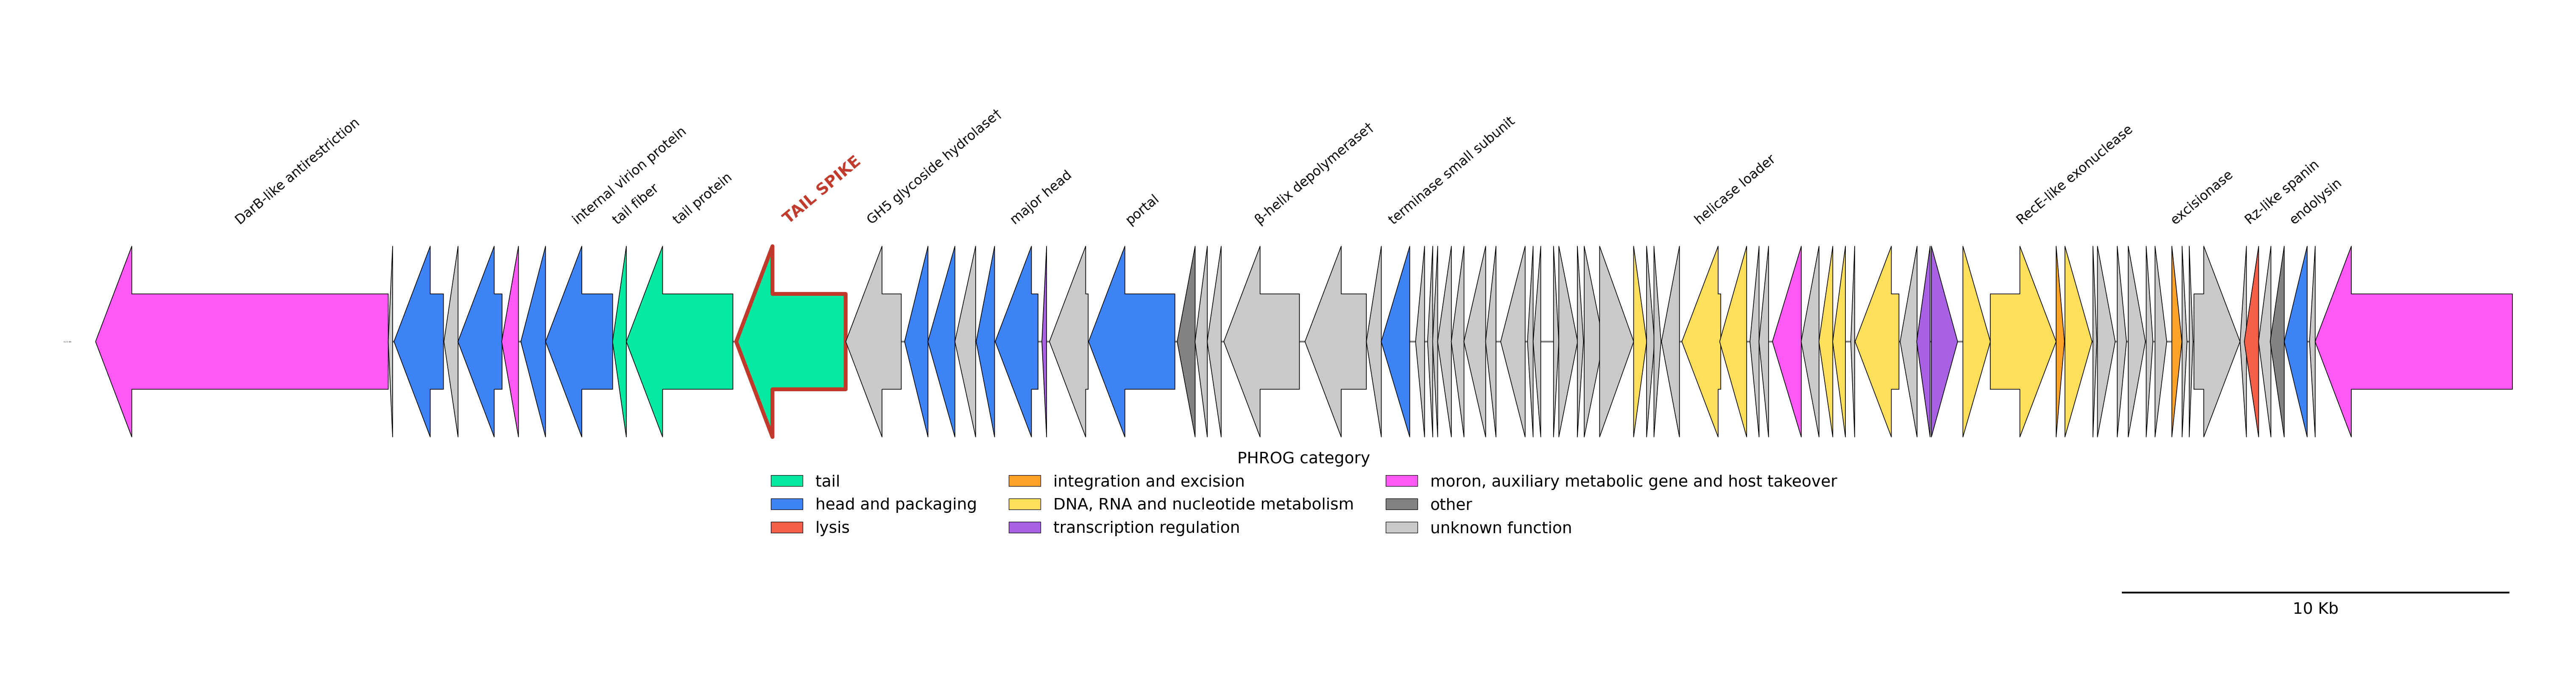
\includegraphics[width=0.95\textwidth]{fig/phage_map_banner.png}
  \end{center}
  \vspace{2pt}
  \begin{center}
  {\scriptsize\color{muted} Phage 9-2-1 $\Phi$8 — 62 kb, 80 genes — and three self-isolated
   \textit{Pseudomonas} strains\par
   \vspace{3pt}
   Chun-Yu (Alex) Chen \quad|\quad Phagenomics, Claremont CA \quad|\quad
   PI: J. Cesar Ignacio-Espinoza \quad|\quad 2026-08-21}
  \end{center}
  \note{
  Good evening. We are trying to build phage parts on purpose — to take the protein that decides which
  bacterium a phage can infect, and redesign it. Tonight: the two things you need before you can.\par
  ($\approx$18 s)}
\end{frame}

% ---------------------------------------------------------------- 2. context / goal
\begin{frame}[shrink=5]{We want to design the part, not just describe the phage}
  \begin{columns}[T,onlytextwidth]
    \begin{column}{0.53\textwidth}
      \footnotesize
      \begin{itemize}\setlength\itemsep{5pt}
        \item Phages hunt bacteria, and one phage usually infects \textbf{one strain} and ignores the
              next one over. Matching is done by \textbf{trial and error} today.
        \item Why now: \textcolor{cwzz}{\textbf{[AMR figure + source — Alex]}}. A phage is only useful
              if it hits the strain that is actually making someone sick.
        \item Our goal is a \textbf{part you can re-aim}: rebuild the receptor-binding protein so the
              same phage attacks a different strain.
        \item \textbf{We work on our own material} — local soil and water $\rightarrow$
              \textit{Pseudomonas} hosts and their phages, sequenced in house.
      \end{itemize}
      \vspace{4pt}
      \colorbox{accent!10}{\parbox{0.95\textwidth}{\centering\footnotesize
      \textbf{Tonight:} 5 isolates $\rightarrow$ \textbf{3 strains}, and one complete phage genome}}
    \end{column}
    \begin{column}{0.45\textwidth}
      \centering
      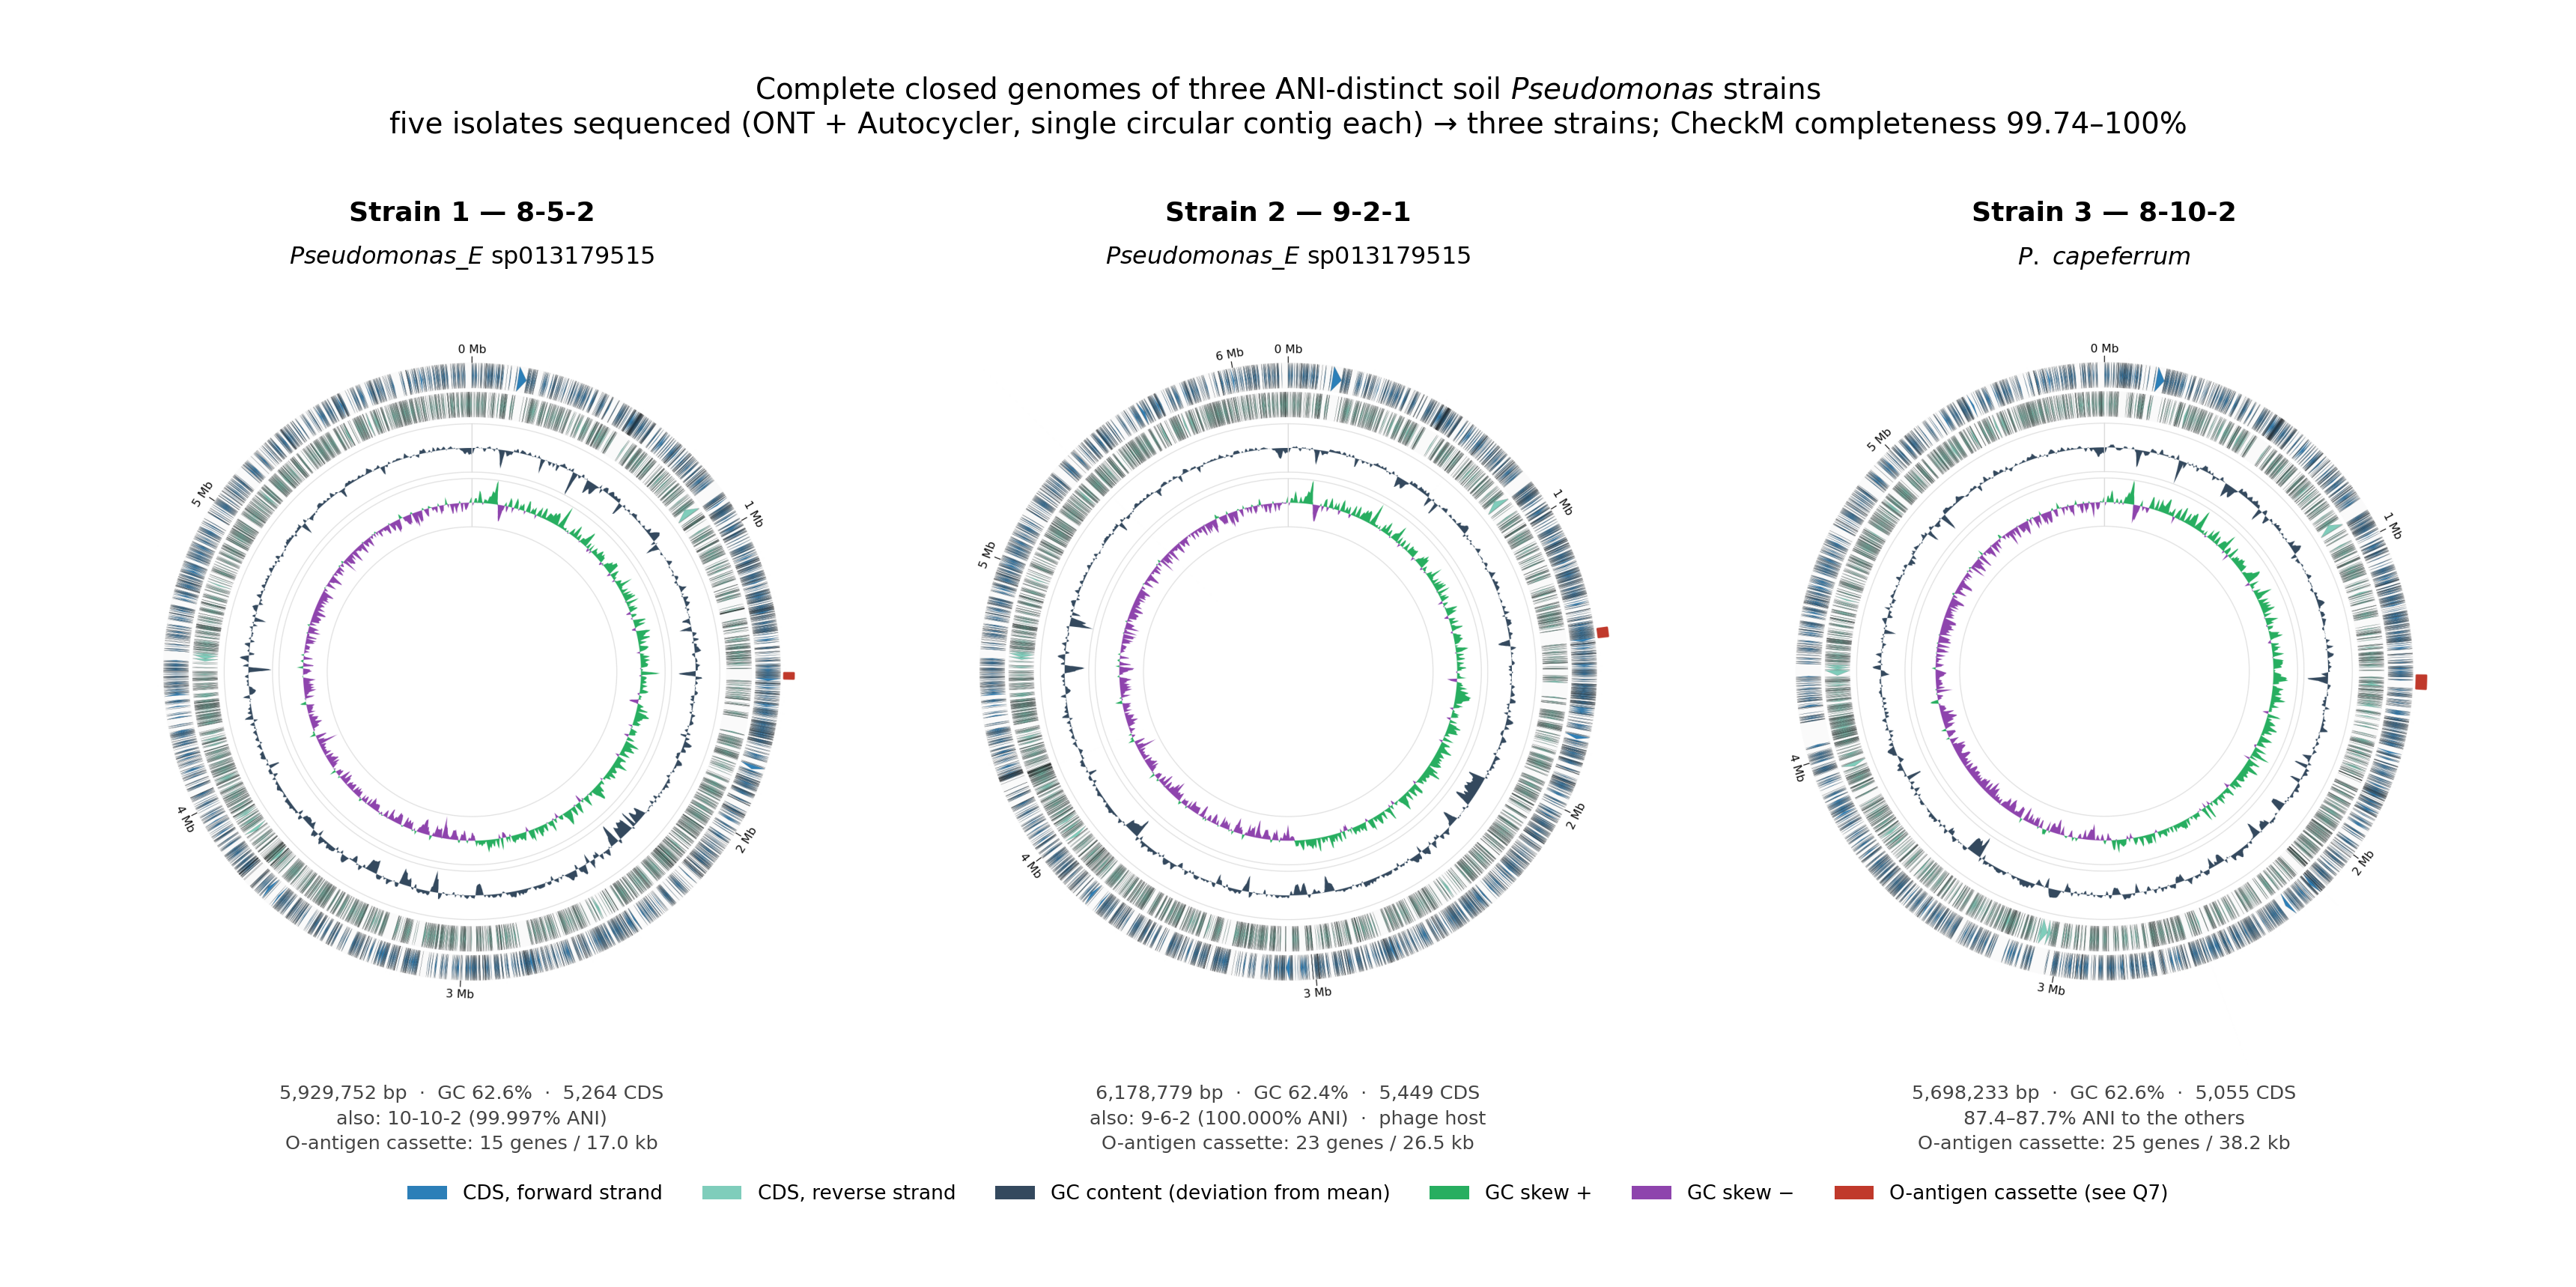
\includegraphics[width=0.98\textwidth]{../../code/output/0729_prof_figures/fig_bacterial_genomes.png}\\
      {\scriptsize\color{muted} three closed host genomes, 5.7–6.2 Mb}\\[5pt]
      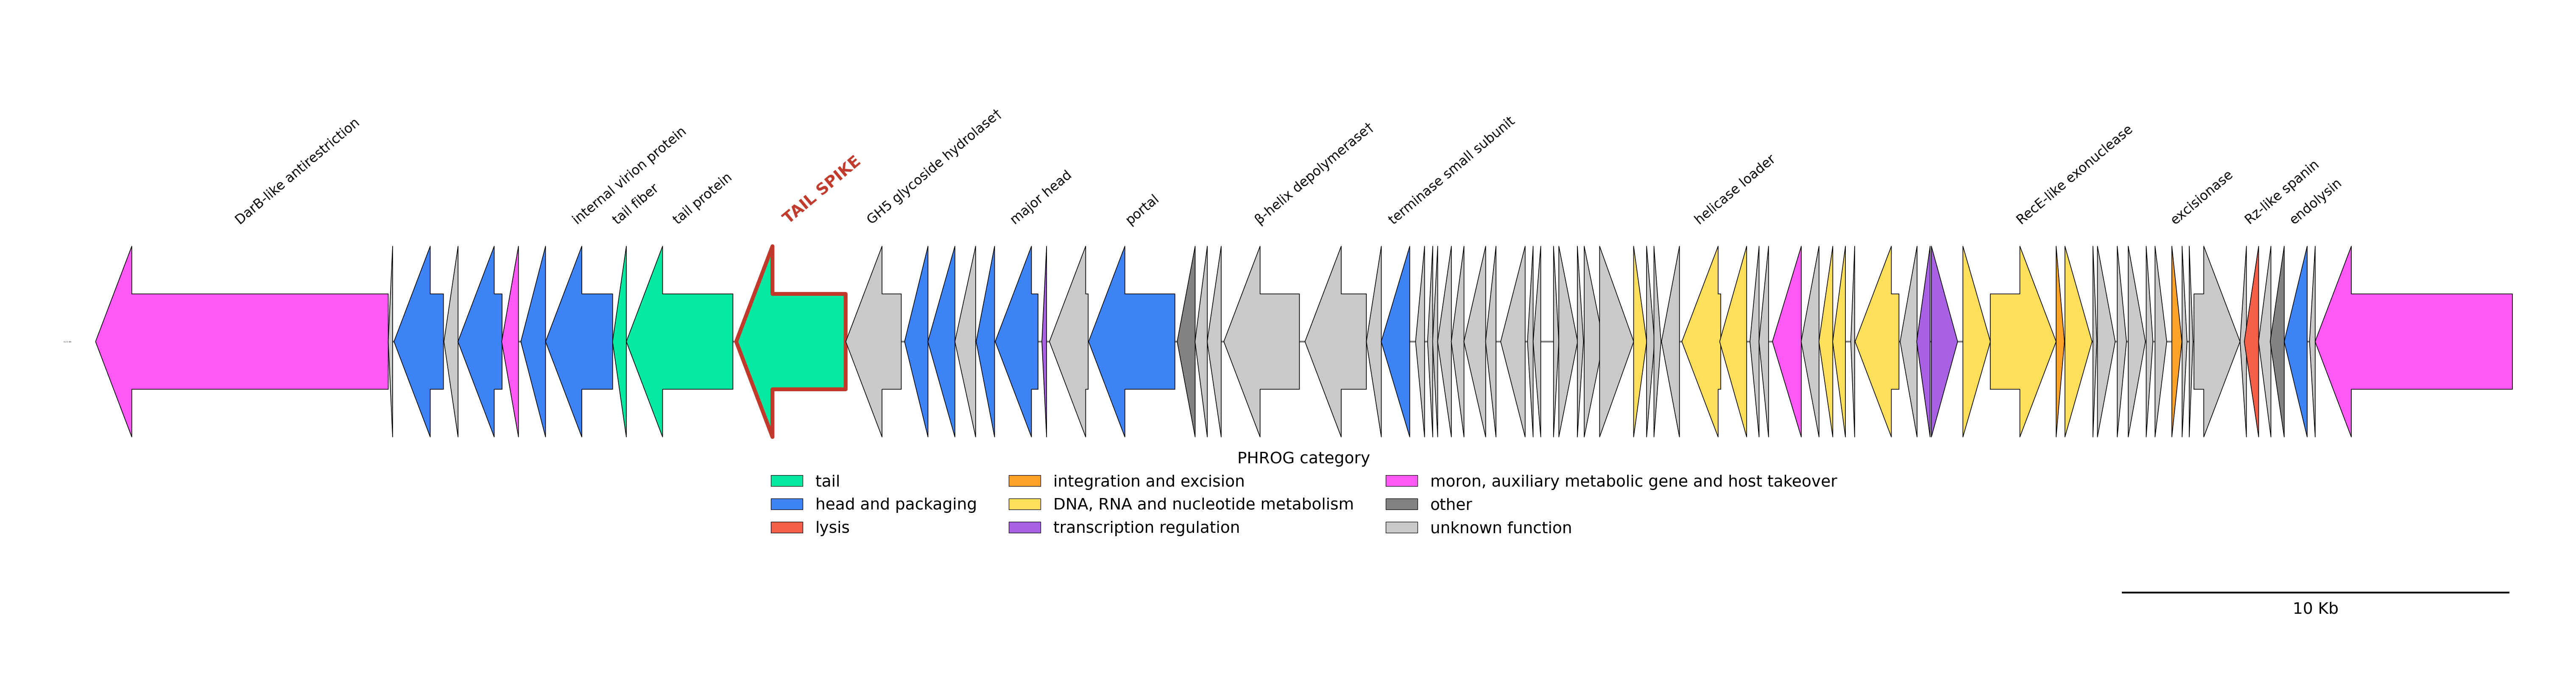
\includegraphics[width=0.98\textwidth]{fig/phage_map_banner.png}\\
      {\scriptsize\color{muted} the phage: 62 kb, 80 CDS, linear + 77 bp DTR}
    \end{column}
  \end{columns}
  \note{
  Phages hunt bacteria, and they are picky: one phage infects one strain and ignores the next one
  over. Today that match is trial and error.\par
  That matters right now — [AMR number, Alex fills in]. A phage is only useful if it hits the strain
  making someone sick.\par
  So our goal is not to describe a phage; it is to build a part you can re-aim — rebuild the
  receptor-binding protein so the same phage attacks a different strain.\par
  We work on our own material: local soil and water, Pseudomonas hosts and their phages, sequenced in
  house — five isolates, three strains, one complete phage genome.\par
  ($\approx$48 s)}
\end{frame}

% ---------------------------------------------------------------- 3. the design pipeline
\begin{frame}{The design loop — and where we actually are}
  \vspace{-2pt}
  \rqbox{Before you can redesign the targeting part: \textbf{which gene is it}, and \textbf{what must it recognise}?}
  \vspace{-2pt}
  \begin{center}
  \begin{tikzpicture}[
    font=\scriptsize,
    done/.style={draw=accent,line width=1.0pt,rounded corners=2pt,fill=accent!8,
                 text width=2.35cm,align=center,minimum height=1.8cm,inner sep=3pt},
    plan/.style={draw=muted,line width=0.9pt,dashed,rounded corners=2pt,fill=white,
                 text width=2.35cm,align=center,minimum height=1.8cm,inner sep=3pt},
    ar/.style={-{Stealth[length=4pt]},draw=muted,line width=0.7pt}]
    \node[done] (a) {\textbf{1. pick the gene}\\80 CDS $\rightarrow$ tail\\module: CDS\_0011,\\0012, 0024};
    \node[done,right=0.30cm of a] (b) {\textbf{2. define the\\target}\\fold it: what does\\it bind?};
    \node[plan,right=0.30cm of b] (c) {\textbf{3. learn from\\evolution}\\GH5 tree $\rightarrow$\\ancestral enzymes};
    \node[plan,right=0.30cm of c] (d) {\textbf{4. build\\variants}\\3 at Twist\\+ ancestral GH5};
    \node[plan,right=0.30cm of d] (e) {\textbf{5. test}\\fiber + depolymerase\\\emph{in trans}, 3 strains};
    \draw[ar] (a)--(b); \draw[ar] (b)--(c); \draw[ar] (c)--(d); \draw[ar] (d)--(e);
    \draw[ar,draw=muted,dashed] (e.south) -- ++(0,-0.35) -| node[pos=0.25,below,font=\scriptsize\color{muted}]{design rules} (c.south);
  \end{tikzpicture}
  \end{center}
  \vspace{2pt}
  {\scriptsize\color{muted} \tikz[baseline=-0.5ex]\draw[accent,line width=1pt,fill=accent!8] (0,0) rectangle (1.6ex,1.6ex);
   solid = has data \quad
   \tikz[baseline=-0.5ex]\draw[muted,dashed,line width=0.9pt] (0,0) rectangle (1.6ex,1.6ex);
   dashed = in progress / proposed \quad|\quad the next two slides are steps 1 and 2}
  \note{
  Here is the loop. Step one, pick the gene: of 80 genes the structural module narrows it to a
  handful — the tail spike, the GH5 beside it, and a depolymerase the annotator missed.\par
  Step two, define the target — you cannot redesign a binder without knowing what it binds.\par
  Step three is where evolution comes in. The tail spike decides who is recognised; the depolymerase
  decides what can be cut open. So we build a tree over all GH5 sequences and reconstruct ancestral
  enzymes — proteins from different points in evolution, not random mutants. Stated caveat: this
  assumes affinity tracks infection.\par
  Step four, build them: three constructs are at Twist, ancestral enzymes next. Step five, combine
  fiber and depolymerase in trans on our three strains, and feed that back as design rules.\par
  Solid boxes have data; dashed ones do not. The next two slides are steps one and two.\par
  ($\approx$62 s)}
\end{frame}

% ---------------------------------------------------------------- 4. result 1 — the part
\begin{frame}[shrink=5]{Steps 1--2: a $\beta$-helix depolymerase — the target is a sugar}
  \begin{columns}[T,onlytextwidth]
    \begin{column}{0.30\textwidth}
      \centering
      \includegraphics[height=0.60\textheight]{../../code/output/0729_prof_figures/panels/cds0011_trimer_domains.png}\\[2pt]
      {\scriptsize\color{muted} CDS\_0011 trimer, 941 aa $\times$ 3\par
       grey shaft \textbullet\ blue anchor\par
       \textcolor{accent}{\textbf{teal body}} \textbullet\ red foldon}
    \end{column}
    \begin{column}{0.68\textwidth}
      \footnotesize
      \begin{itemize}\setlength\itemsep{5pt}
        \item Right-handed \textbf{$\beta$-helix}, one rung every \textbf{15–18 residues} — the
              signature of a polysaccharide depolymerase. \textbf{This part cuts sugar}, so its target
              is the surface sugar, not a protein.
        \item The domain map is what makes it \textbf{engineerable}: pLDDT 88–94, and the body
              (res 301–941) is rigid to \textbf{0.44–0.99 \AA} across five models — that boundary is
              exactly where our construct starts (res 305).
        \item The protein--protein hypothesis was tested first \textbf{and failed}:
      \end{itemize}
      \vspace{1pt}
      \begin{center}
        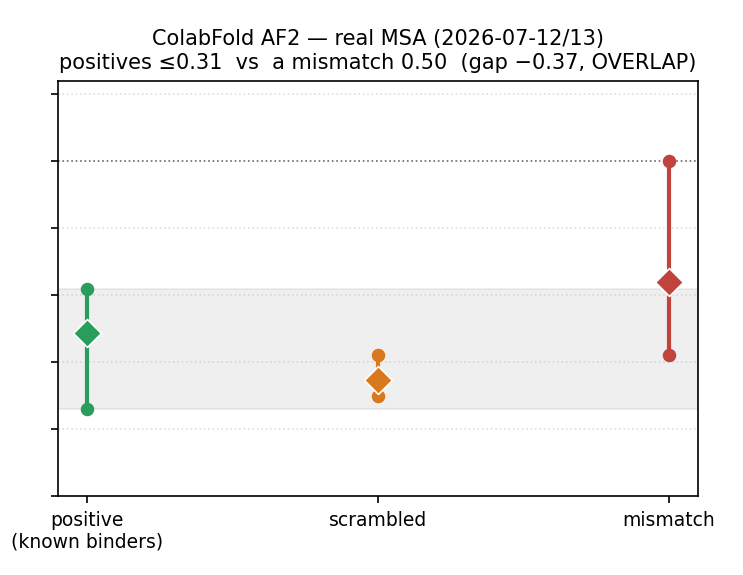
\includegraphics[height=0.25\textheight]{fig/binding_controls_af2.png}\\
        {\scriptsize\color{muted} positives ipTM $\leq$ 0.31 vs a mismatched pair 0.50 — no signal}
      \end{center}
    \end{column}
  \end{columns}
  \note{
  Steps one and two on one slide. This is the tail spike, 941 residues, a trimer: grey shaft AlphaFold
  cannot place, blue anchor into the capsid, teal working body.\par
  That body is a right-handed beta helix, one rung every 15 to 18 residues — the signature of a
  depolymerase. So the part cuts sugar, and its target is the surface sugar, not a protein.\par
  It is also engineerable: the body from residue 301 is rigid, under one angstrom across five models,
  and that boundary is exactly where our construct starts.\par
  And we tested the protein-protein hypothesis first — docking gave positives at 0.31 and a mismatch
  at 0.50. No discriminating power, so we retired that screen.\par
  ($\approx$57 s)}
\end{frame}

% ---------------------------------------------------------------- 5. result 2 — the target varies
\begin{frame}[shrink=5]{The target is different in every strain — that is the handle}
  \vspace{1pt}
  \footnotesize Same \texttt{ihfB}-flanked slot, different cargo
   \ \textcolor{muted}{(grey ribbons = homology)}\normalsize
  \vspace{1pt}
  \begin{center}
    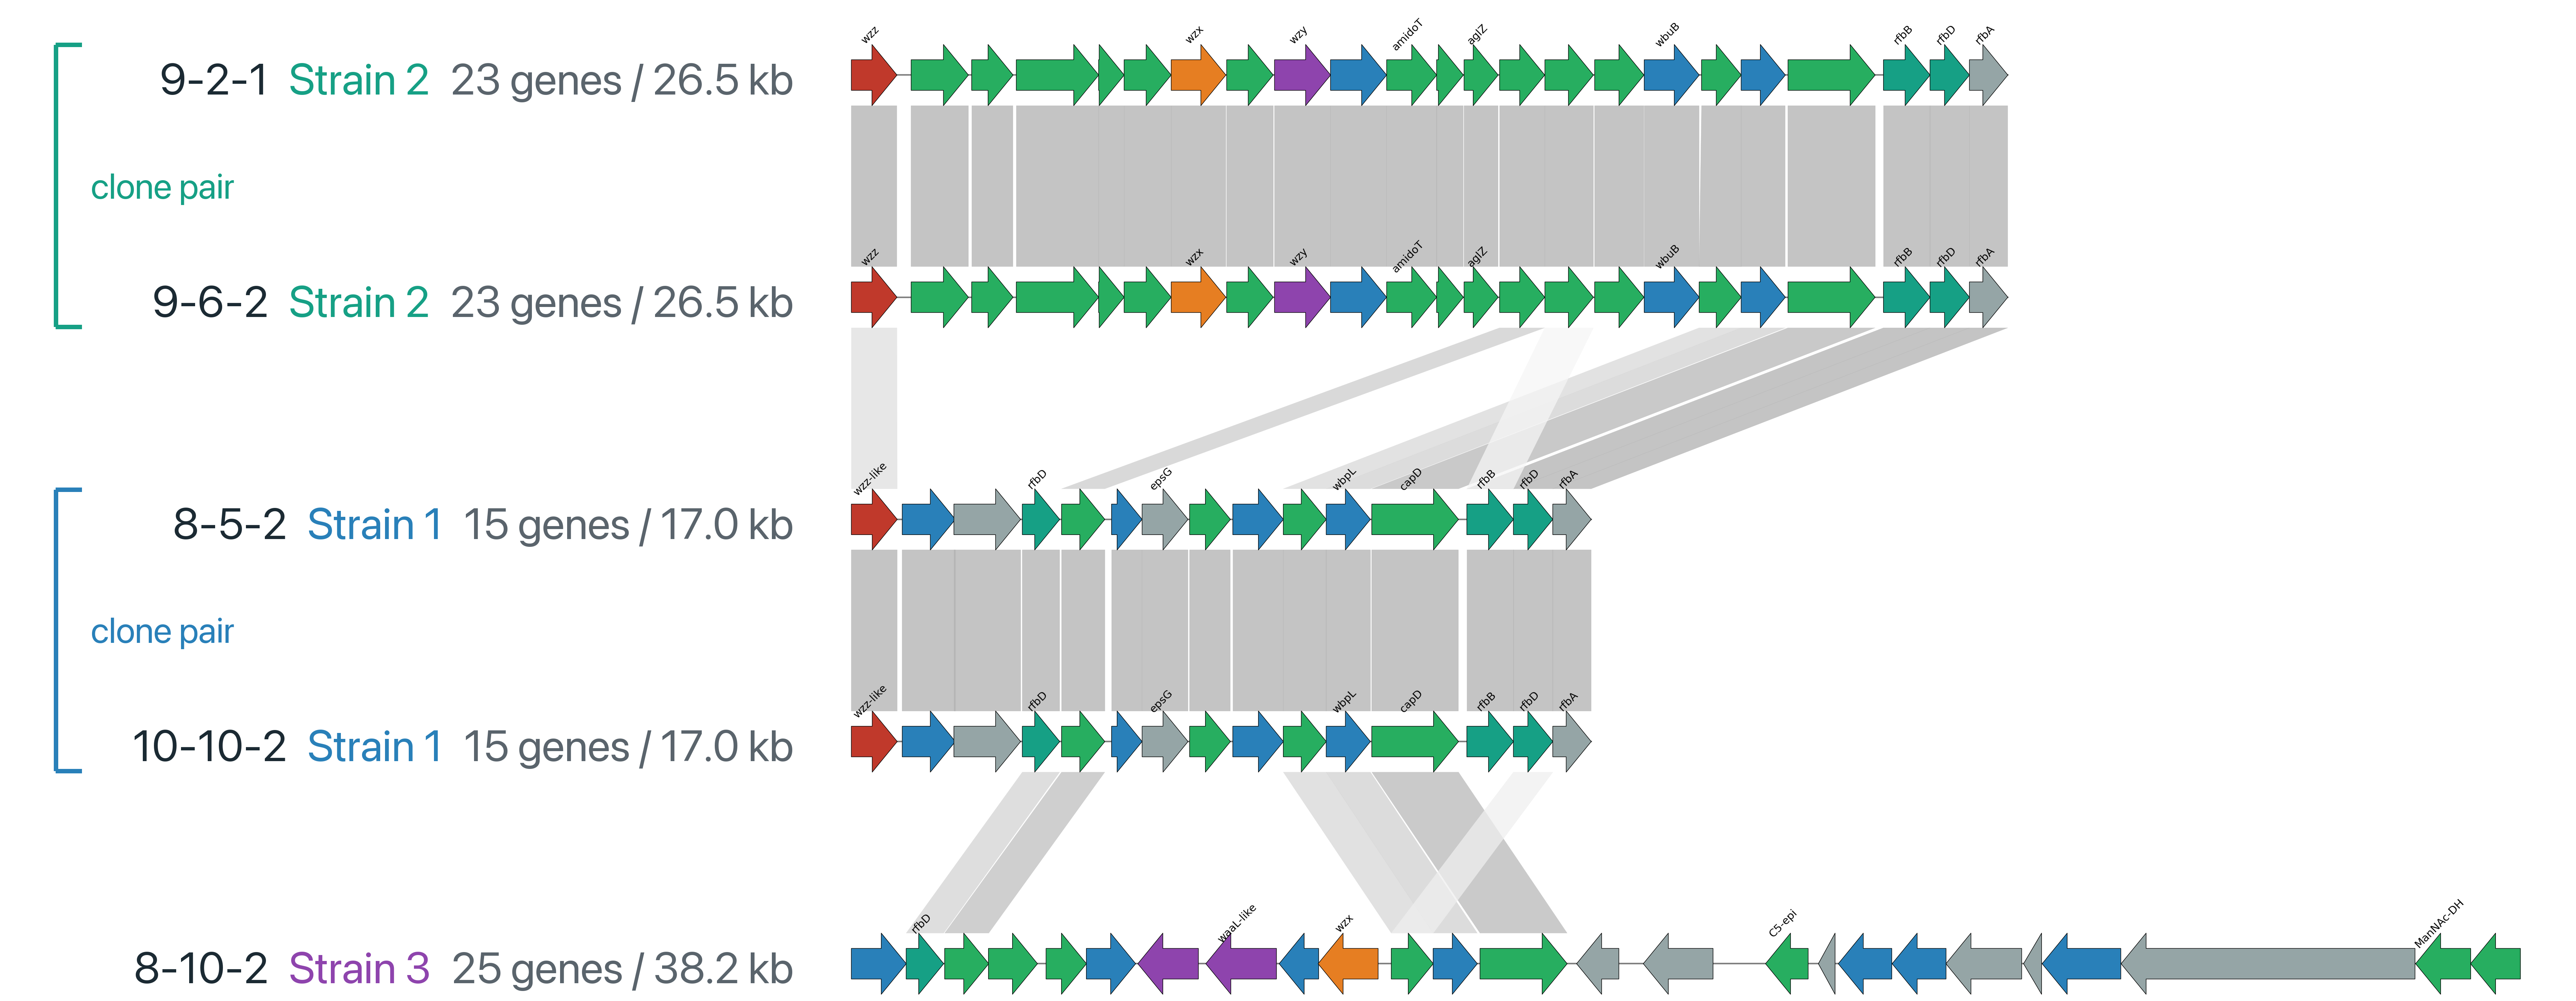
\includegraphics[width=0.95\textwidth,height=0.54\textheight,keepaspectratio]{fig/oantigen_tracks_labeled.png}
  \end{center}
  \vspace{-4pt}
  \begin{center}\tiny
    \chip{cwzz}{chain-length regulator}\quad\chip{cwzx}{flippase (wzx)}\quad\chip{cwzy}{polymerase (wzy)}\quad
    \chip{cgt}{glycosyltransferase}\quad\chip{crha}{dTDP-rhamnose}\quad\chip{cnuc}{nucleotide-sugar}\quad
    \chip{cother}{unassigned}
  \end{center}
  \vspace{1pt}
  {\footnotesize \textbf{4 of 45 clusters shared by all three} — generic sugar chemistry only, no
   shared assembly machinery. \textcolor{muted}{Control: clone pairs 100.0\% identical.}}
  \note{
  If the part reads a sugar, does that sugar differ between strains? That difference is the handle a
  redesigned part would turn.\par
  Five tracks: two Strain 2 clones, two Strain 1 clones, Strain 3; arrows are genes, grey ribbons are
  homology. Control first: inside each clone pair all 23 and all 15 genes are identical. ANI
  saturates, so this had to be measured.\par
  Across strains the links are sparse and crossed — of 45 clusters only four are shared, all generic
  sugar chemistry, no shared flippase, polymerase or chain-length regulator.\par
  Three strains, three targets. This phage should not plaque on the other two, and a re-aimed part is
  what would change that.\par
  ($\approx$57 s)}
\end{frame}

% ---------------------------------------------------------------- 6. close
\begin{frame}[shrink=5]{Where the loop stands}
  \begin{columns}[T,onlytextwidth]
    \begin{column}{0.50\textwidth}
      \small
      \textcolor{accent}{\textbf{Conclusion}}\\
      We know \textbf{which gene} to engineer and \textbf{what it must recognise}: the tail-spike
      depolymerase, against a strain-specific O-antigen — and our three strains give three different
      targets.
      \vspace{6pt}

      \textcolor{accent}{\textbf{Limitation}}\\
      Steps 3–5 are \textbf{not results yet}: the GH5 ancestral reconstruction is still being built,
      the constructs are not expressed, and the cross-strain plaque assay was run July 4 but the data
      is not in our hands. It also assumes affinity tracks infection. No serotyping tool exists for
      this taxon, so we cannot name an O-type.
      \vspace{6pt}

      \textcolor{accent}{\textbf{Next three months}}\\
      Recover that readout; express the three constructs; reconstruct ancestral GH5 enzymes and test
      fiber $+$ depolymerase \emph{in trans} on the three strains. The tail spike also has a
      15,775-sequence alignment — enough for a conservation profile on the structure.
    \end{column}
    \begin{column}{0.48\textwidth}
      \centering
      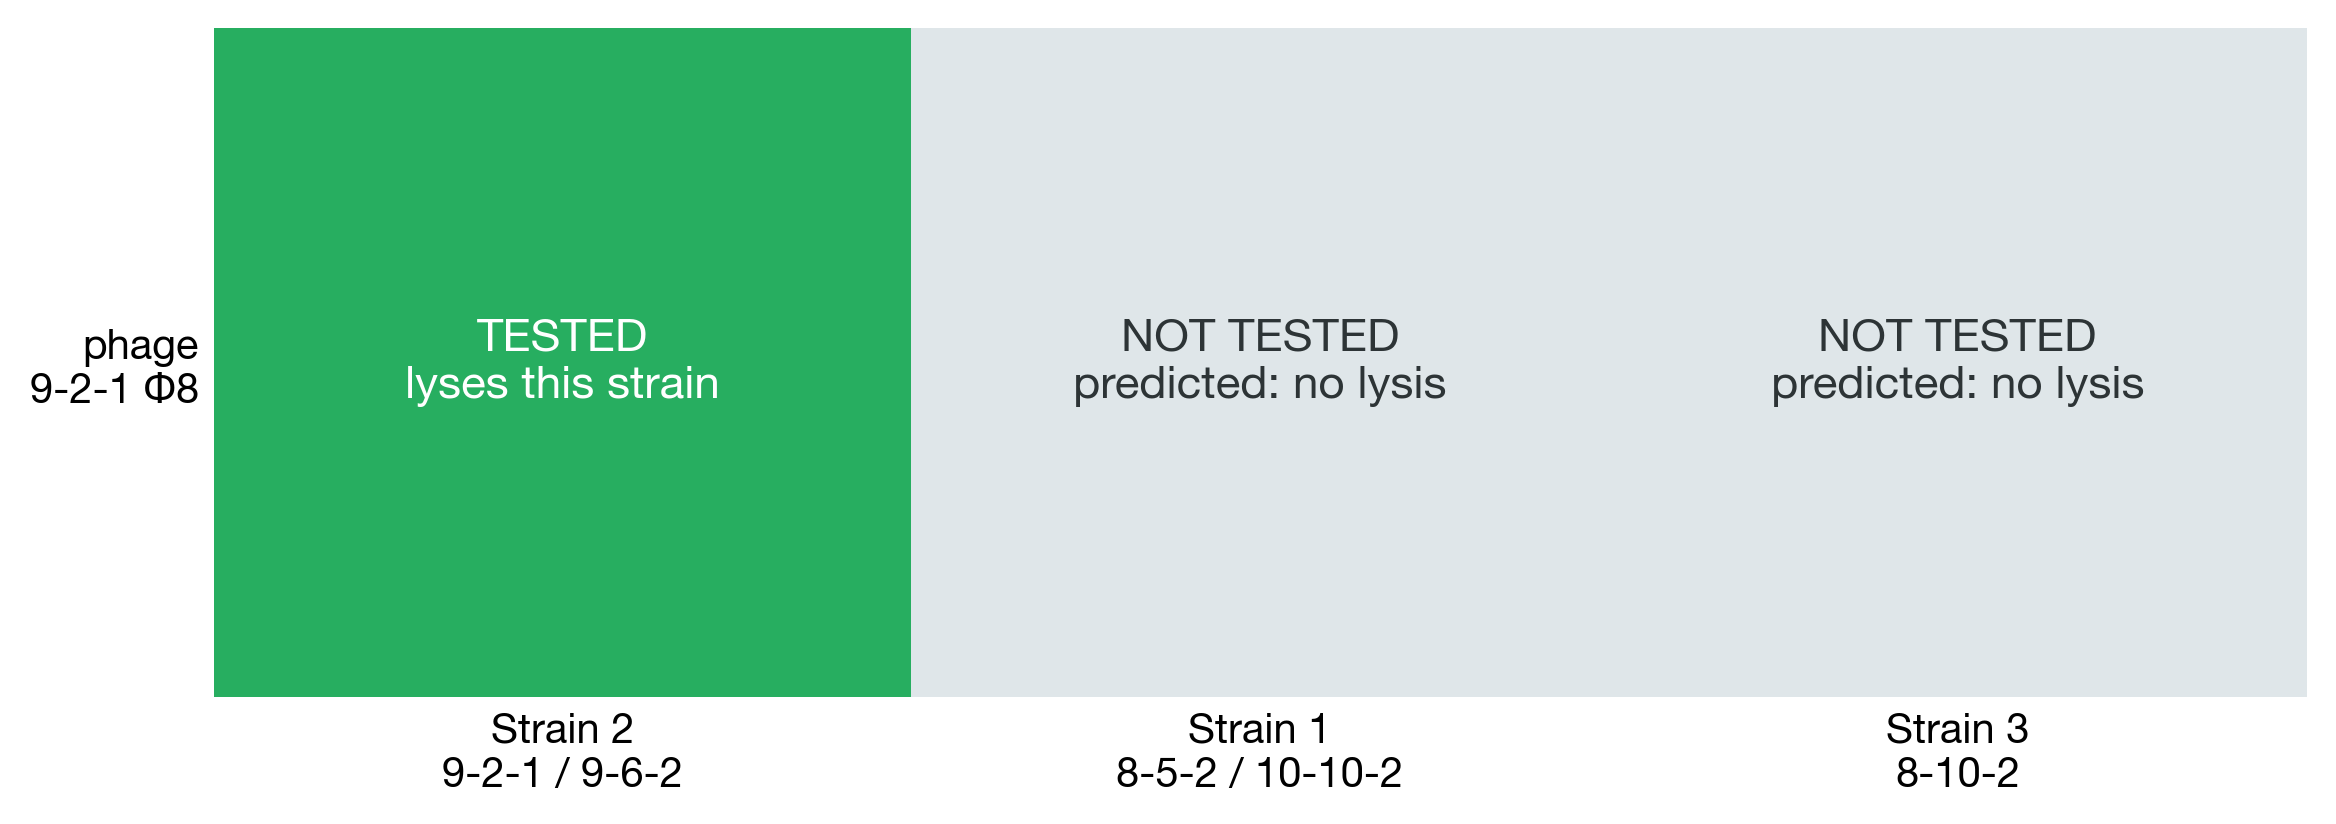
\includegraphics[width=\textwidth]{fig/hostrange_cells.png}\\[3pt]
      {\scriptsize\color{muted} only Strain 2 has actually been challenged; the grey cells are
       predictions, and the July 4 assay reads them out}\\[8pt]
      \begin{flushleft}\scriptsize
      \textcolor{accent}{\textbf{1. pick the gene}} — done\\
      \textcolor{accent}{\textbf{2. define the target}} — done\\
      \textcolor{muted}{\textbf{3. ancestral GH5 enzymes} — PI building the tree}\\
      \textcolor{muted}{\textbf{4. build} — 3 constructs at Twist}\\
      \textcolor{muted}{\textbf{5. test} — \emph{in trans}, waiting on the July 4 readout}
      \end{flushleft}
    \end{column}
  \end{columns}
  \vspace{5pt}
  \begin{center}\large\bfseries We now know which part to rebuild and what it has to grip — the
   ancestral variants are the next lever.\end{center}
  \note{
  Where the loop stands. We know which gene to engineer and what it must recognise — the tail-spike
  depolymerase against a strain-specific O-antigen — and three strains give three targets.\par
  The limitation is honest: steps three to five are not results — the GH5 tree is still being built,
  the constructs are not expressed, and the July fourth plaque data is not in our hands. And no
  serotyping tool exists for this taxon, so we cannot name an O-type.\par
  Next three months: recover that readout, express the constructs, and reconstruct ancestral GH5
  enzymes — then measure how proteins from different points in evolution behave with the fiber, in
  trans, on the three strains.\par
  We know which part to rebuild and what it has to grip. The ancestral variants are the next lever.\par
  ($\approx$58 s — stop here, not on a thank-you slide)}
\end{frame}

% ================================================================ backup
\begin{frame}[plain]
  \vspace{1.2cm}\centering{\Large\bfseries Backup}\\[4pt]{\color{muted} not shown unless asked}
\end{frame}

\begin{frame}{Backup 1 — gene selection and the constructs}
  \small
  \begin{itemize}\setlength\itemsep{5pt}
    \item Structural module, in canonical podovirus order: portal (CDS\_0020) $\rightarrow$ major
          capsid (0017) $\rightarrow$ adaptors $\rightarrow$ \textbf{tail spike (0011)} $\rightarrow$
          tail (0010) $\rightarrow$ fiber (0009).
    \item \textbf{CDS\_0024 is a second $\beta$-helix depolymerase} (rung 22–24) that Pharokka called
          ``hypothetical''; the de-novo RBP classifier found it at score 0.998.
    \item \textbf{CDS\_0012 is a GH5 glycoside hydrolase} — a separate protein, not a domain of the
          tail spike; all four AF3 templates are GH5 endoglucanases.
    \item Ordered from Twist 2026-07-27, all in pET-28a(+) with N-terminal His6:
          CDS\_0011 res \textbf{305–941} (the rigid body), CDS\_0010 res 105–917,
          CDS\_0012 res 117–477.
    \item CDS\_0010 is an \textbf{unknown protein} — the glycosidase call was withdrawn 2026-07-29;
          it is being expressed for functional characterisation.
  \end{itemize}
\end{frame}

\begin{frame}{Backup 2 — how the locus was pulled, how orthology was called}
  \small
  \begin{itemize}\setlength\itemsep{5pt}
    \item Anchor, identical in all five genomes: 30S ribosomal protein S1 $\rightarrow$ \texttt{ihfB}
          $\rightarrow$ LPS assembly protein A $\rightarrow$ MBL-fold hydrolase $\rightarrow$
          \textbf{cassette starts}. \texttt{ihfB} is the canonical upstream flank of the
          \textit{Pseudomonas} OSA cluster in the literature.
    \item Orthology = MMseqs2 clustering, $\geq$30\% identity / $\geq$50\% coverage.
          \textbf{Product names cannot be used}: the chain-length regulators of Strain 1 and Strain 2
          carry different Bakta labels but are homologous by sequence.
    \item Locus sizes: Strain 2 = 23 genes / 26.5 kb \textbullet\ Strain 1 = 15 / 17.0 kb \textbullet\
          Strain 3 = 25 / 38.2 kb.
    \item The cross-strain best-hit numbers (9/23, 10/23, 6/15) are one-directional best hits at a
          looser cutoff and are not meant to reconcile with the 45/4 cluster counts.
  \end{itemize}
\end{frame}

\begin{frame}{Backup 3 — cluster matrix, 45 clusters $\times$ 3 strains}
  \centering
  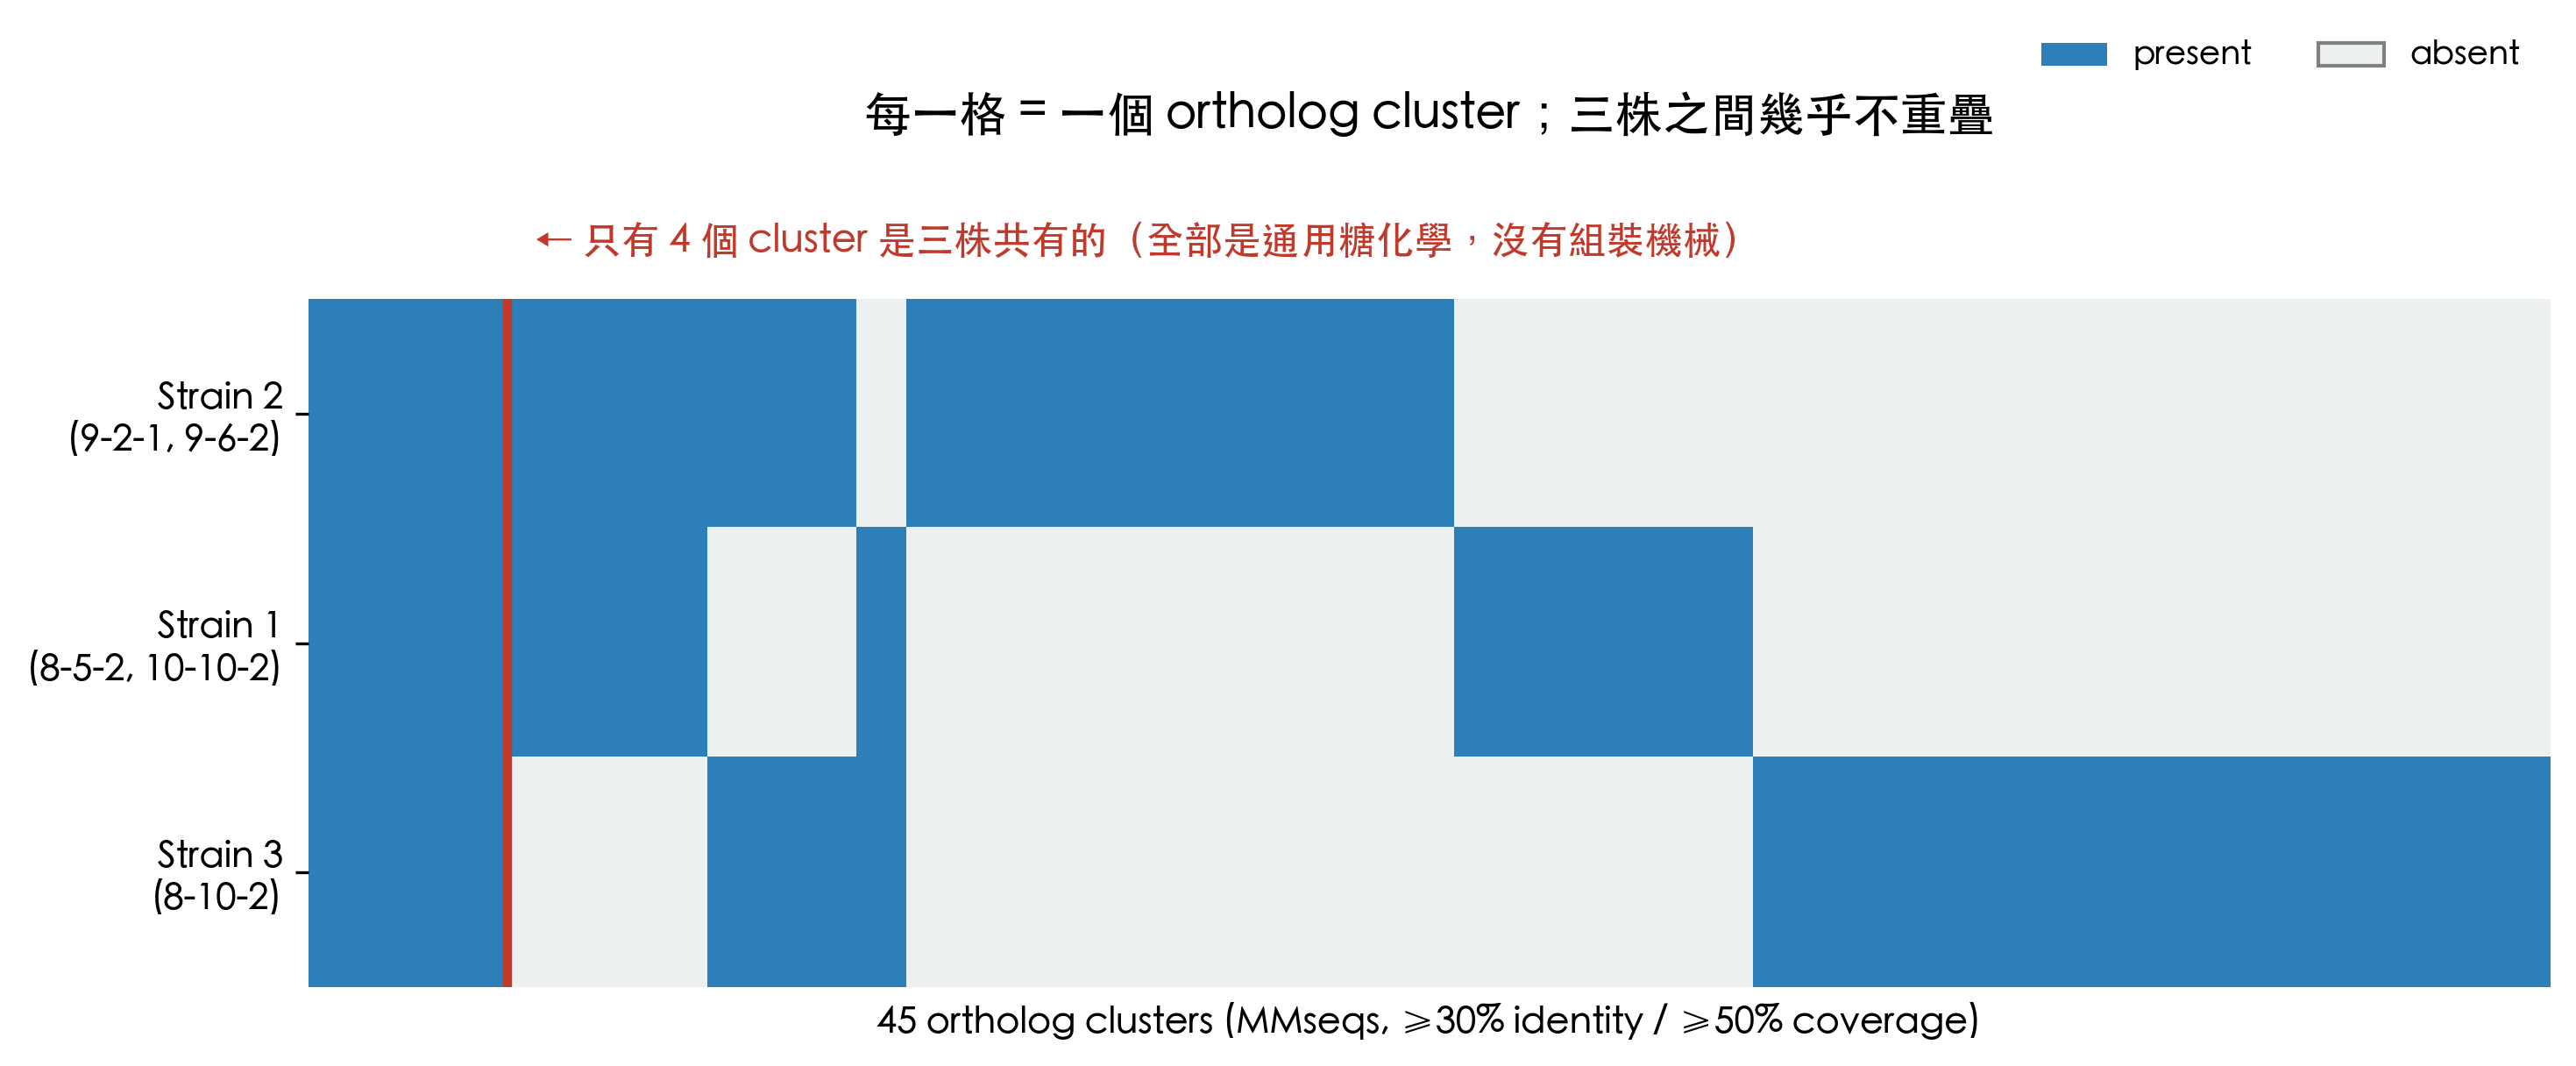
\includegraphics[width=0.86\textwidth,height=0.74\textheight,keepaspectratio]{../../code/output/0727_o_antigen_comparison/fig2_cluster_presence.png}
\end{frame}

\begin{frame}{Backup 4 — limitations in full}
  \small
  \begin{itemize}\setlength\itemsep{5pt}
    \item \textbf{Variable $\neq$ specificity-determining.} An earlier plan to read specificity off
          metagenomic variable regions was rejected in our own review: metagenome sequences carry no
          host labels, so specificity-determining positions cannot be identified that way. The
          15,775-sequence alignment (tail spike, CDS\_0011) supports a \textbf{conservation profile}
          — not ``these residues set the host range''. The ancestral reconstruction the PI is building
          is a separate thing: a tree over \textbf{all GH5 sequences} (CDS\_0012), whose ancestral
          enzymes get expressed and challenged \emph{in trans}, under the stated caveat that
          affinity $\sim$ binding $\sim$ infection.
    \item \textbf{Do not say Strain 1 lacks a flippase or polymerase} — Bakta assigns no Pfam/InterPro
          to those two genes; confirming them needs InterProScan.
    \item \textbf{The sugar structure has not been measured} — gene content is not structure; that
          needs LPS extraction and mass spectrometry.
    \item \textbf{The $\beta$-helix has no named structural homolog yet} — no foldseek or DALI run.
    \item \textbf{Taxonomy}: the virion module is podovirus-like, but reciprocal best hits against T7,
          $\varphi$KMV and KP32 are $\approx$0 and the genome carries an excisionase; \textit{terL} is
          unannotated, so formal taxonomy cannot be run. ``T7-like'' is an organizational analogy only.
  \end{itemize}
\end{frame}

\begin{frame}{Backup 5 — the three host genomes}
  \centering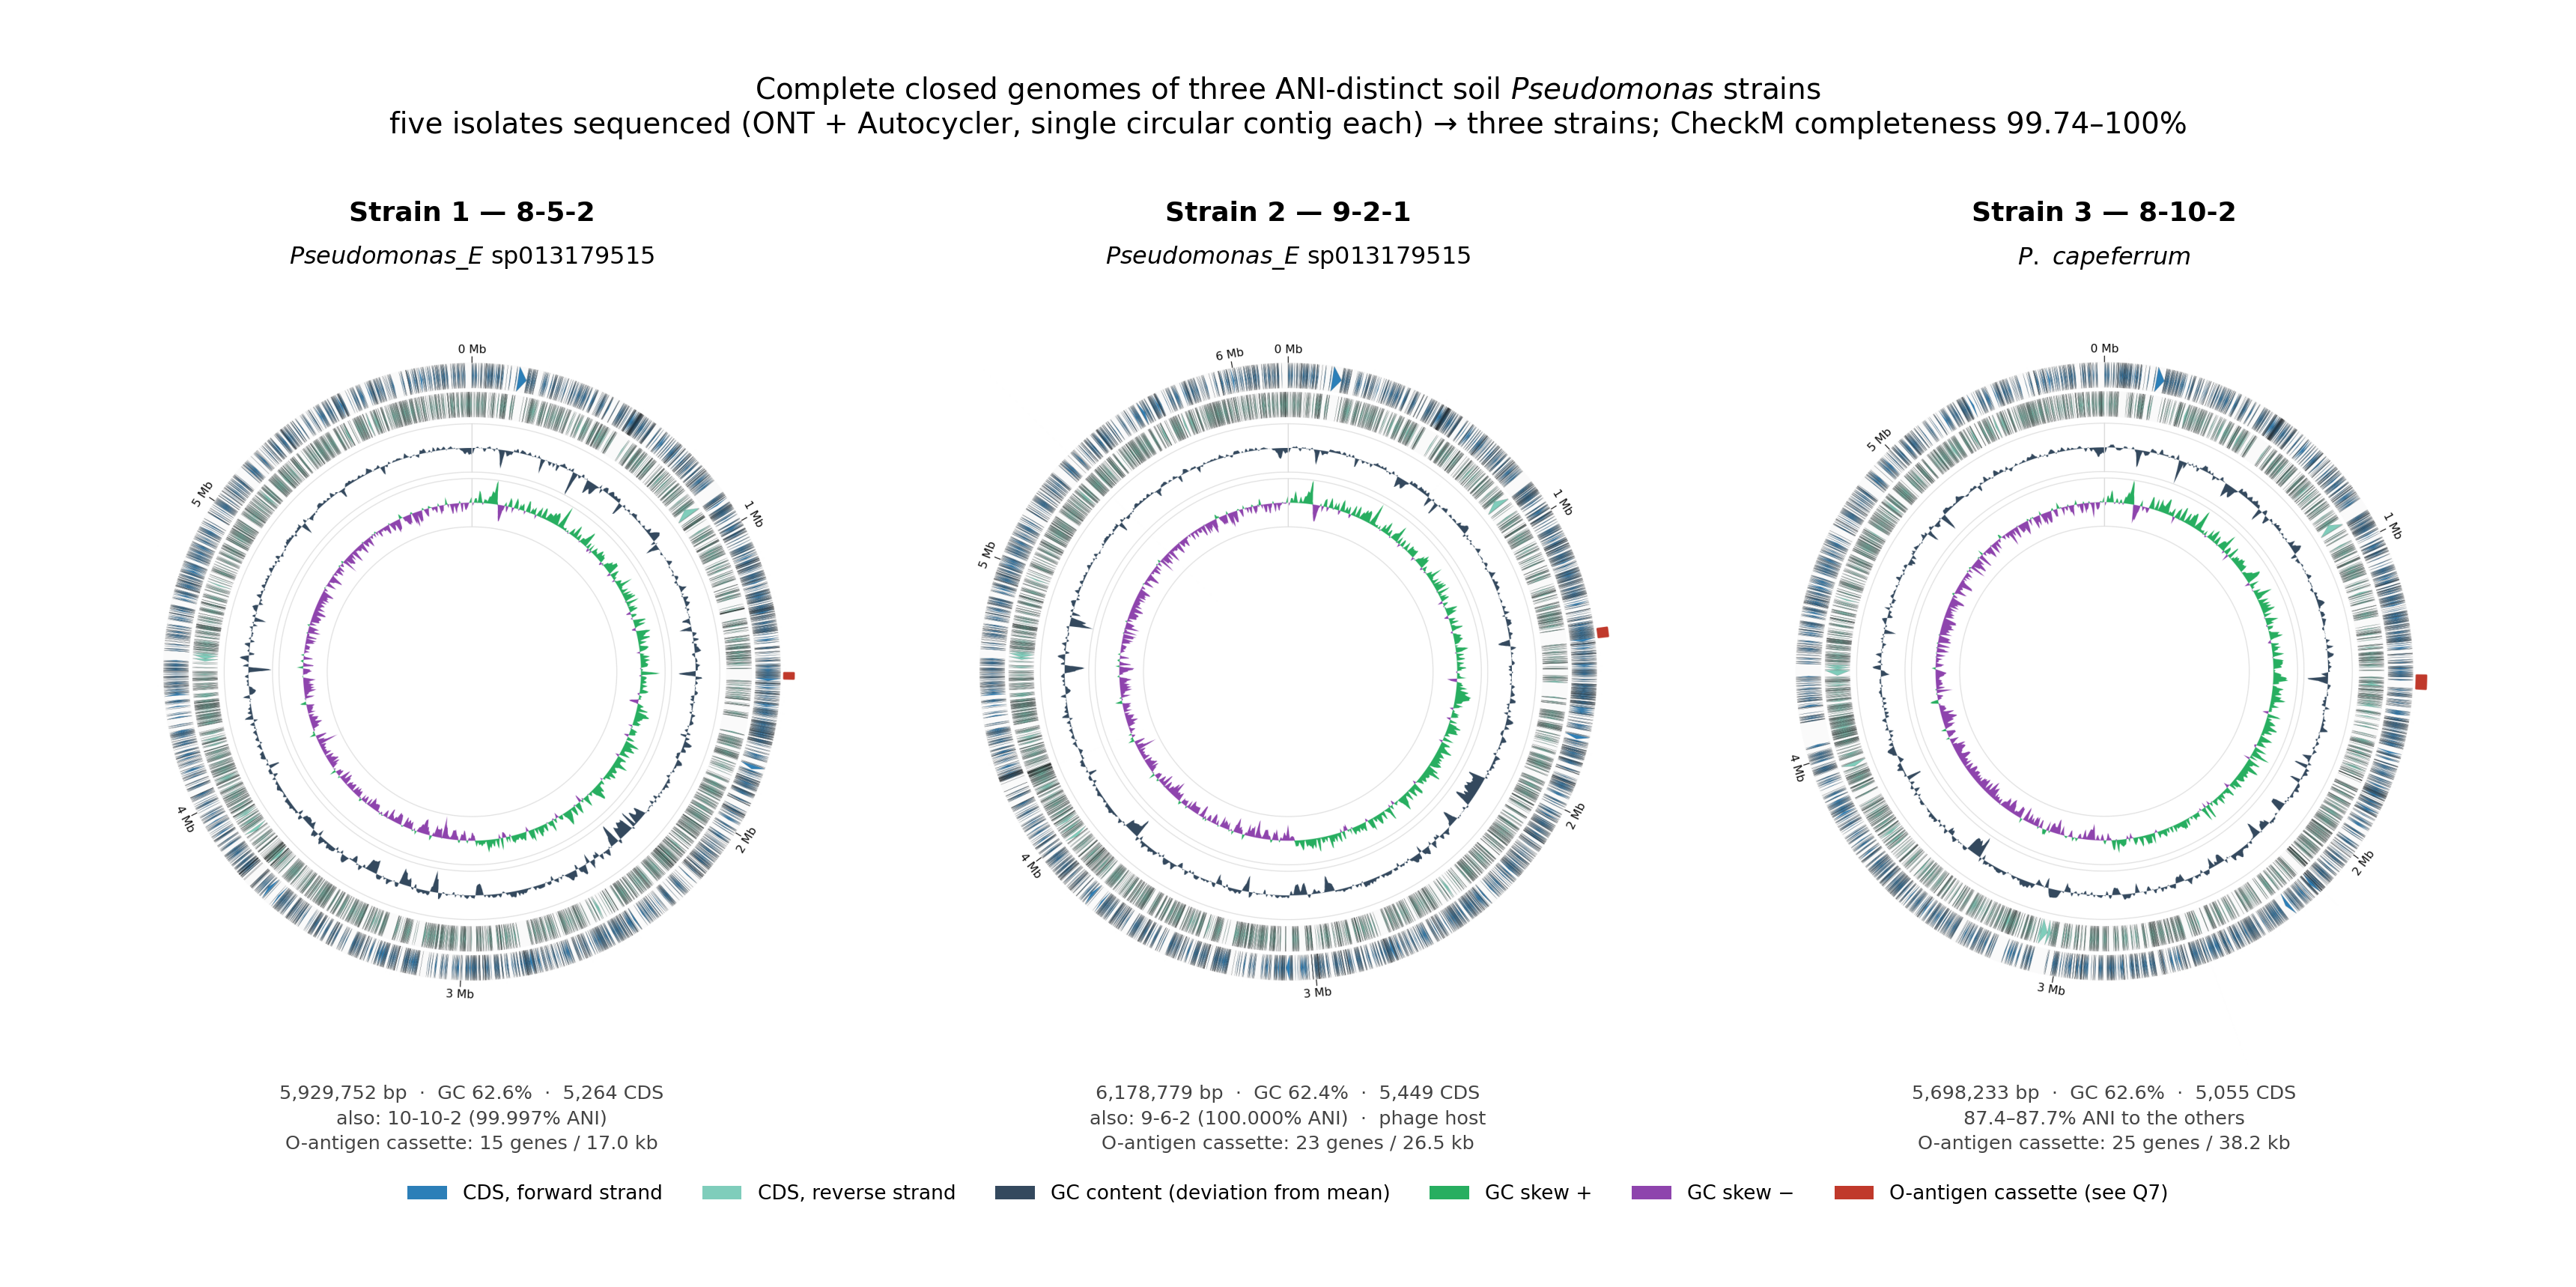
\includegraphics[width=0.95\textwidth,height=0.78\textheight,keepaspectratio]{../../code/output/0729_prof_figures/fig_bacterial_genomes.png}
\end{frame}

\begin{frame}{Backup 6 — phage genome, tail / RBP module}
  \centering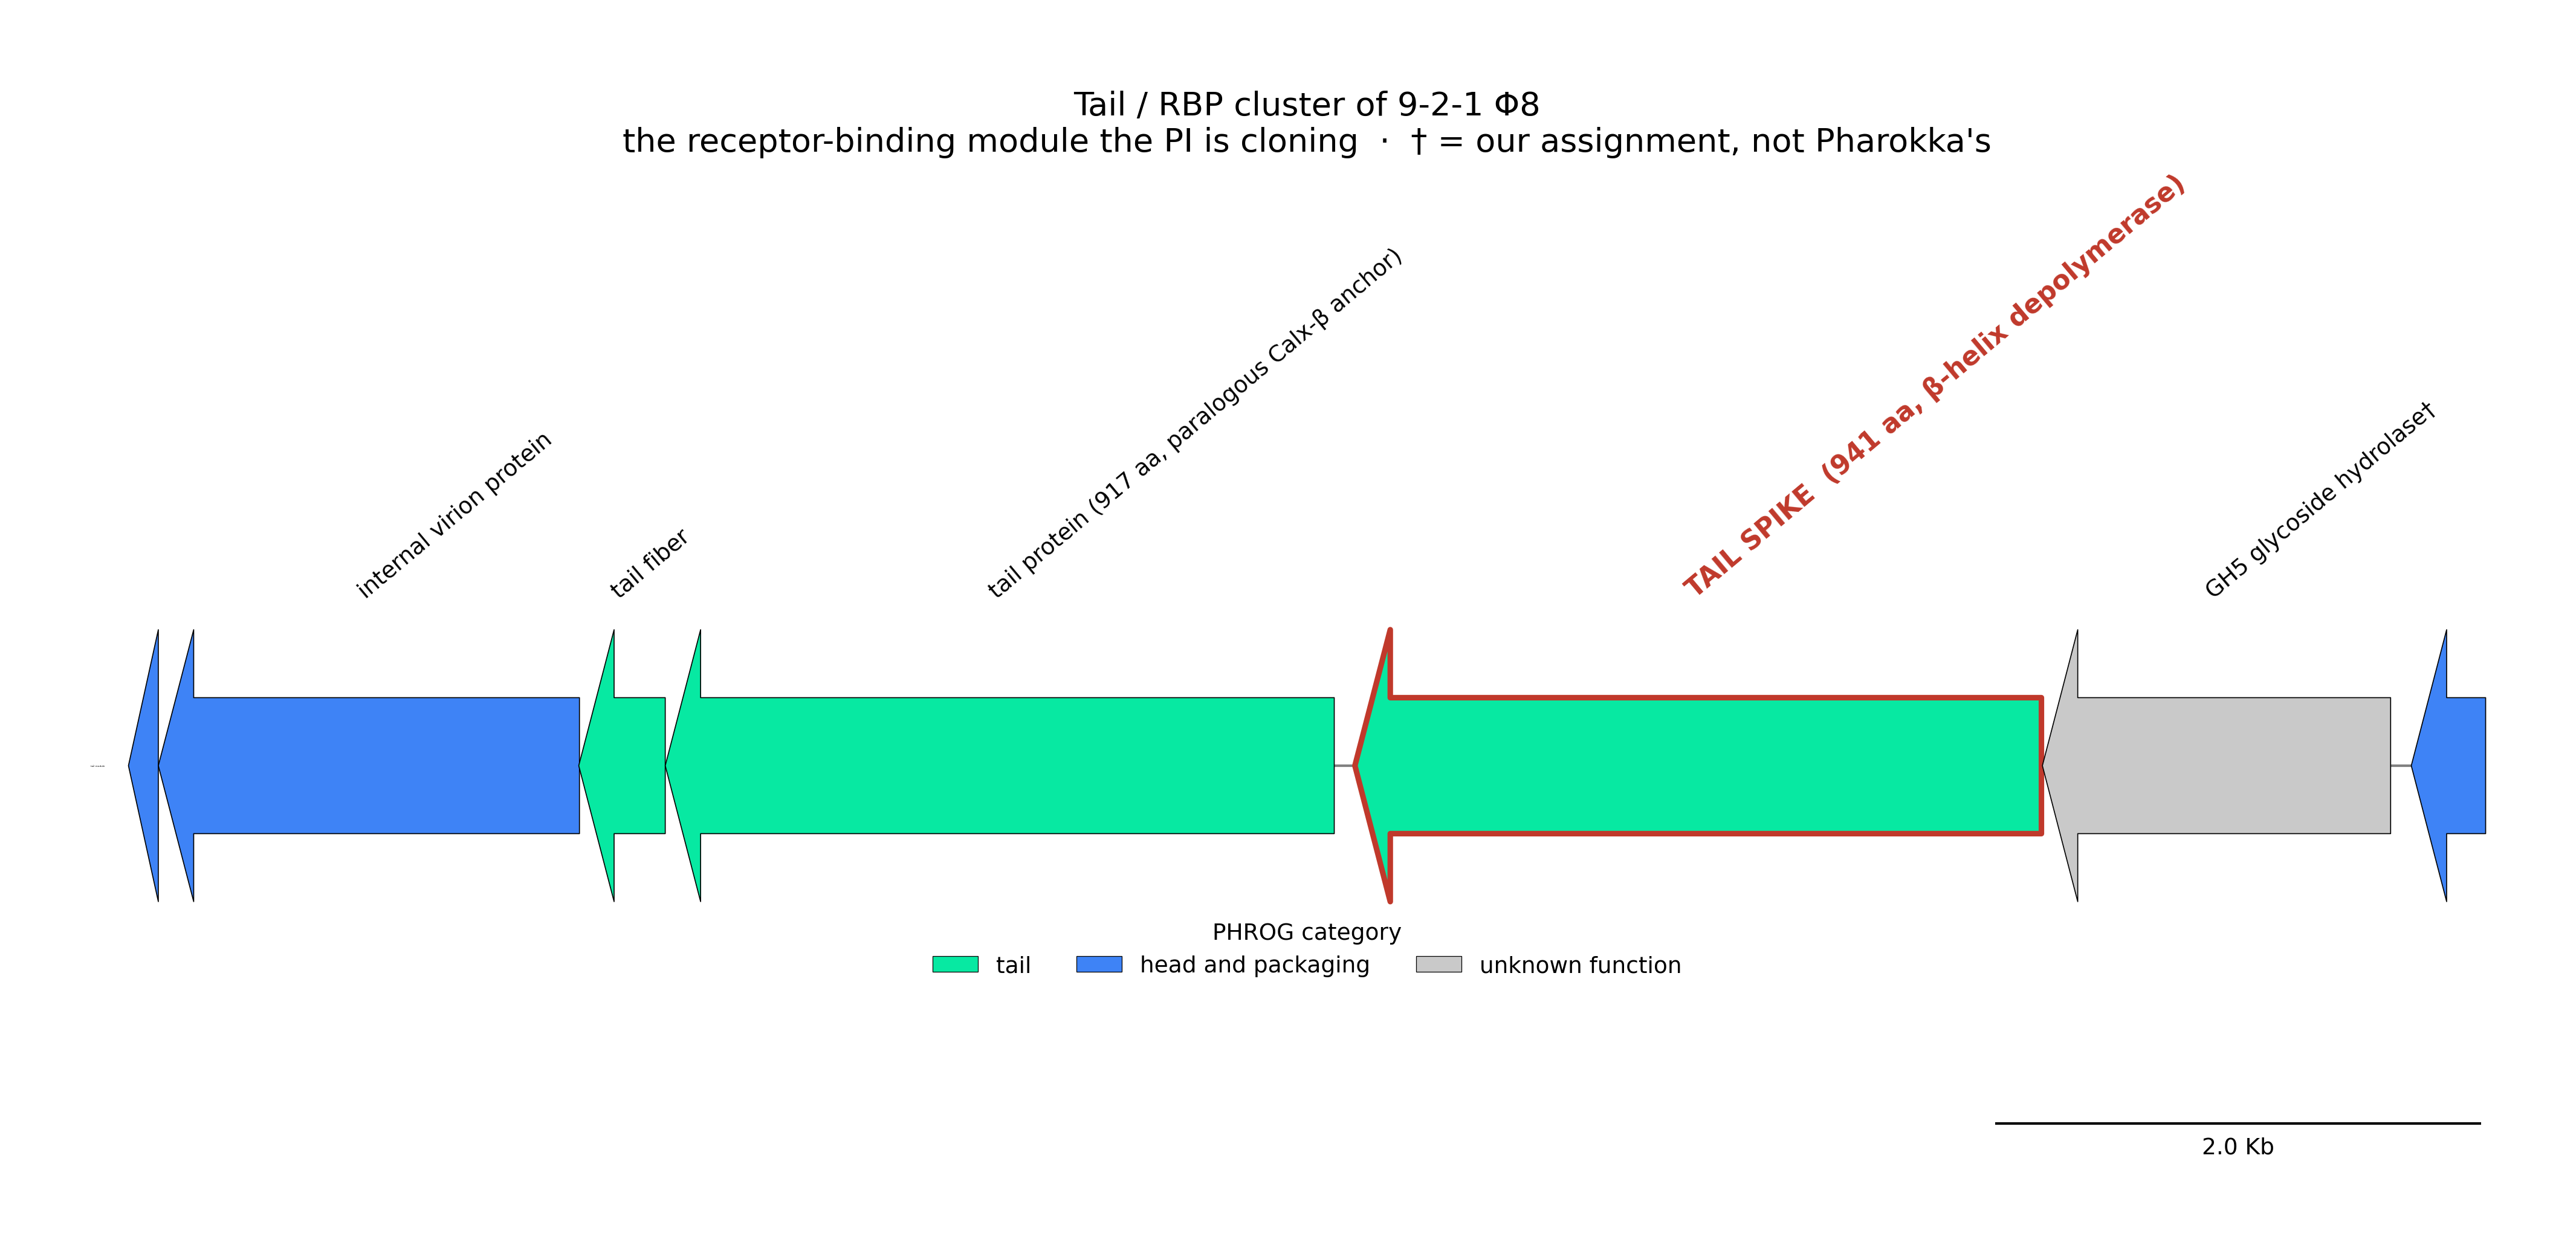
\includegraphics[width=0.98\textwidth,height=0.70\textheight,keepaspectratio]{../../code/output/0729_prof_figures/fig_phage_tail_module.png}\\
  {\scriptsize\color{muted} Numbering is the PI's \texttt{UUAIURNK\_}. The old 0708 genome map is
   mirrored — do not reuse it.}
\end{frame}

\begin{frame}{Backup 7 — enzymatic domains in full (incl.\ CDS\_0012 GH5)}
  \centering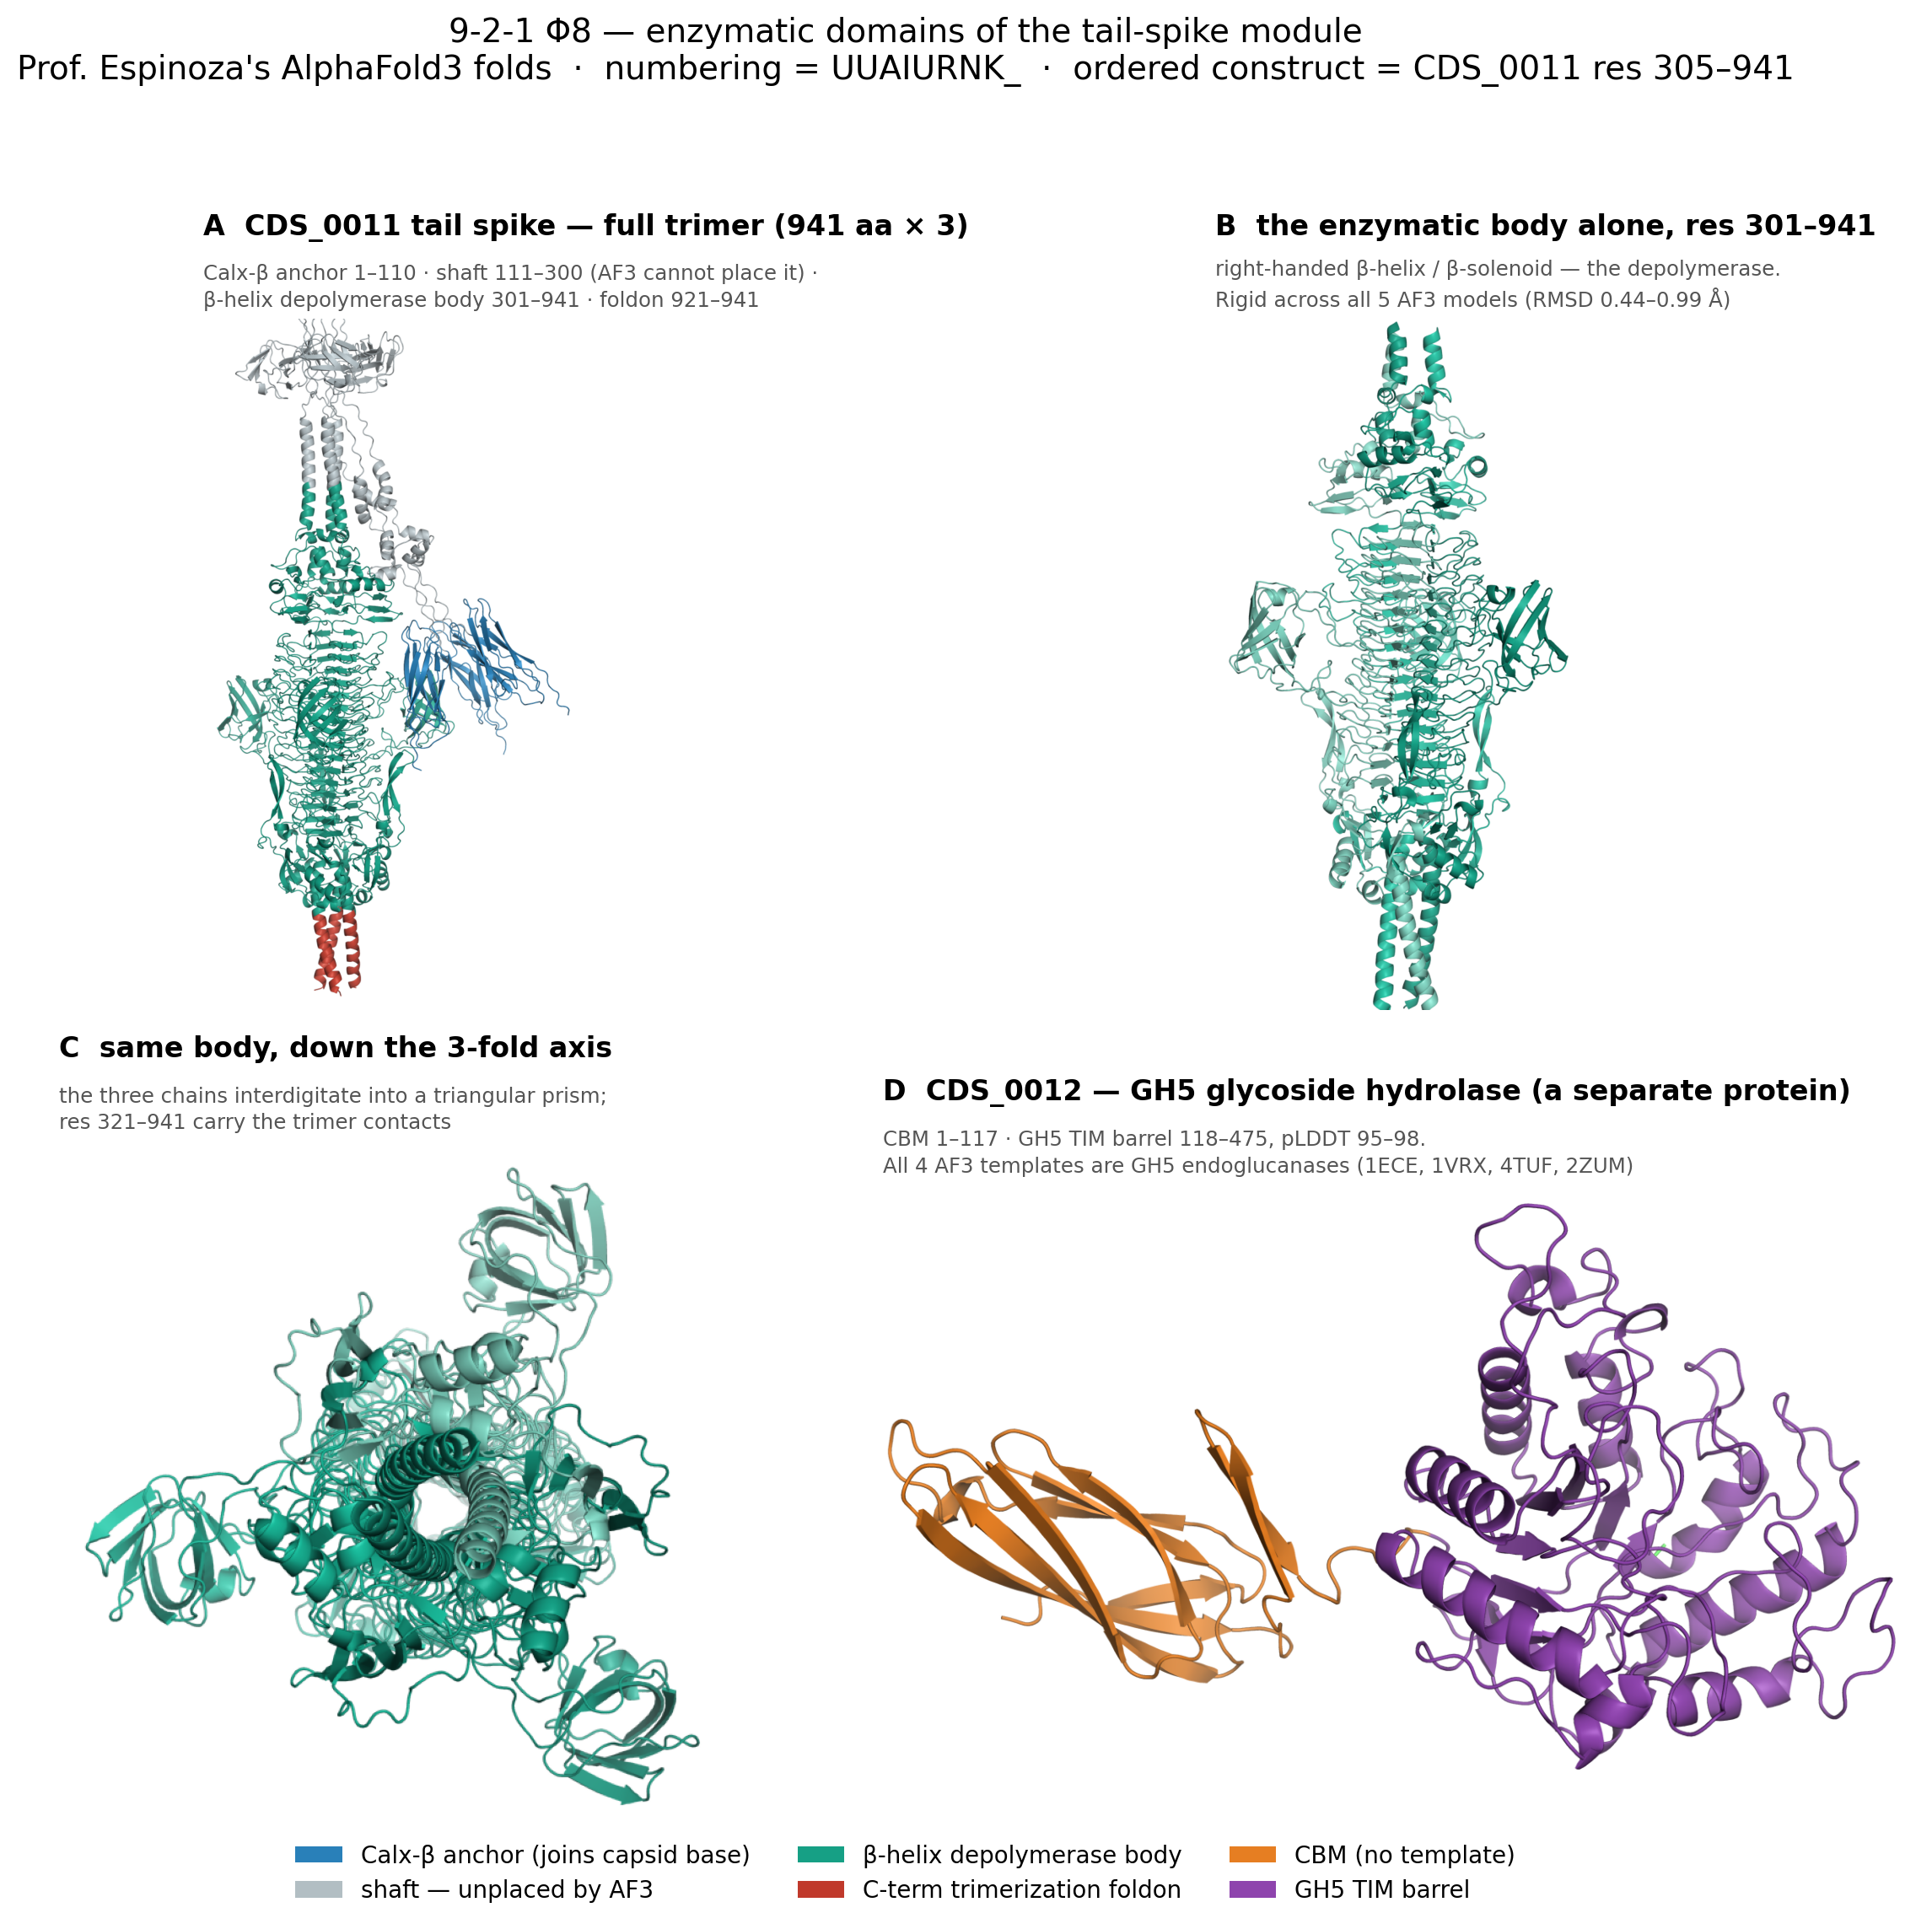
\includegraphics[width=0.68\textwidth,height=0.76\textheight,keepaspectratio]{../../code/output/0729_prof_figures/fig_enzymatic_domains.png}\\
  {\scriptsize\color{muted} Panel D is CDS\_0012 — a \textbf{separate protein}, not a domain of the
   tail spike.}
\end{frame}

\end{document}
"` prints the speaker script instead of the slides
\ifdefined\NOTESONLY \setbeameroption{show only notes}\setbeamerfont{note page}{size=\footnotesize} \fi

\begin{document}

% ---------------------------------------------------------------- 1. title
\begin{frame}[plain]
  \vspace{6pt}
  \begin{center}
    {\LARGE\bfseries Engineering the part that picks the host}\\[4pt]
    {\large Which gene, what it binds, where evolution comes in}
  \end{center}
  \vspace{4pt}
  \begin{center}
    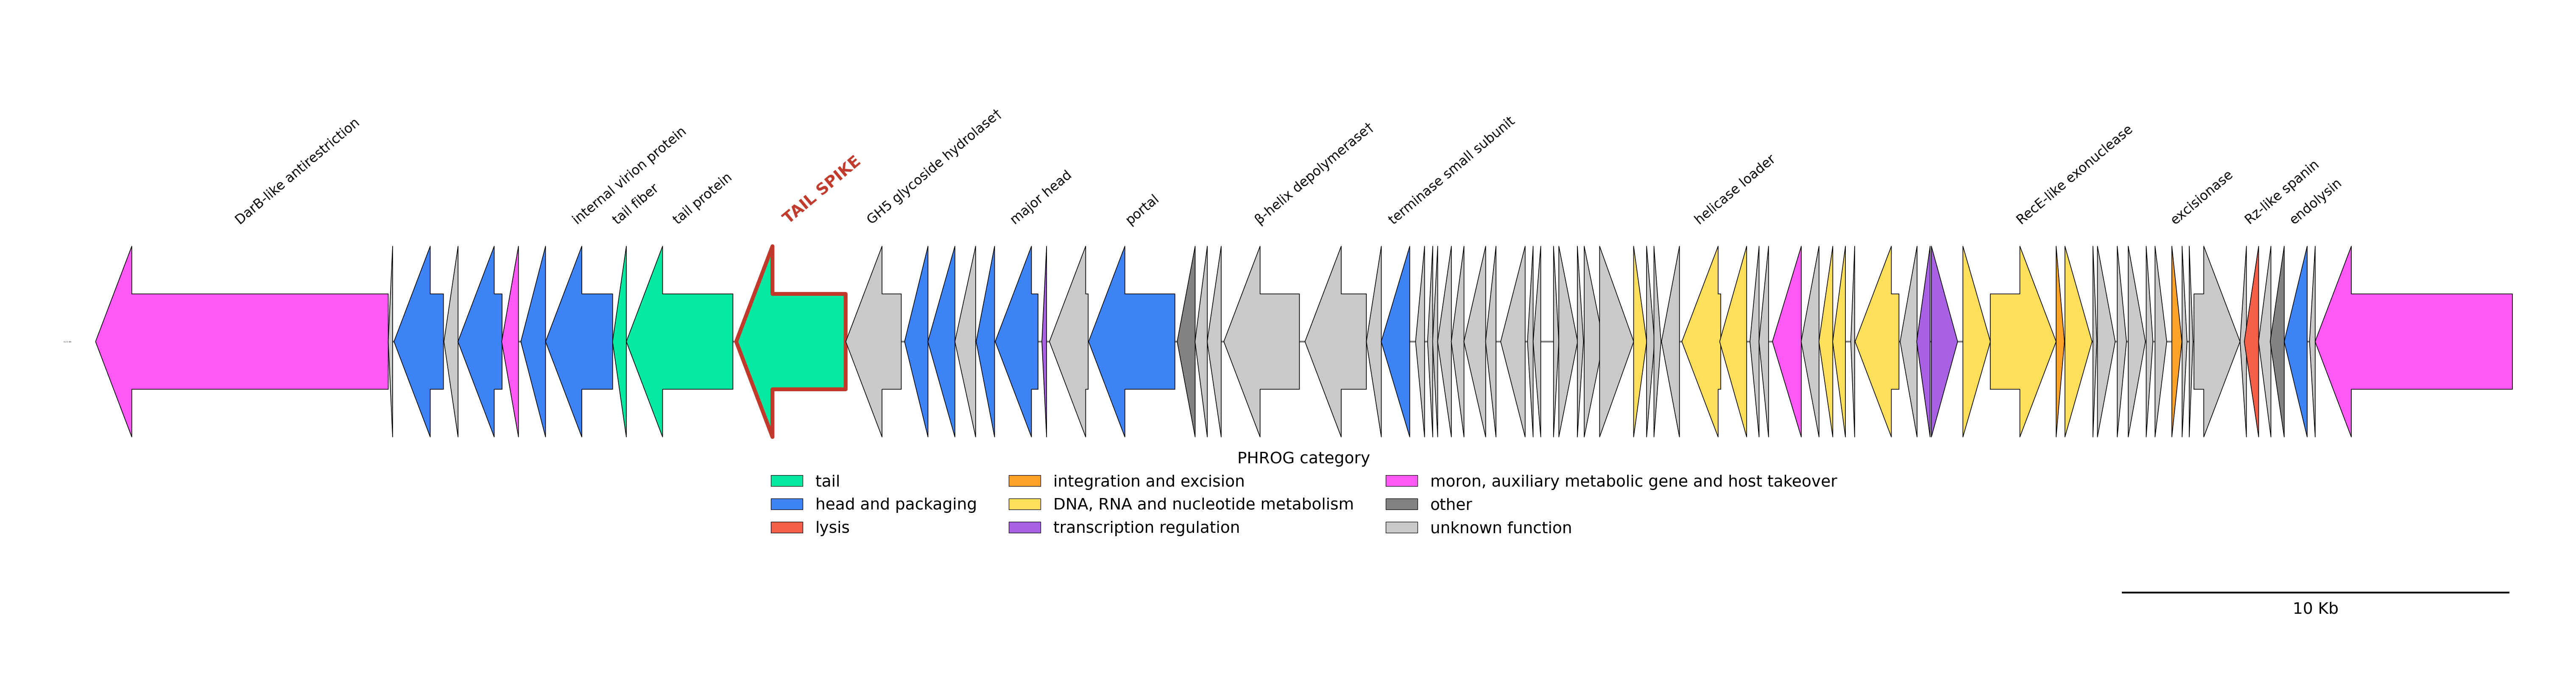
\includegraphics[width=0.95\textwidth]{fig/phage_map_banner.png}
  \end{center}
  \vspace{2pt}
  \begin{center}
  {\scriptsize\color{muted} Phage 9-2-1 $\Phi$8 — 62 kb, 80 genes — and three self-isolated
   \textit{Pseudomonas} strains\par
   \vspace{3pt}
   Chun-Yu (Alex) Chen \quad|\quad Phagenomics, Claremont CA \quad|\quad
   PI: J. Cesar Ignacio-Espinoza \quad|\quad 2026-08-21}
  \end{center}
  \note{
  Good evening. We are trying to build phage parts on purpose — to take the protein that decides which
  bacterium a phage can infect, and redesign it. Tonight: the two things you need before you can.\par
  ($\approx$18 s)}
\end{frame}

% ---------------------------------------------------------------- 2. context / goal
\begin{frame}[shrink=5]{We want to design the part, not just describe the phage}
  \begin{columns}[T,onlytextwidth]
    \begin{column}{0.53\textwidth}
      \footnotesize
      \begin{itemize}\setlength\itemsep{5pt}
        \item Phages hunt bacteria, and one phage usually infects \textbf{one strain} and ignores the
              next one over. Matching is done by \textbf{trial and error} today.
        \item Why now: \textcolor{cwzz}{\textbf{[AMR figure + source — Alex]}}. A phage is only useful
              if it hits the strain that is actually making someone sick.
        \item Our goal is a \textbf{part you can re-aim}: rebuild the receptor-binding protein so the
              same phage attacks a different strain.
        \item \textbf{We work on our own material} — local soil and water $\rightarrow$
              \textit{Pseudomonas} hosts and their phages, sequenced in house.
      \end{itemize}
      \vspace{4pt}
      \colorbox{accent!10}{\parbox{0.95\textwidth}{\centering\footnotesize
      \textbf{Tonight:} 5 isolates $\rightarrow$ \textbf{3 strains}, and one complete phage genome}}
    \end{column}
    \begin{column}{0.45\textwidth}
      \centering
      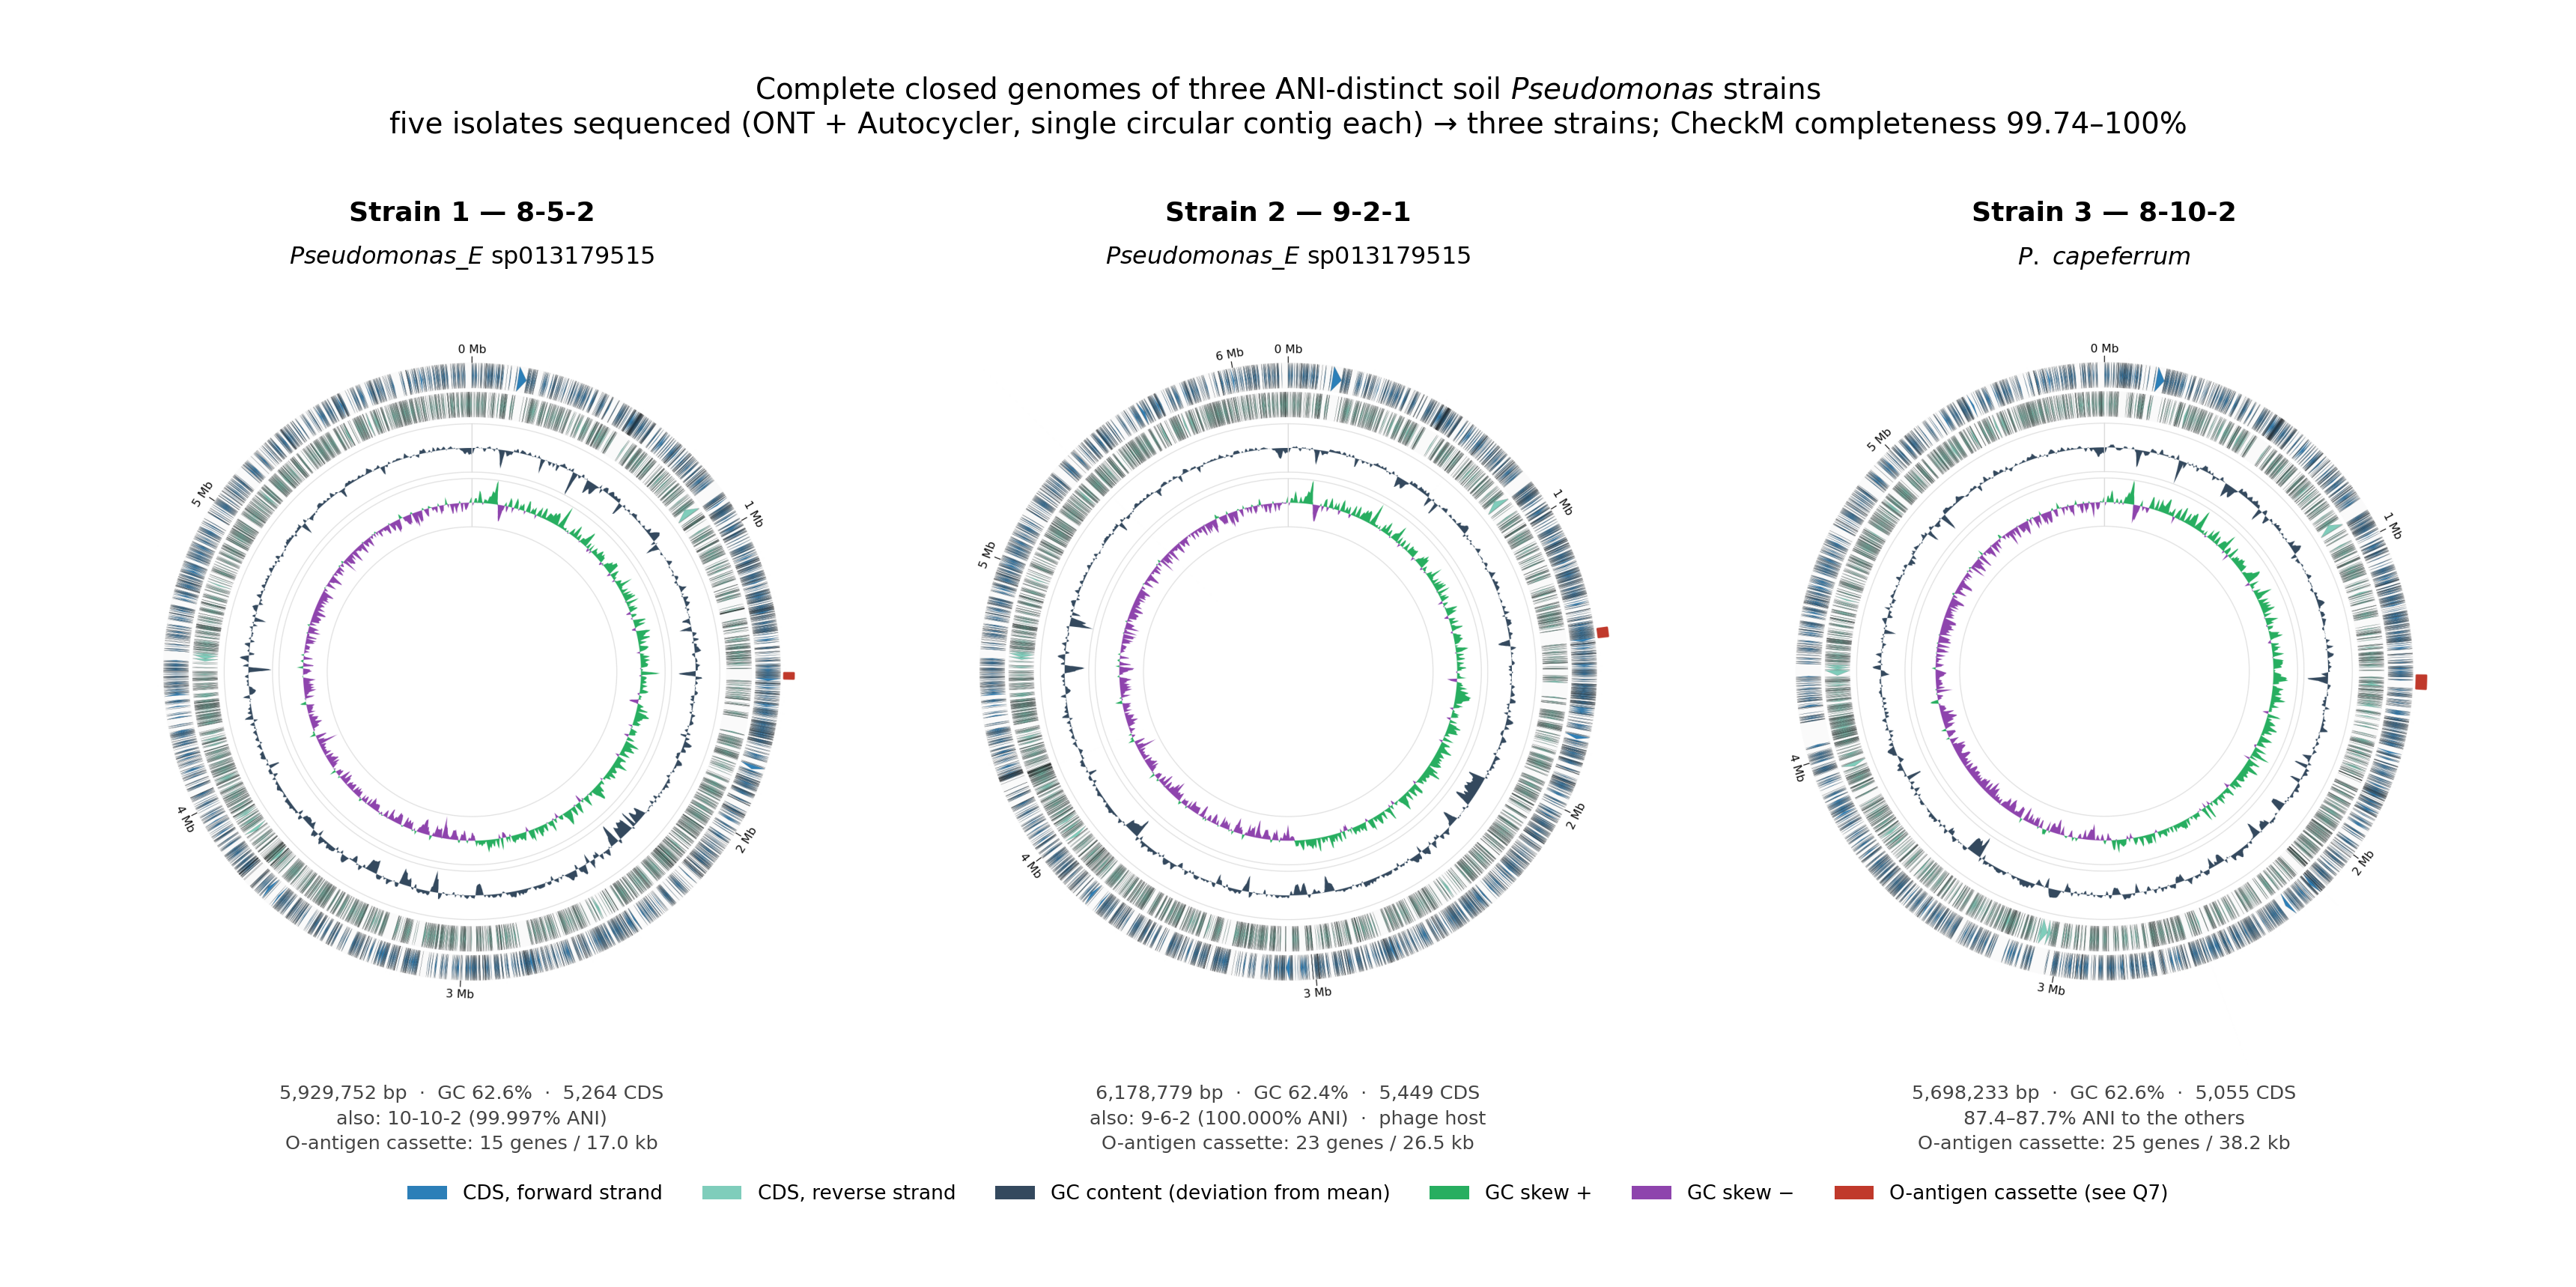
\includegraphics[width=0.98\textwidth]{../../code/output/0729_prof_figures/fig_bacterial_genomes.png}\\
      {\scriptsize\color{muted} three closed host genomes, 5.7–6.2 Mb}\\[5pt]
      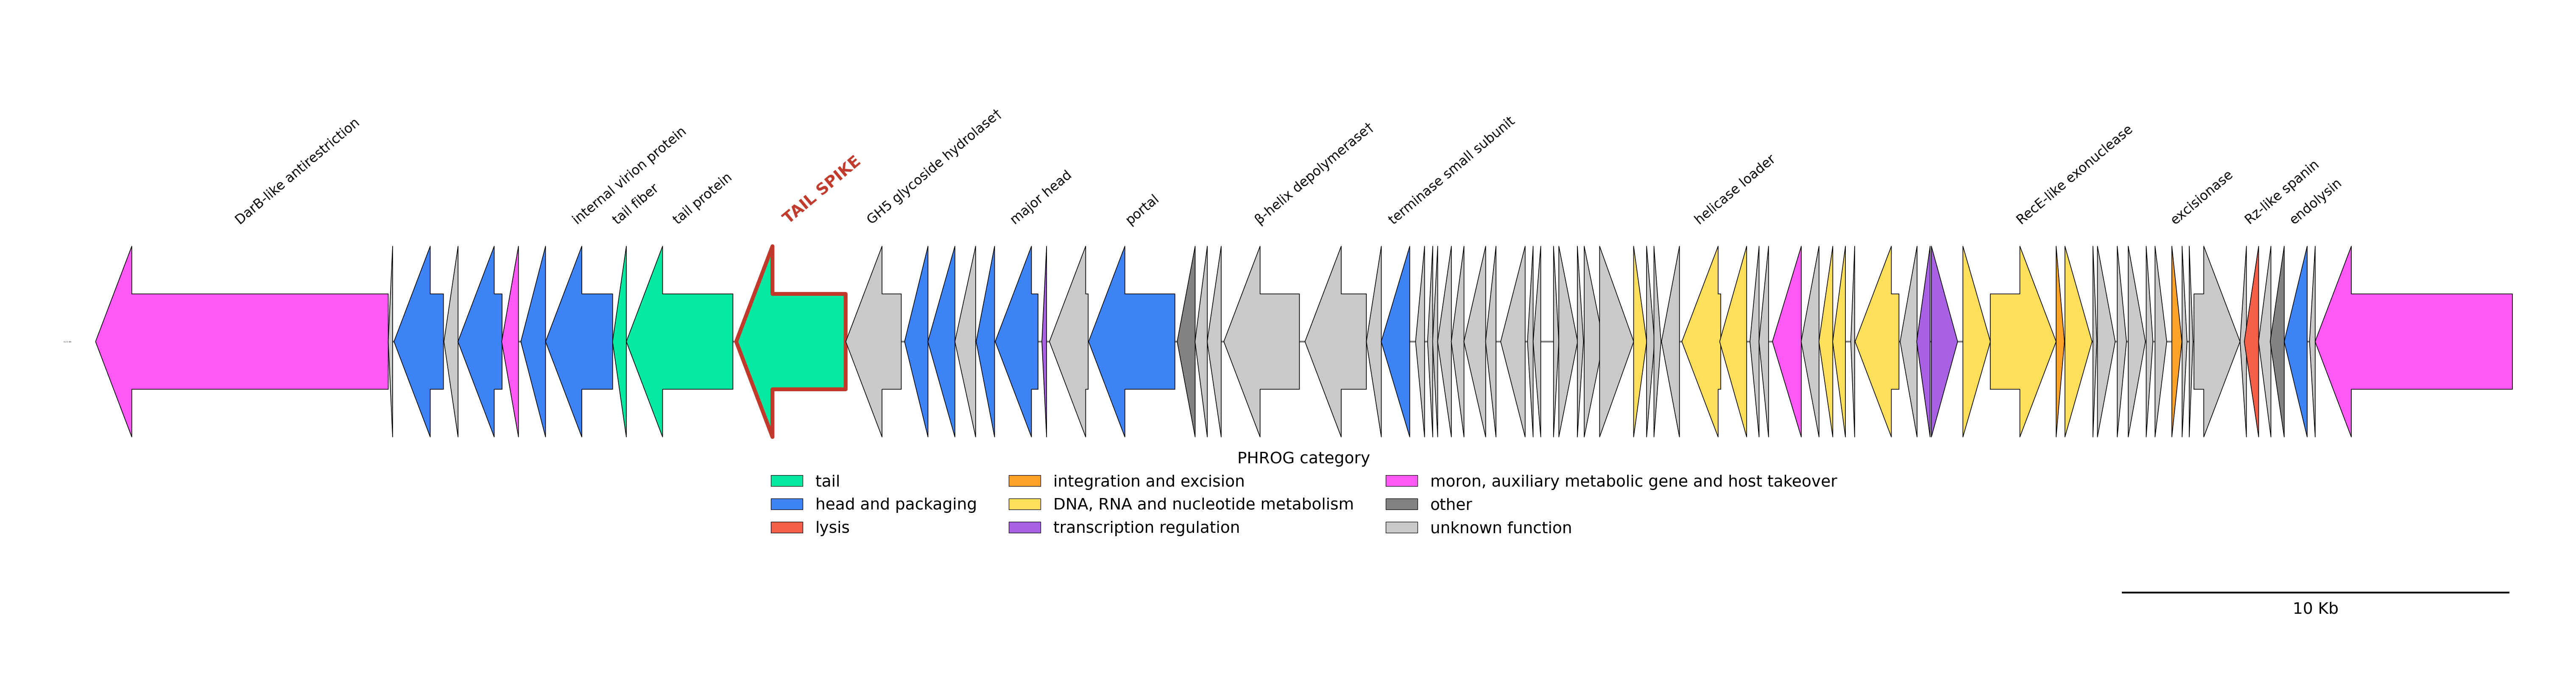
\includegraphics[width=0.98\textwidth]{fig/phage_map_banner.png}\\
      {\scriptsize\color{muted} the phage: 62 kb, 80 CDS, linear + 77 bp DTR}
    \end{column}
  \end{columns}
  \note{
  Phages hunt bacteria, and they are picky: one phage infects one strain and ignores the next one
  over. Today that match is trial and error.\par
  That matters right now — [AMR number, Alex fills in]. A phage is only useful if it hits the strain
  making someone sick.\par
  So our goal is not to describe a phage; it is to build a part you can re-aim — rebuild the
  receptor-binding protein so the same phage attacks a different strain.\par
  We work on our own material: local soil and water, Pseudomonas hosts and their phages, sequenced in
  house — five isolates, three strains, one complete phage genome.\par
  ($\approx$48 s)}
\end{frame}

% ---------------------------------------------------------------- 3. the design pipeline
\begin{frame}{The design loop — and where we actually are}
  \vspace{-2pt}
  \rqbox{Before you can redesign the targeting part: \textbf{which gene is it}, and \textbf{what must it recognise}?}
  \vspace{-2pt}
  \begin{center}
  \begin{tikzpicture}[
    font=\scriptsize,
    done/.style={draw=accent,line width=1.0pt,rounded corners=2pt,fill=accent!8,
                 text width=2.35cm,align=center,minimum height=1.8cm,inner sep=3pt},
    plan/.style={draw=muted,line width=0.9pt,dashed,rounded corners=2pt,fill=white,
                 text width=2.35cm,align=center,minimum height=1.8cm,inner sep=3pt},
    ar/.style={-{Stealth[length=4pt]},draw=muted,line width=0.7pt}]
    \node[done] (a) {\textbf{1. pick the gene}\\80 CDS $\rightarrow$ tail\\module: CDS\_0011,\\0012, 0024};
    \node[done,right=0.30cm of a] (b) {\textbf{2. define the\\target}\\fold it: what does\\it bind?};
    \node[plan,right=0.30cm of b] (c) {\textbf{3. learn from\\evolution}\\GH5 tree $\rightarrow$\\ancestral enzymes};
    \node[plan,right=0.30cm of c] (d) {\textbf{4. build\\variants}\\3 at Twist\\+ ancestral GH5};
    \node[plan,right=0.30cm of d] (e) {\textbf{5. test}\\fiber + depolymerase\\\emph{in trans}, 3 strains};
    \draw[ar] (a)--(b); \draw[ar] (b)--(c); \draw[ar] (c)--(d); \draw[ar] (d)--(e);
    \draw[ar,draw=muted,dashed] (e.south) -- ++(0,-0.35) -| node[pos=0.25,below,font=\scriptsize\color{muted}]{design rules} (c.south);
  \end{tikzpicture}
  \end{center}
  \vspace{2pt}
  {\scriptsize\color{muted} \tikz[baseline=-0.5ex]\draw[accent,line width=1pt,fill=accent!8] (0,0) rectangle (1.6ex,1.6ex);
   solid = has data \quad
   \tikz[baseline=-0.5ex]\draw[muted,dashed,line width=0.9pt] (0,0) rectangle (1.6ex,1.6ex);
   dashed = in progress / proposed \quad|\quad the next two slides are steps 1 and 2}
  \note{
  Here is the loop. Step one, pick the gene: of 80 genes the structural module narrows it to a
  handful — the tail spike, the GH5 beside it, and a depolymerase the annotator missed.\par
  Step two, define the target — you cannot redesign a binder without knowing what it binds.\par
  Step three is where evolution comes in. The tail spike decides who is recognised; the depolymerase
  decides what can be cut open. So we build a tree over all GH5 sequences and reconstruct ancestral
  enzymes — proteins from different points in evolution, not random mutants. Stated caveat: this
  assumes affinity tracks infection.\par
  Step four, build them: three constructs are at Twist, ancestral enzymes next. Step five, combine
  fiber and depolymerase in trans on our three strains, and feed that back as design rules.\par
  Solid boxes have data; dashed ones do not. The next two slides are steps one and two.\par
  ($\approx$62 s)}
\end{frame}

% ---------------------------------------------------------------- 4. result 1 — the part
\begin{frame}[shrink=5]{Steps 1--2: a $\beta$-helix depolymerase — the target is a sugar}
  \begin{columns}[T,onlytextwidth]
    \begin{column}{0.30\textwidth}
      \centering
      \includegraphics[height=0.60\textheight]{../../code/output/0729_prof_figures/panels/cds0011_trimer_domains.png}\\[2pt]
      {\scriptsize\color{muted} CDS\_0011 trimer, 941 aa $\times$ 3\par
       grey shaft \textbullet\ blue anchor\par
       \textcolor{accent}{\textbf{teal body}} \textbullet\ red foldon}
    \end{column}
    \begin{column}{0.68\textwidth}
      \footnotesize
      \begin{itemize}\setlength\itemsep{5pt}
        \item Right-handed \textbf{$\beta$-helix}, one rung every \textbf{15–18 residues} — the
              signature of a polysaccharide depolymerase. \textbf{This part cuts sugar}, so its target
              is the surface sugar, not a protein.
        \item The domain map is what makes it \textbf{engineerable}: pLDDT 88–94, and the body
              (res 301–941) is rigid to \textbf{0.44–0.99 \AA} across five models — that boundary is
              exactly where our construct starts (res 305).
        \item The protein--protein hypothesis was tested first \textbf{and failed}:
      \end{itemize}
      \vspace{1pt}
      \begin{center}
        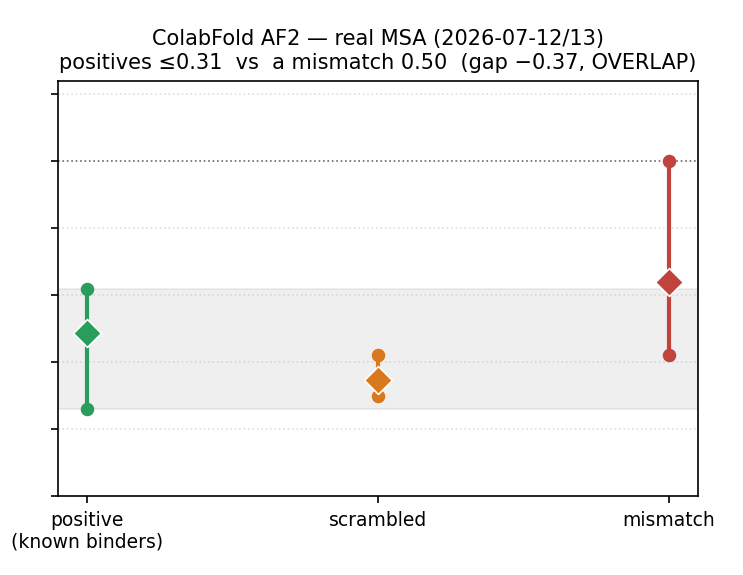
\includegraphics[height=0.25\textheight]{fig/binding_controls_af2.png}\\
        {\scriptsize\color{muted} positives ipTM $\leq$ 0.31 vs a mismatched pair 0.50 — no signal}
      \end{center}
    \end{column}
  \end{columns}
  \note{
  Steps one and two on one slide. This is the tail spike, 941 residues, a trimer: grey shaft AlphaFold
  cannot place, blue anchor into the capsid, teal working body.\par
  That body is a right-handed beta helix, one rung every 15 to 18 residues — the signature of a
  depolymerase. So the part cuts sugar, and its target is the surface sugar, not a protein.\par
  It is also engineerable: the body from residue 301 is rigid, under one angstrom across five models,
  and that boundary is exactly where our construct starts.\par
  And we tested the protein-protein hypothesis first — docking gave positives at 0.31 and a mismatch
  at 0.50. No discriminating power, so we retired that screen.\par
  ($\approx$57 s)}
\end{frame}

% ---------------------------------------------------------------- 5. result 2 — the target varies
\begin{frame}[shrink=5]{The target is different in every strain — that is the handle}
  \vspace{1pt}
  \footnotesize Same \texttt{ihfB}-flanked slot, different cargo
   \ \textcolor{muted}{(grey ribbons = homology)}\normalsize
  \vspace{1pt}
  \begin{center}
    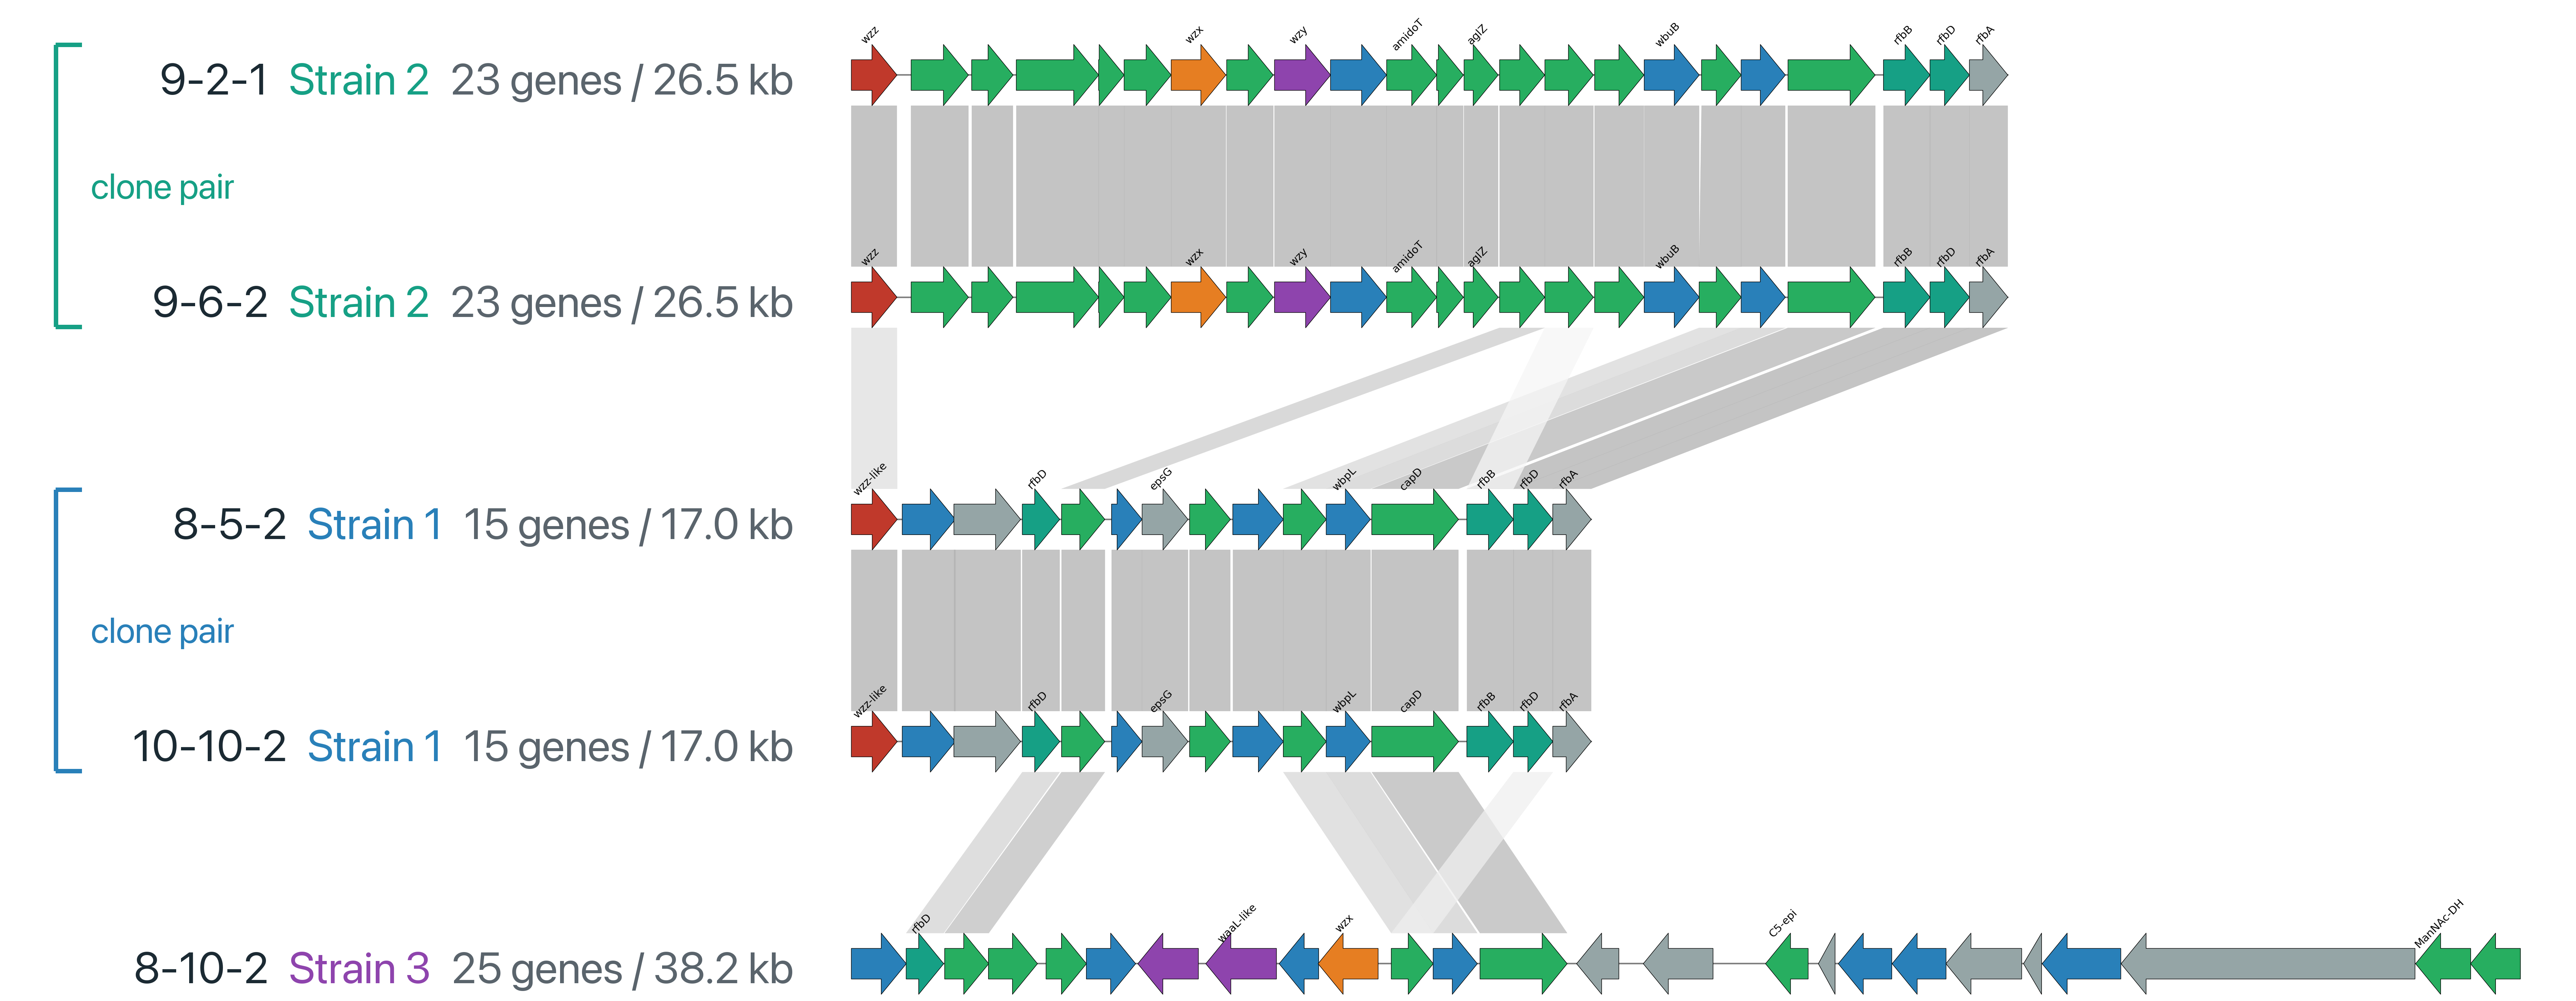
\includegraphics[width=0.95\textwidth,height=0.54\textheight,keepaspectratio]{fig/oantigen_tracks_labeled.png}
  \end{center}
  \vspace{-4pt}
  \begin{center}\tiny
    \chip{cwzz}{chain-length regulator}\quad\chip{cwzx}{flippase (wzx)}\quad\chip{cwzy}{polymerase (wzy)}\quad
    \chip{cgt}{glycosyltransferase}\quad\chip{crha}{dTDP-rhamnose}\quad\chip{cnuc}{nucleotide-sugar}\quad
    \chip{cother}{unassigned}
  \end{center}
  \vspace{1pt}
  {\footnotesize \textbf{4 of 45 clusters shared by all three} — generic sugar chemistry only, no
   shared assembly machinery. \textcolor{muted}{Control: clone pairs 100.0\% identical.}}
  \note{
  If the part reads a sugar, does that sugar differ between strains? That difference is the handle a
  redesigned part would turn.\par
  Five tracks: two Strain 2 clones, two Strain 1 clones, Strain 3; arrows are genes, grey ribbons are
  homology. Control first: inside each clone pair all 23 and all 15 genes are identical. ANI
  saturates, so this had to be measured.\par
  Across strains the links are sparse and crossed — of 45 clusters only four are shared, all generic
  sugar chemistry, no shared flippase, polymerase or chain-length regulator.\par
  Three strains, three targets. This phage should not plaque on the other two, and a re-aimed part is
  what would change that.\par
  ($\approx$57 s)}
\end{frame}

% ---------------------------------------------------------------- 6. close
\begin{frame}[shrink=5]{Where the loop stands}
  \begin{columns}[T,onlytextwidth]
    \begin{column}{0.50\textwidth}
      \small
      \textcolor{accent}{\textbf{Conclusion}}\\
      We know \textbf{which gene} to engineer and \textbf{what it must recognise}: the tail-spike
      depolymerase, against a strain-specific O-antigen — and our three strains give three different
      targets.
      \vspace{6pt}

      \textcolor{accent}{\textbf{Limitation}}\\
      Steps 3–5 are \textbf{not results yet}: the GH5 ancestral reconstruction is still being built,
      the constructs are not expressed, and the cross-strain plaque assay was run July 4 but the data
      is not in our hands. It also assumes affinity tracks infection. No serotyping tool exists for
      this taxon, so we cannot name an O-type.
      \vspace{6pt}

      \textcolor{accent}{\textbf{Next three months}}\\
      Recover that readout; express the three constructs; reconstruct ancestral GH5 enzymes and test
      fiber $+$ depolymerase \emph{in trans} on the three strains. The tail spike also has a
      15,775-sequence alignment — enough for a conservation profile on the structure.
    \end{column}
    \begin{column}{0.48\textwidth}
      \centering
      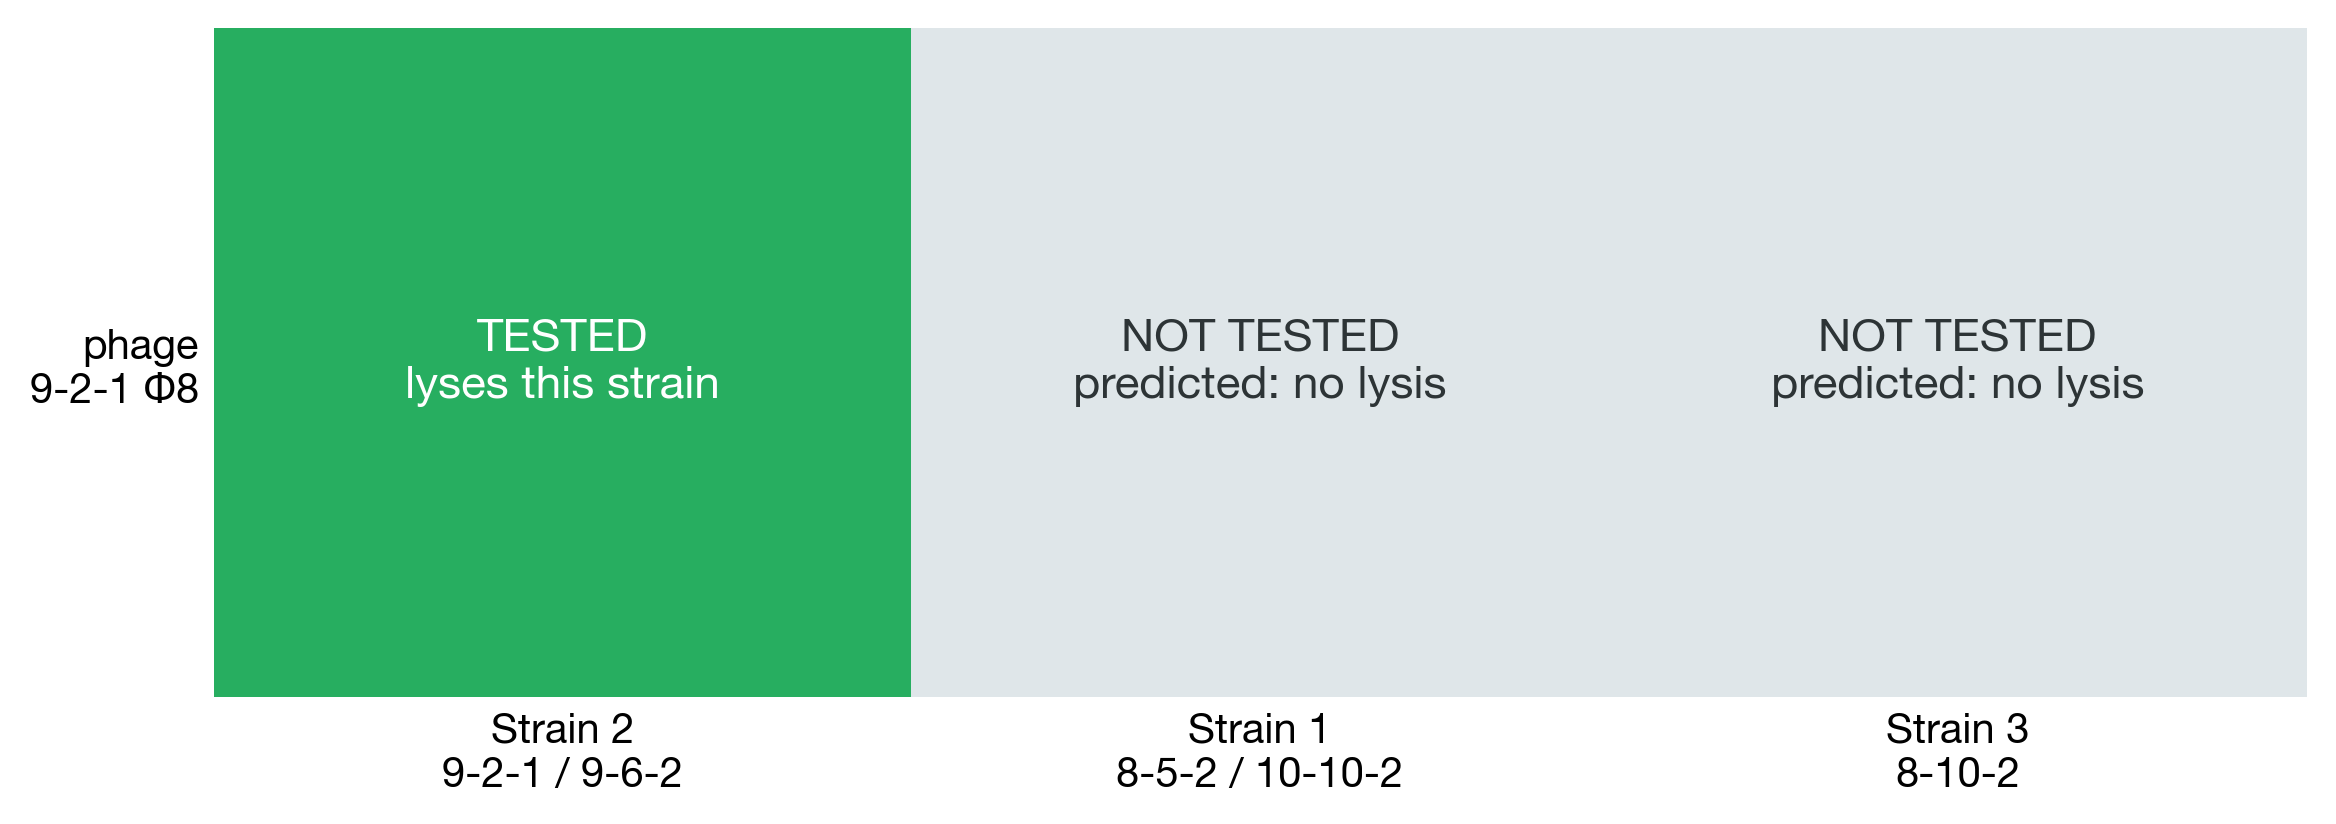
\includegraphics[width=\textwidth]{fig/hostrange_cells.png}\\[3pt]
      {\scriptsize\color{muted} only Strain 2 has actually been challenged; the grey cells are
       predictions, and the July 4 assay reads them out}\\[8pt]
      \begin{flushleft}\scriptsize
      \textcolor{accent}{\textbf{1. pick the gene}} — done\\
      \textcolor{accent}{\textbf{2. define the target}} — done\\
      \textcolor{muted}{\textbf{3. ancestral GH5 enzymes} — PI building the tree}\\
      \textcolor{muted}{\textbf{4. build} — 3 constructs at Twist}\\
      \textcolor{muted}{\textbf{5. test} — \emph{in trans}, waiting on the July 4 readout}
      \end{flushleft}
    \end{column}
  \end{columns}
  \vspace{5pt}
  \begin{center}\large\bfseries We now know which part to rebuild and what it has to grip — the
   ancestral variants are the next lever.\end{center}
  \note{
  Where the loop stands. We know which gene to engineer and what it must recognise — the tail-spike
  depolymerase against a strain-specific O-antigen — and three strains give three targets.\par
  The limitation is honest: steps three to five are not results — the GH5 tree is still being built,
  the constructs are not expressed, and the July fourth plaque data is not in our hands. And no
  serotyping tool exists for this taxon, so we cannot name an O-type.\par
  Next three months: recover that readout, express the constructs, and reconstruct ancestral GH5
  enzymes — then measure how proteins from different points in evolution behave with the fiber, in
  trans, on the three strains.\par
  We know which part to rebuild and what it has to grip. The ancestral variants are the next lever.\par
  ($\approx$58 s — stop here, not on a thank-you slide)}
\end{frame}

% ================================================================ backup
\begin{frame}[plain]
  \vspace{1.2cm}\centering{\Large\bfseries Backup}\\[4pt]{\color{muted} not shown unless asked}
\end{frame}

\begin{frame}{Backup 1 — gene selection and the constructs}
  \small
  \begin{itemize}\setlength\itemsep{5pt}
    \item Structural module, in canonical podovirus order: portal (CDS\_0020) $\rightarrow$ major
          capsid (0017) $\rightarrow$ adaptors $\rightarrow$ \textbf{tail spike (0011)} $\rightarrow$
          tail (0010) $\rightarrow$ fiber (0009).
    \item \textbf{CDS\_0024 is a second $\beta$-helix depolymerase} (rung 22–24) that Pharokka called
          ``hypothetical''; the de-novo RBP classifier found it at score 0.998.
    \item \textbf{CDS\_0012 is a GH5 glycoside hydrolase} — a separate protein, not a domain of the
          tail spike; all four AF3 templates are GH5 endoglucanases.
    \item Ordered from Twist 2026-07-27, all in pET-28a(+) with N-terminal His6:
          CDS\_0011 res \textbf{305–941} (the rigid body), CDS\_0010 res 105–917,
          CDS\_0012 res 117–477.
    \item CDS\_0010 is an \textbf{unknown protein} — the glycosidase call was withdrawn 2026-07-29;
          it is being expressed for functional characterisation.
  \end{itemize}
\end{frame}

\begin{frame}{Backup 2 — how the locus was pulled, how orthology was called}
  \small
  \begin{itemize}\setlength\itemsep{5pt}
    \item Anchor, identical in all five genomes: 30S ribosomal protein S1 $\rightarrow$ \texttt{ihfB}
          $\rightarrow$ LPS assembly protein A $\rightarrow$ MBL-fold hydrolase $\rightarrow$
          \textbf{cassette starts}. \texttt{ihfB} is the canonical upstream flank of the
          \textit{Pseudomonas} OSA cluster in the literature.
    \item Orthology = MMseqs2 clustering, $\geq$30\% identity / $\geq$50\% coverage.
          \textbf{Product names cannot be used}: the chain-length regulators of Strain 1 and Strain 2
          carry different Bakta labels but are homologous by sequence.
    \item Locus sizes: Strain 2 = 23 genes / 26.5 kb \textbullet\ Strain 1 = 15 / 17.0 kb \textbullet\
          Strain 3 = 25 / 38.2 kb.
    \item The cross-strain best-hit numbers (9/23, 10/23, 6/15) are one-directional best hits at a
          looser cutoff and are not meant to reconcile with the 45/4 cluster counts.
  \end{itemize}
\end{frame}

\begin{frame}{Backup 3 — cluster matrix, 45 clusters $\times$ 3 strains}
  \centering
  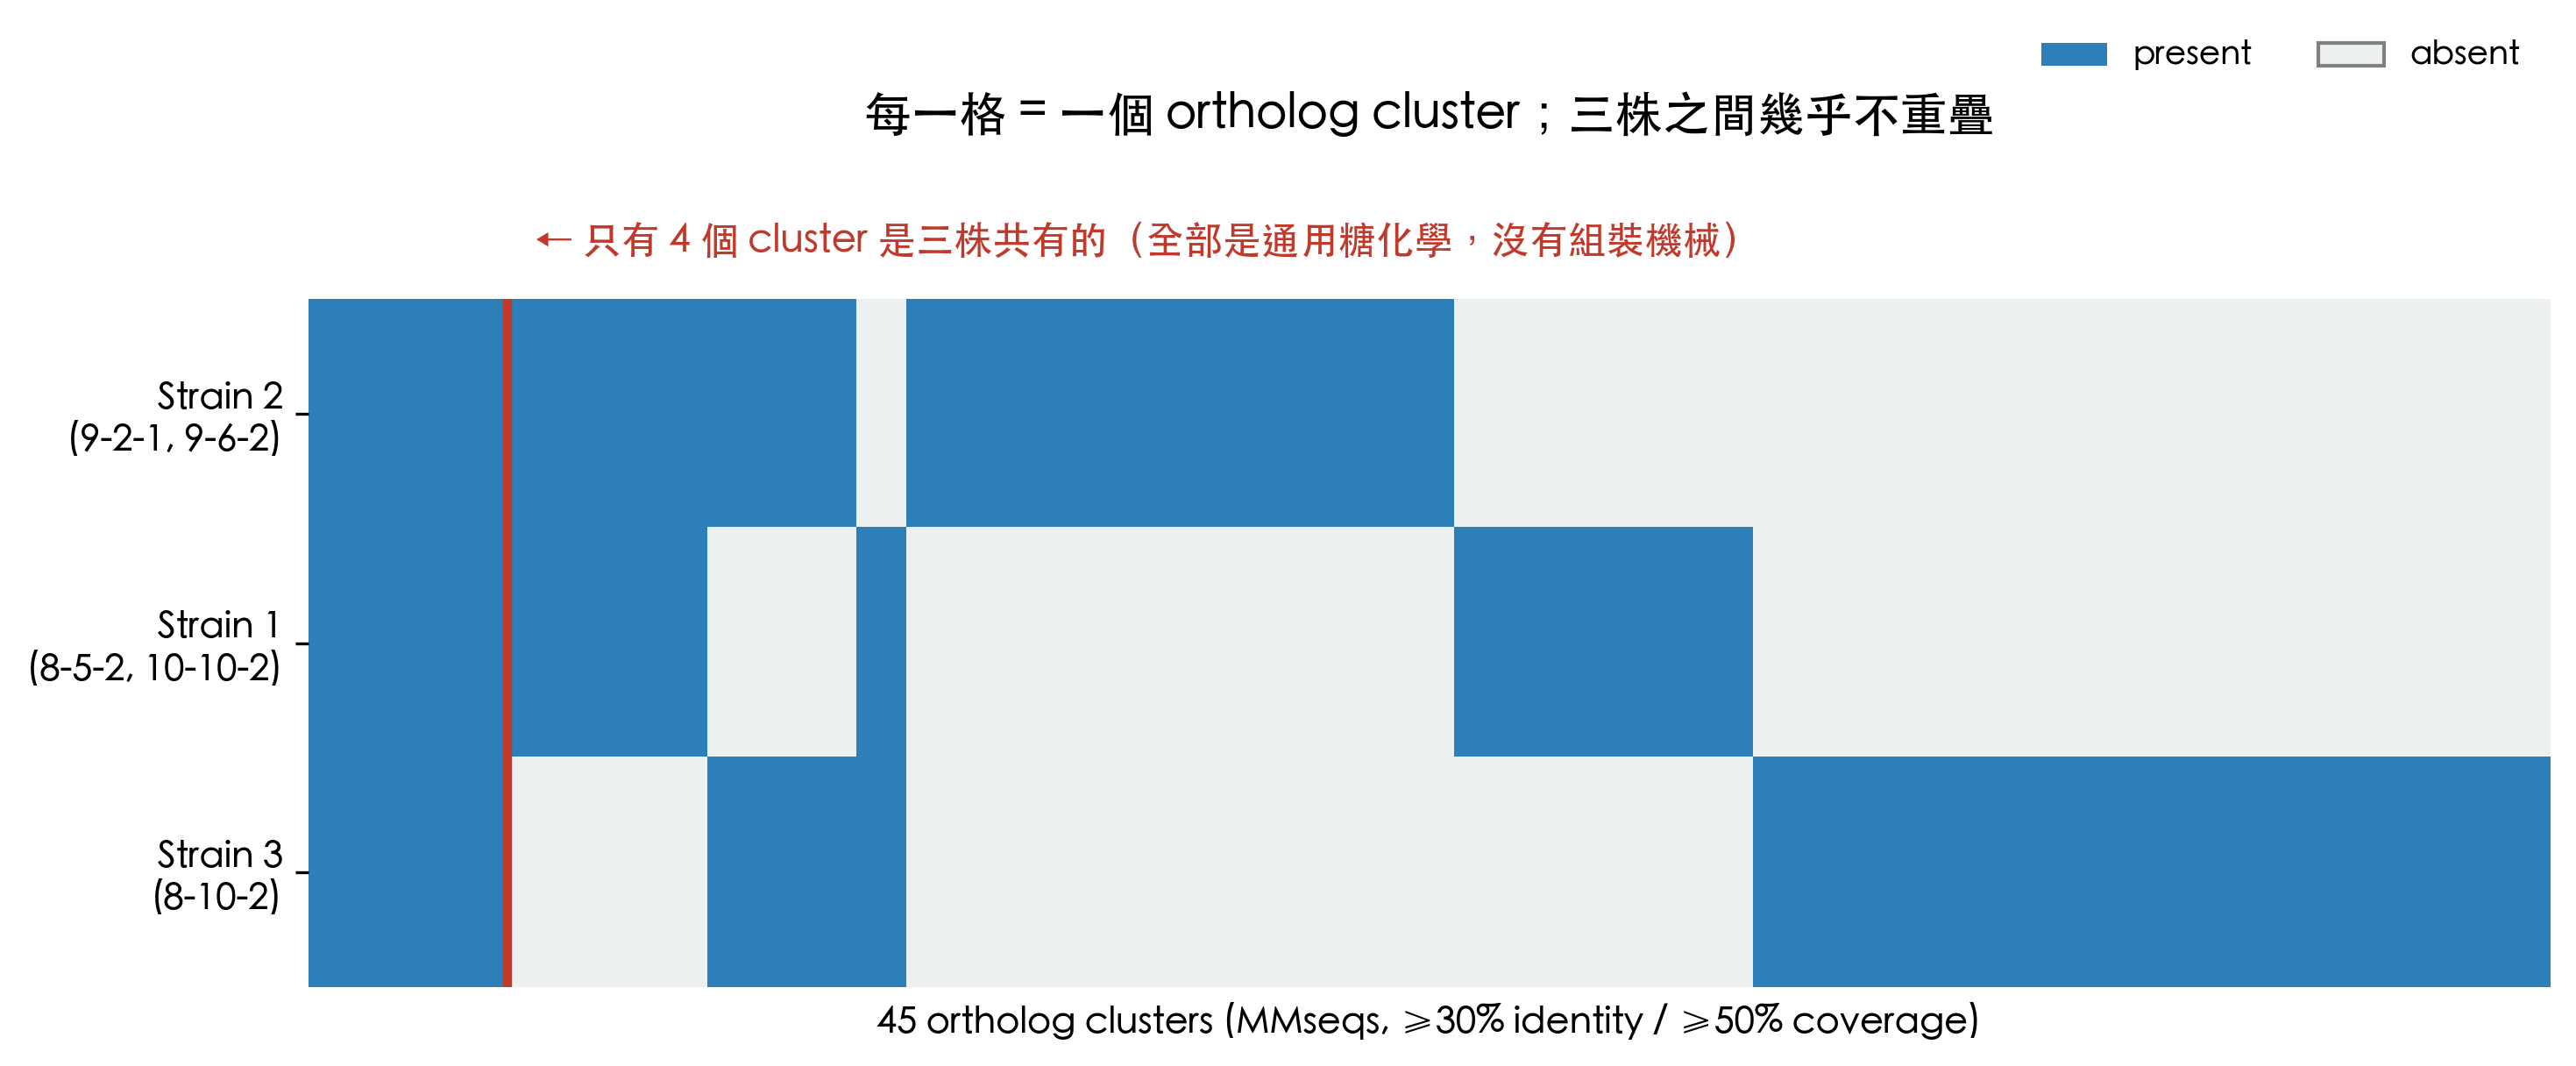
\includegraphics[width=0.86\textwidth,height=0.74\textheight,keepaspectratio]{../../code/output/0727_o_antigen_comparison/fig2_cluster_presence.png}
\end{frame}

\begin{frame}{Backup 4 — limitations in full}
  \small
  \begin{itemize}\setlength\itemsep{5pt}
    \item \textbf{Variable $\neq$ specificity-determining.} An earlier plan to read specificity off
          metagenomic variable regions was rejected in our own review: metagenome sequences carry no
          host labels, so specificity-determining positions cannot be identified that way. The
          15,775-sequence alignment (tail spike, CDS\_0011) supports a \textbf{conservation profile}
          — not ``these residues set the host range''. The ancestral reconstruction the PI is building
          is a separate thing: a tree over \textbf{all GH5 sequences} (CDS\_0012), whose ancestral
          enzymes get expressed and challenged \emph{in trans}, under the stated caveat that
          affinity $\sim$ binding $\sim$ infection.
    \item \textbf{Do not say Strain 1 lacks a flippase or polymerase} — Bakta assigns no Pfam/InterPro
          to those two genes; confirming them needs InterProScan.
    \item \textbf{The sugar structure has not been measured} — gene content is not structure; that
          needs LPS extraction and mass spectrometry.
    \item \textbf{The $\beta$-helix has no named structural homolog yet} — no foldseek or DALI run.
    \item \textbf{Taxonomy}: the virion module is podovirus-like, but reciprocal best hits against T7,
          $\varphi$KMV and KP32 are $\approx$0 and the genome carries an excisionase; \textit{terL} is
          unannotated, so formal taxonomy cannot be run. ``T7-like'' is an organizational analogy only.
  \end{itemize}
\end{frame}

\begin{frame}{Backup 5 — the three host genomes}
  \centering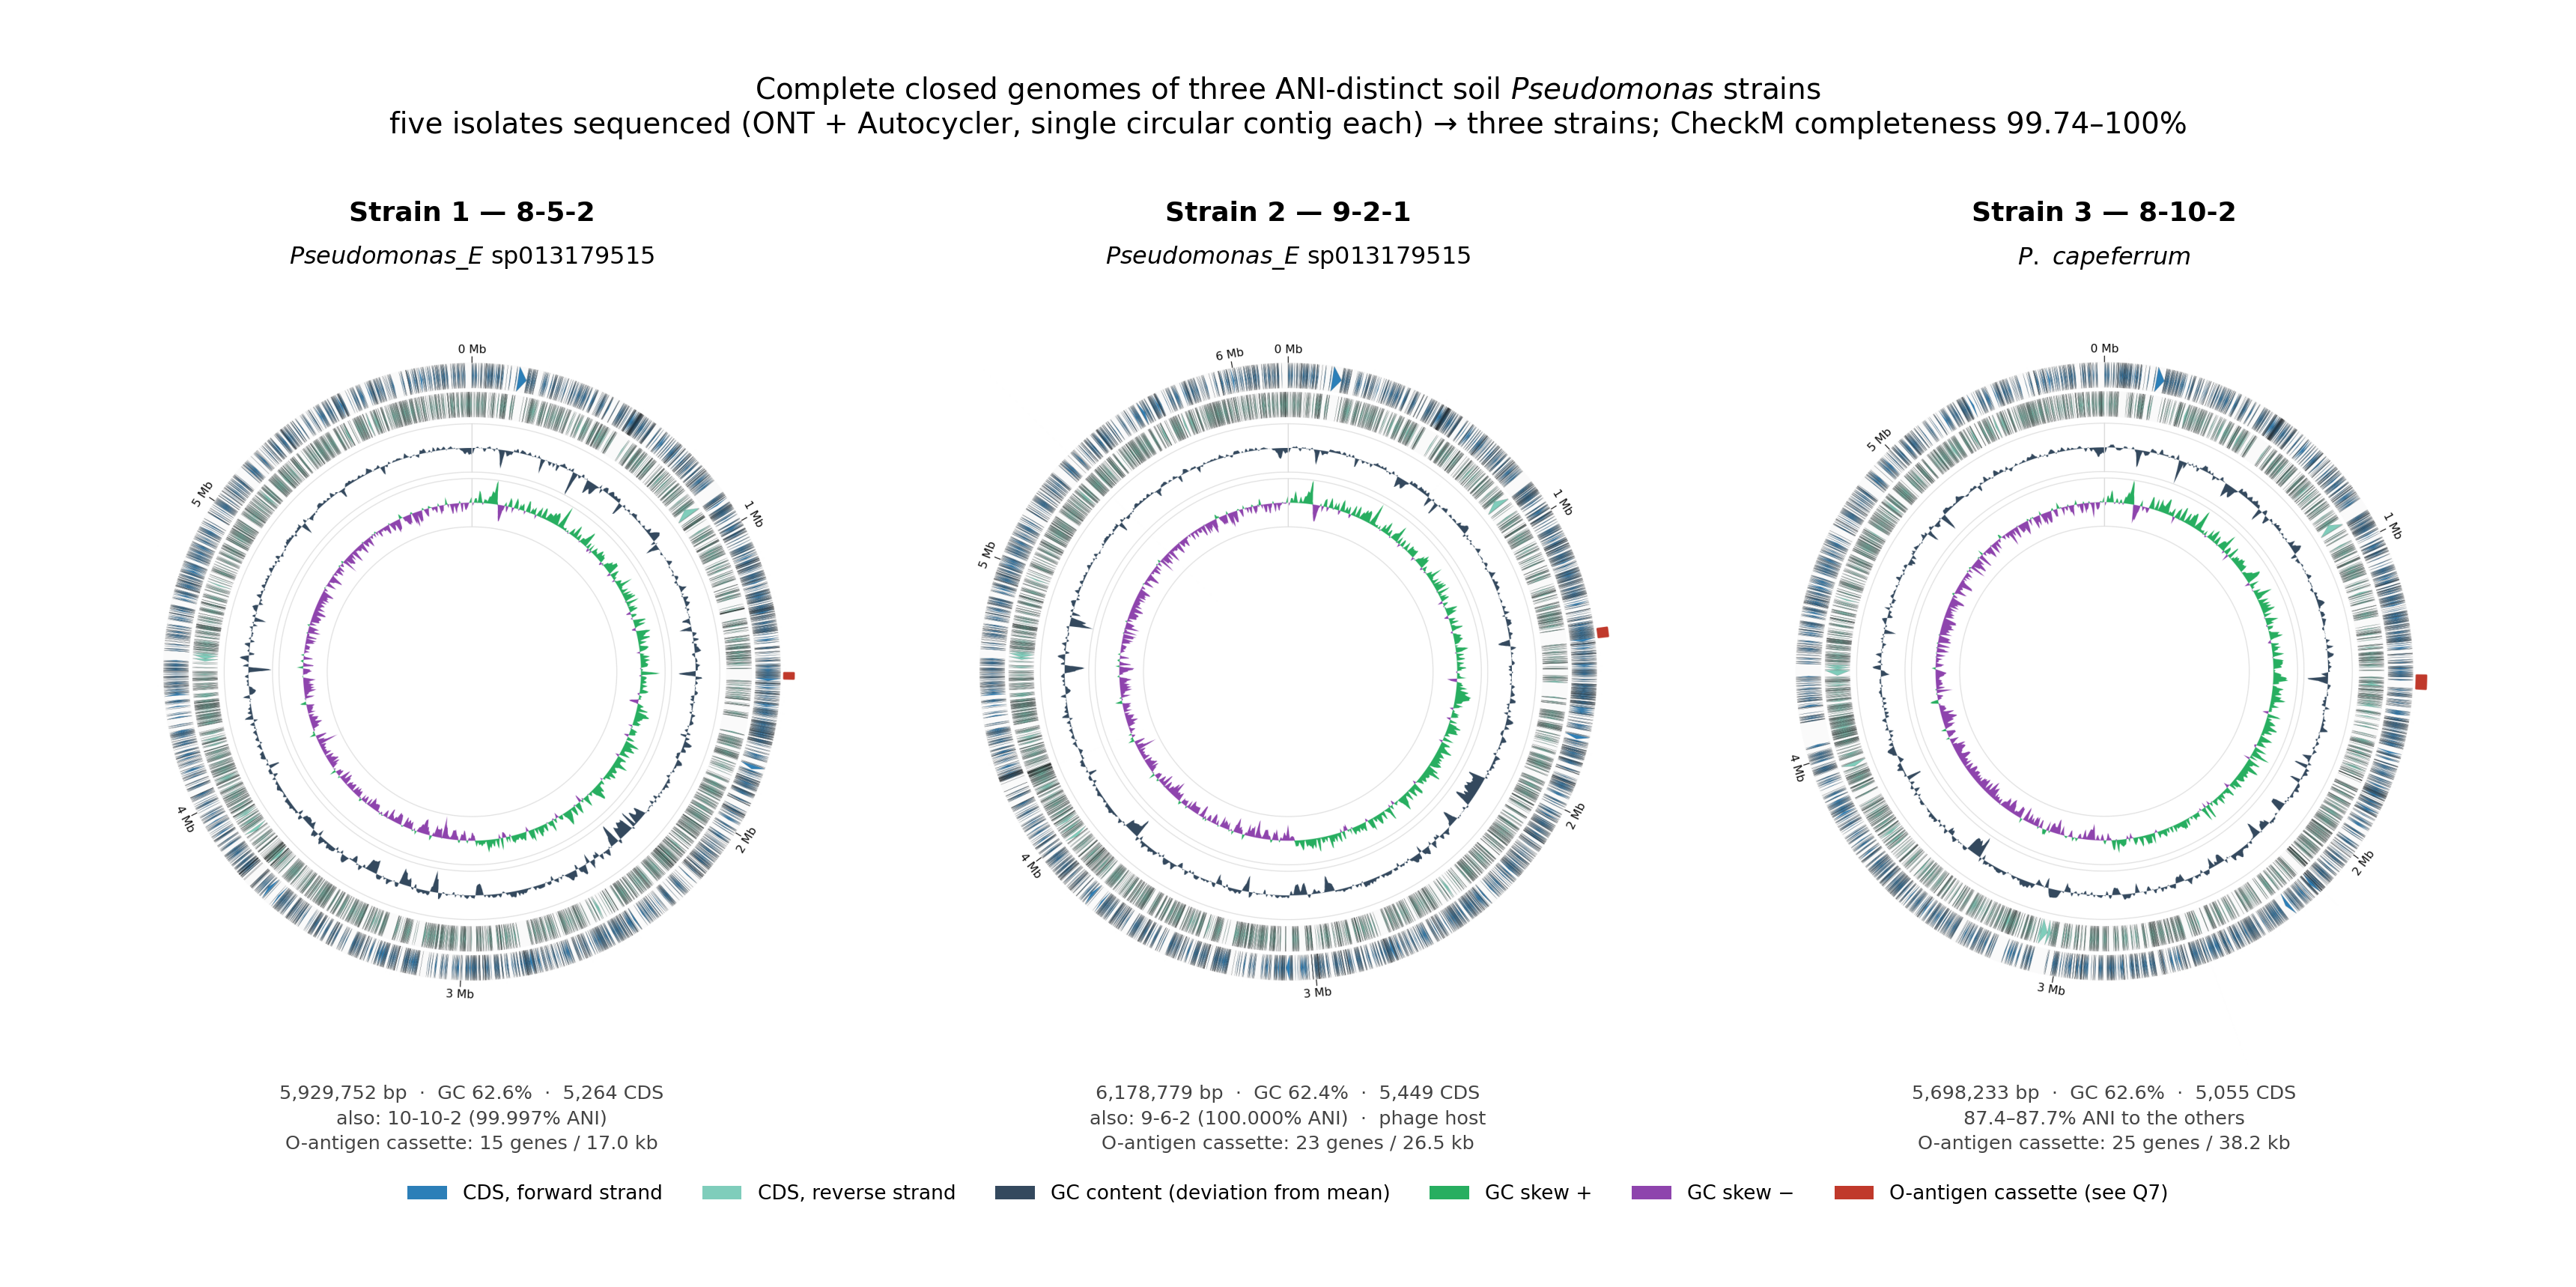
\includegraphics[width=0.95\textwidth,height=0.78\textheight,keepaspectratio]{../../code/output/0729_prof_figures/fig_bacterial_genomes.png}
\end{frame}

\begin{frame}{Backup 6 — phage genome, tail / RBP module}
  \centering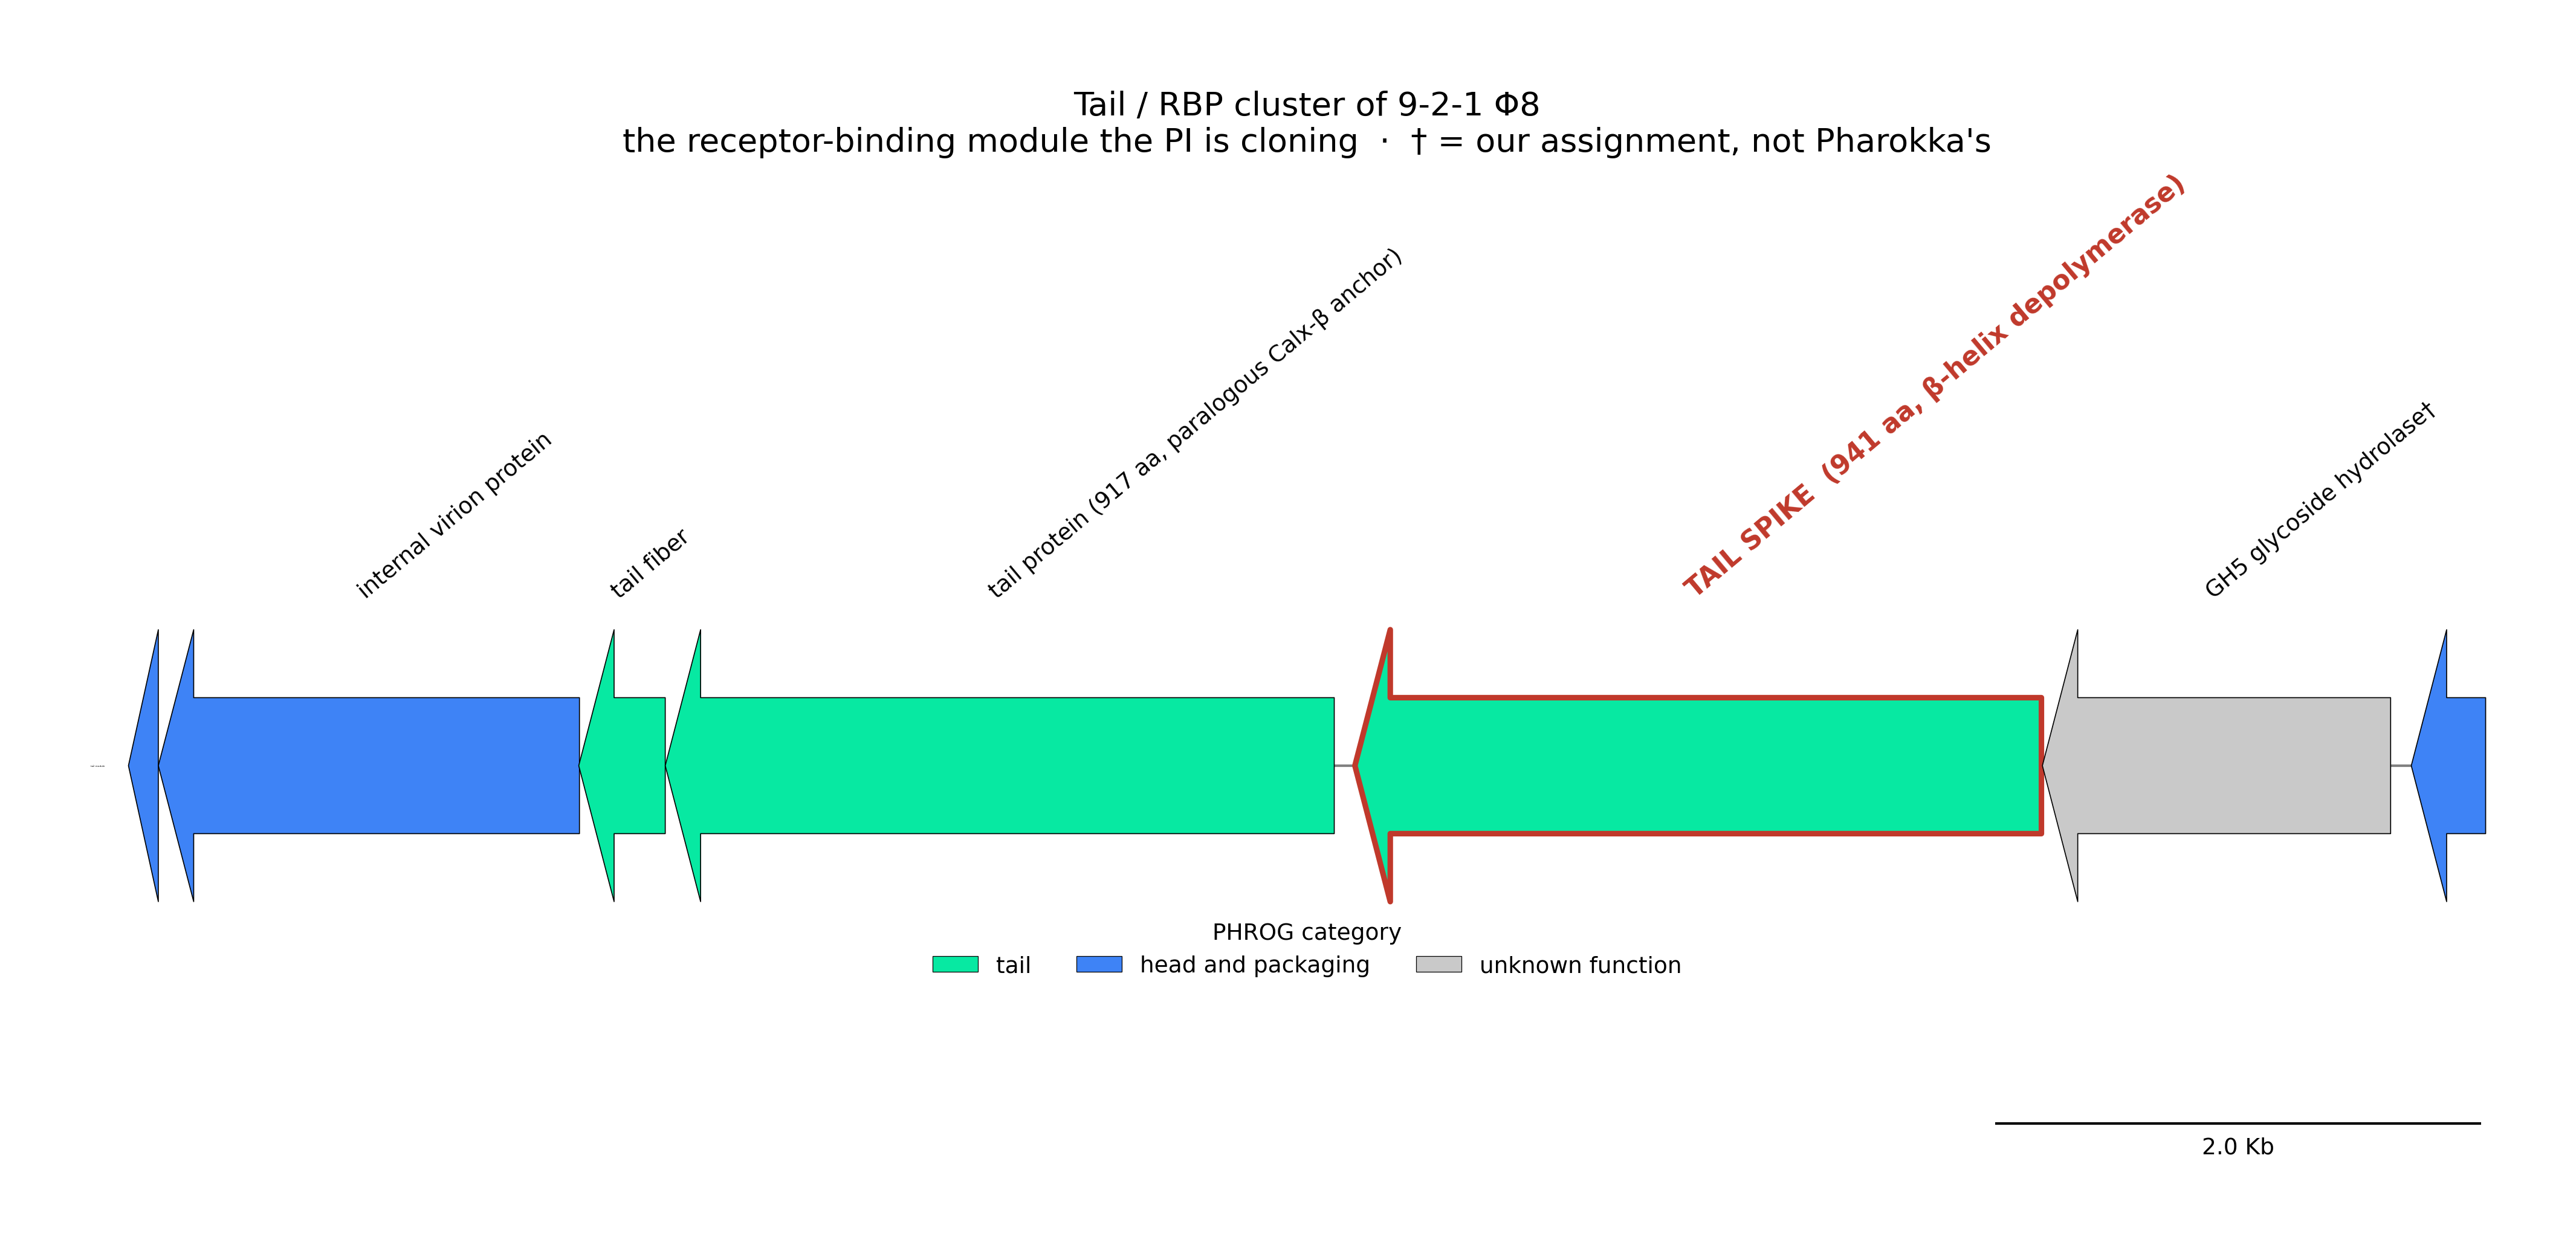
\includegraphics[width=0.98\textwidth,height=0.70\textheight,keepaspectratio]{../../code/output/0729_prof_figures/fig_phage_tail_module.png}\\
  {\scriptsize\color{muted} Numbering is the PI's \texttt{UUAIURNK\_}. The old 0708 genome map is
   mirrored — do not reuse it.}
\end{frame}

\begin{frame}{Backup 7 — enzymatic domains in full (incl.\ CDS\_0012 GH5)}
  \centering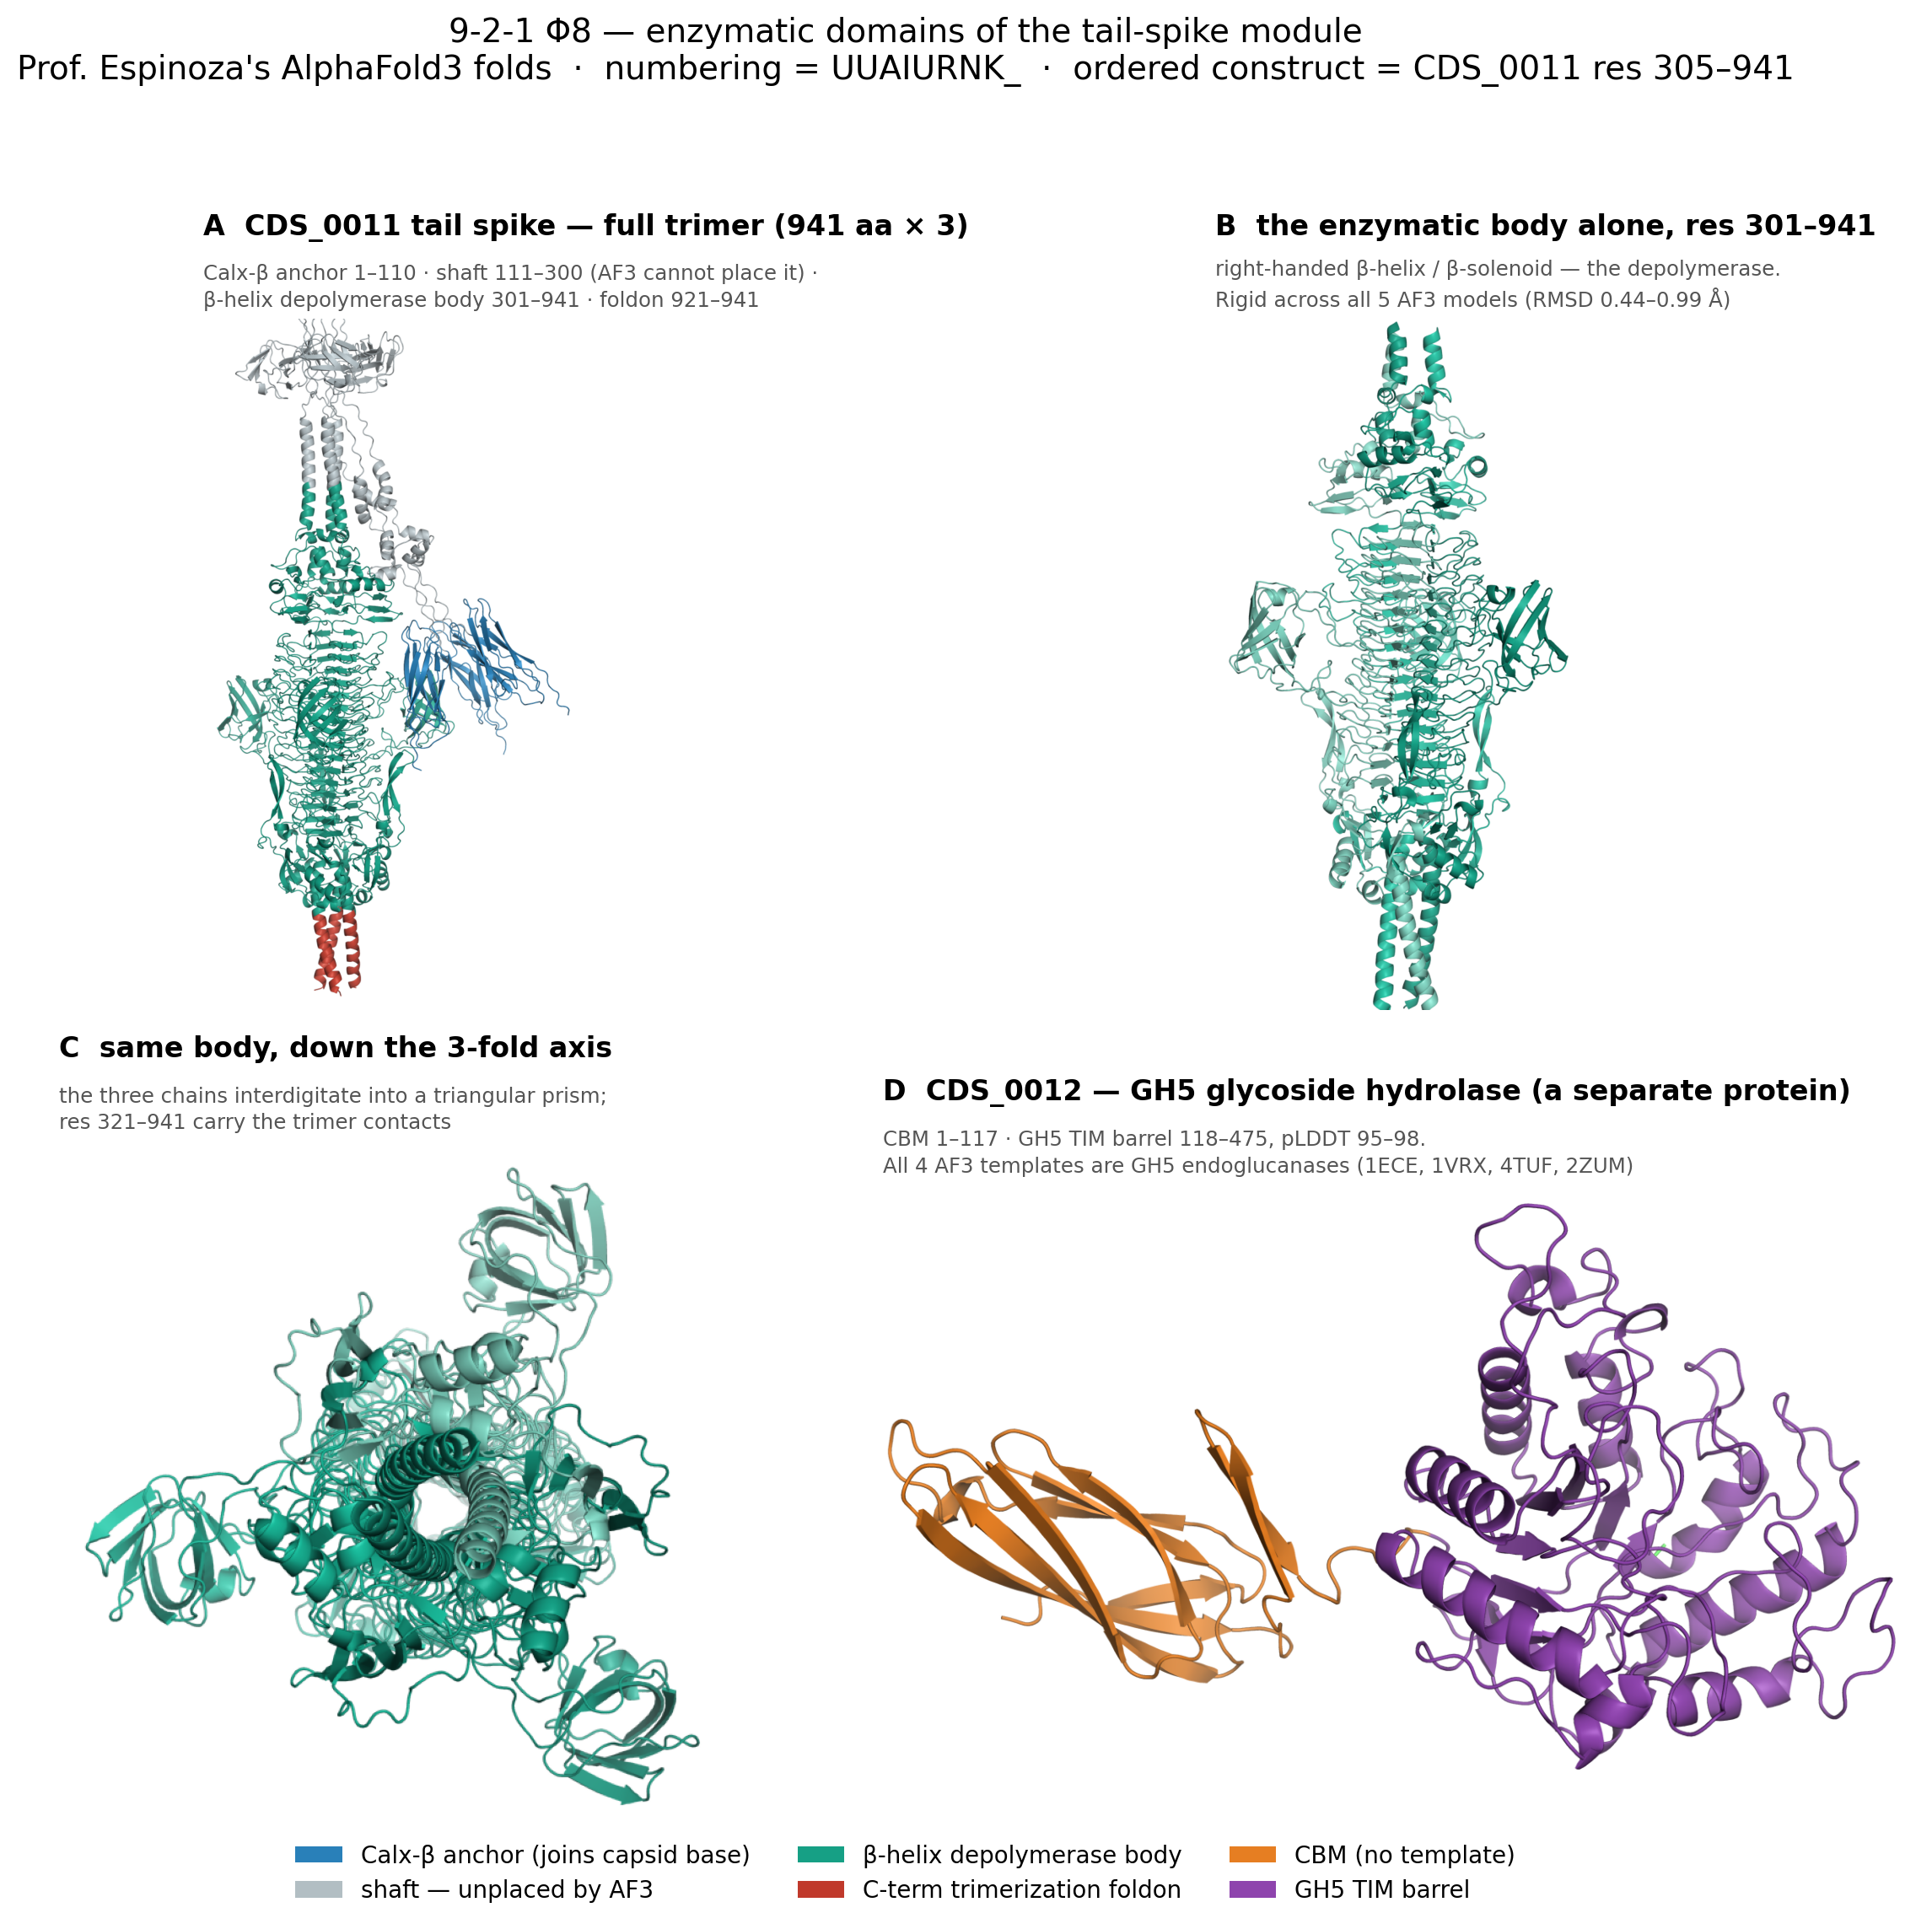
\includegraphics[width=0.68\textwidth,height=0.76\textheight,keepaspectratio]{../../code/output/0729_prof_figures/fig_enzymatic_domains.png}\\
  {\scriptsize\color{muted} Panel D is CDS\_0012 — a \textbf{separate protein}, not a domain of the
   tail spike.}
\end{frame}

\end{document}
"` prints the speaker script instead of the slides
\ifdefined\NOTESONLY \setbeameroption{show only notes}\setbeamerfont{note page}{size=\footnotesize} \fi

\begin{document}

% ---------------------------------------------------------------- 1. title
\begin{frame}[plain]
  \vspace{6pt}
  \begin{center}
    {\LARGE\bfseries Engineering the part that picks the host}\\[4pt]
    {\large Which gene, what it binds, where evolution comes in}
  \end{center}
  \vspace{4pt}
  \begin{center}
    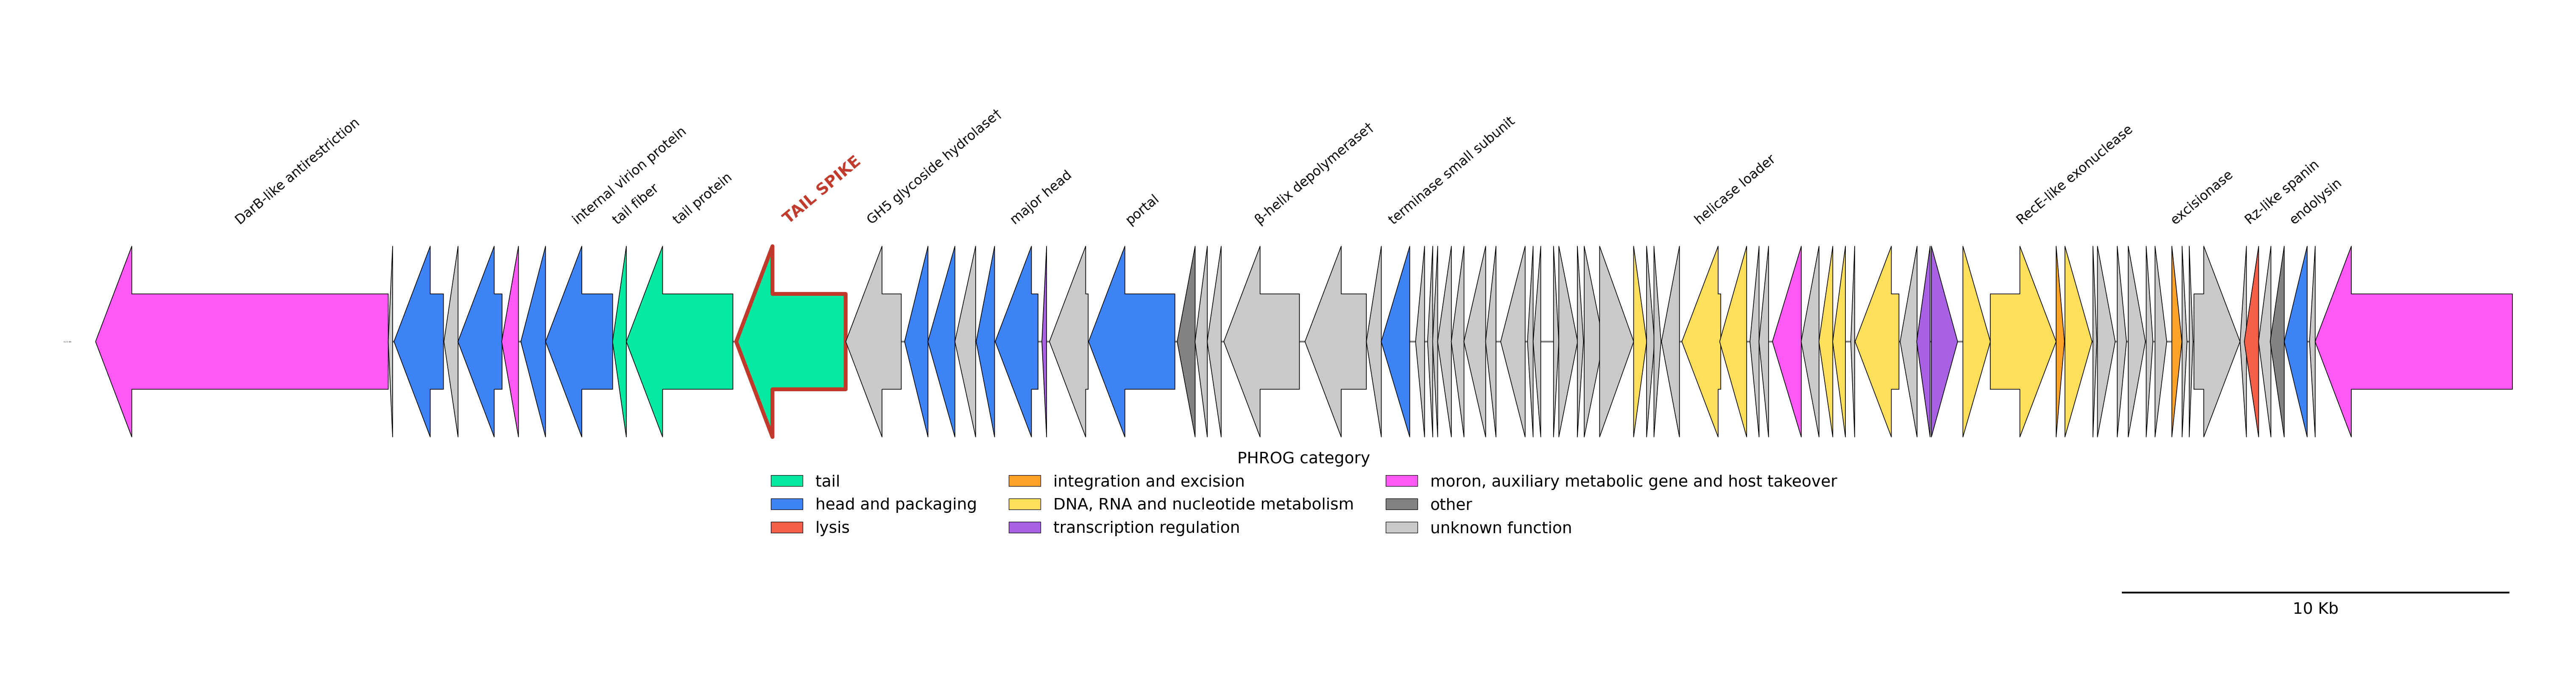
\includegraphics[width=0.95\textwidth]{fig/phage_map_banner.png}
  \end{center}
  \vspace{2pt}
  \begin{center}
  {\scriptsize\color{muted} Phage 9-2-1 $\Phi$8 — 62 kb, 80 genes — and three self-isolated
   \textit{Pseudomonas} strains\par
   \vspace{3pt}
   Chun-Yu (Alex) Chen \quad|\quad Phagenomics, Claremont CA \quad|\quad
   PI: J. Cesar Ignacio-Espinoza \quad|\quad 2026-08-21}
  \end{center}
  \note{
  Good evening. We are trying to build phage parts on purpose — to take the protein that decides which
  bacterium a phage can infect, and redesign it. Tonight: the two things you need before you can.\par
  ($\approx$18 s)}
\end{frame}

% ---------------------------------------------------------------- 2. context / goal
\begin{frame}[shrink=5]{We want to design the part, not just describe the phage}
  \begin{columns}[T,onlytextwidth]
    \begin{column}{0.53\textwidth}
      \footnotesize
      \begin{itemize}\setlength\itemsep{5pt}
        \item Phages hunt bacteria, and one phage usually infects \textbf{one strain} and ignores the
              next one over. Matching is done by \textbf{trial and error} today.
        \item Why now: \textcolor{cwzz}{\textbf{[AMR figure + source — Alex]}}. A phage is only useful
              if it hits the strain that is actually making someone sick.
        \item Our goal is a \textbf{part you can re-aim}: rebuild the receptor-binding protein so the
              same phage attacks a different strain.
        \item \textbf{We work on our own material} — local soil and water $\rightarrow$
              \textit{Pseudomonas} hosts and their phages, sequenced in house.
      \end{itemize}
      \vspace{4pt}
      \colorbox{accent!10}{\parbox{0.95\textwidth}{\centering\footnotesize
      \textbf{Tonight:} 5 isolates $\rightarrow$ \textbf{3 strains}, and one complete phage genome}}
    \end{column}
    \begin{column}{0.45\textwidth}
      \centering
      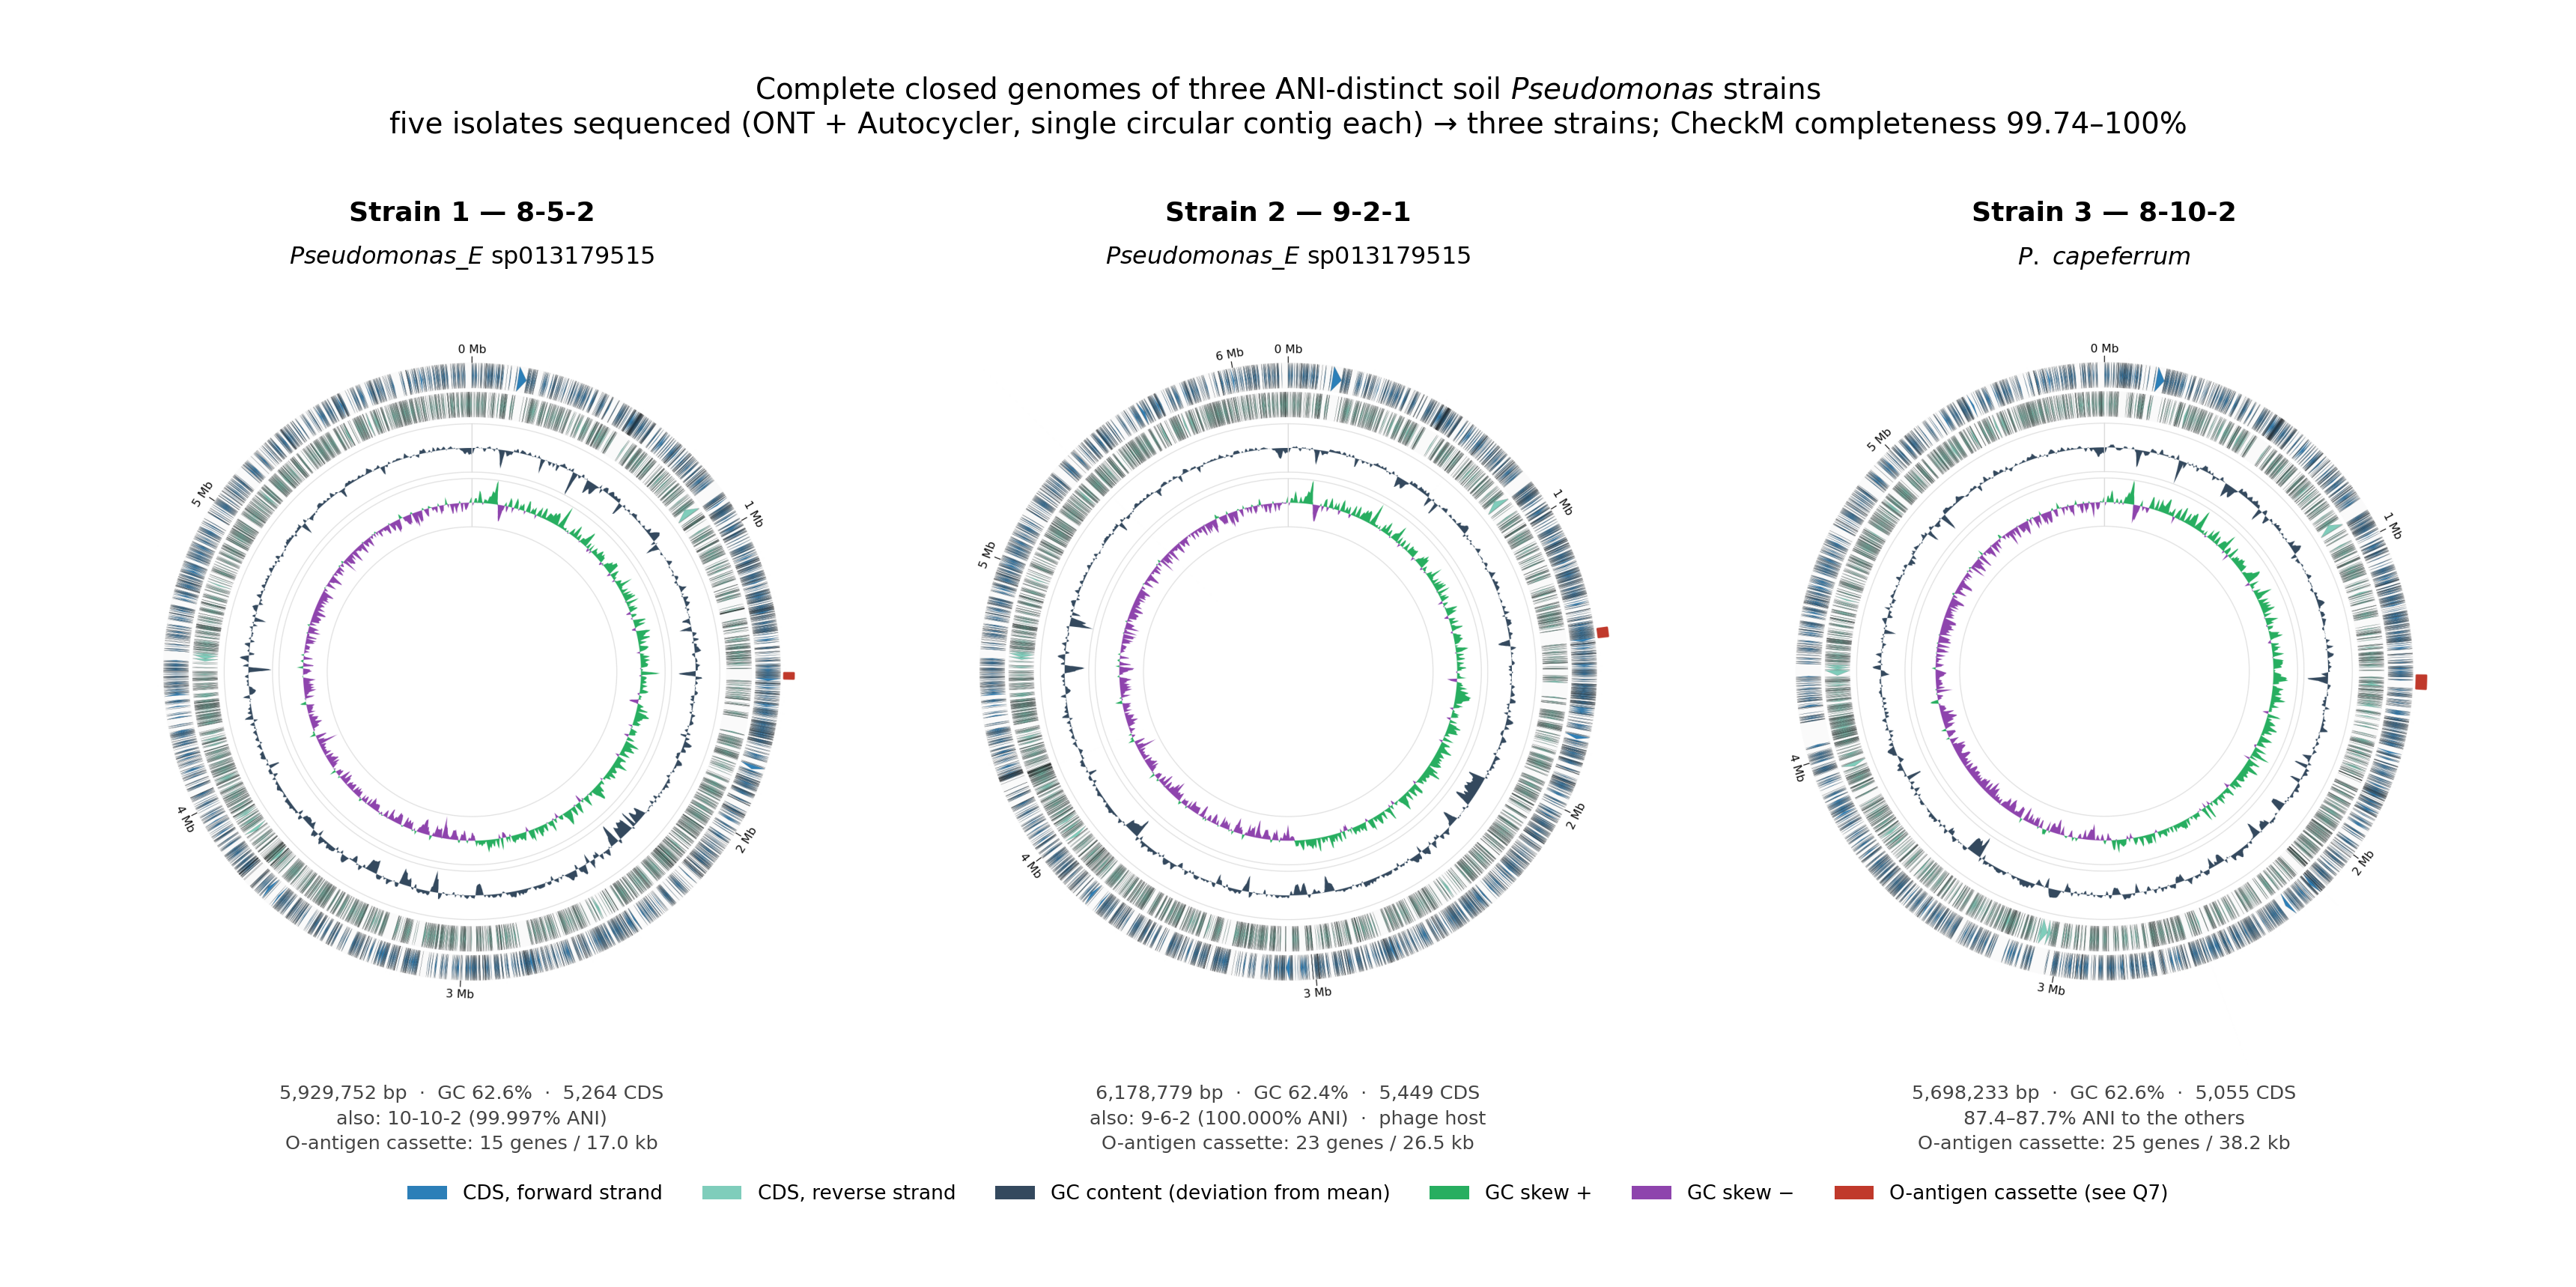
\includegraphics[width=0.98\textwidth]{../../code/output/0729_prof_figures/fig_bacterial_genomes.png}\\
      {\scriptsize\color{muted} three closed host genomes, 5.7–6.2 Mb}\\[5pt]
      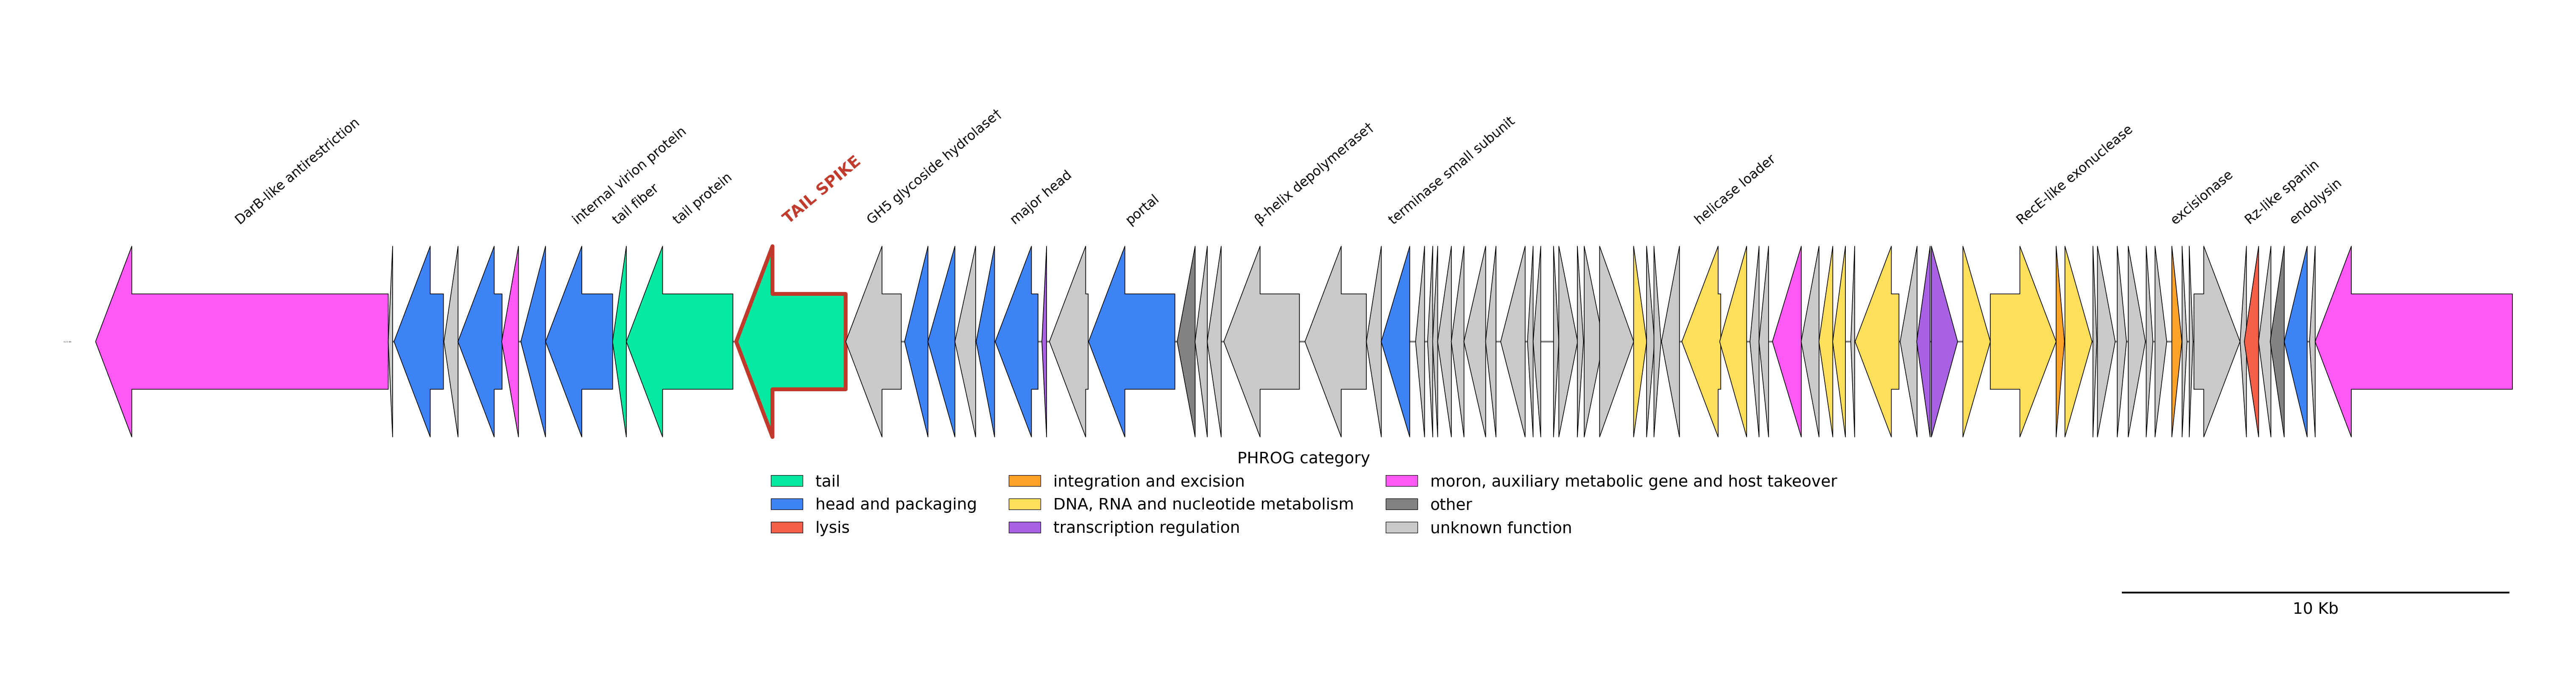
\includegraphics[width=0.98\textwidth]{fig/phage_map_banner.png}\\
      {\scriptsize\color{muted} the phage: 62 kb, 80 CDS, linear + 77 bp DTR}
    \end{column}
  \end{columns}
  \note{
  Phages hunt bacteria, and they are picky: one phage infects one strain and ignores the next one
  over. Today that match is trial and error.\par
  That matters right now — [AMR number, Alex fills in]. A phage is only useful if it hits the strain
  making someone sick.\par
  So our goal is not to describe a phage; it is to build a part you can re-aim — rebuild the
  receptor-binding protein so the same phage attacks a different strain.\par
  We work on our own material: local soil and water, Pseudomonas hosts and their phages, sequenced in
  house — five isolates, three strains, one complete phage genome.\par
  ($\approx$48 s)}
\end{frame}

% ---------------------------------------------------------------- 3. the design pipeline
\begin{frame}{The design loop — and where we actually are}
  \vspace{-2pt}
  \rqbox{Before you can redesign the targeting part: \textbf{which gene is it}, and \textbf{what must it recognise}?}
  \vspace{-2pt}
  \begin{center}
  \begin{tikzpicture}[
    font=\scriptsize,
    done/.style={draw=accent,line width=1.0pt,rounded corners=2pt,fill=accent!8,
                 text width=2.35cm,align=center,minimum height=1.8cm,inner sep=3pt},
    plan/.style={draw=muted,line width=0.9pt,dashed,rounded corners=2pt,fill=white,
                 text width=2.35cm,align=center,minimum height=1.8cm,inner sep=3pt},
    ar/.style={-{Stealth[length=4pt]},draw=muted,line width=0.7pt}]
    \node[done] (a) {\textbf{1. pick the gene}\\80 CDS $\rightarrow$ tail\\module: CDS\_0011,\\0012, 0024};
    \node[done,right=0.30cm of a] (b) {\textbf{2. define the\\target}\\fold it: what does\\it bind?};
    \node[plan,right=0.30cm of b] (c) {\textbf{3. learn from\\evolution}\\GH5 tree $\rightarrow$\\ancestral enzymes};
    \node[plan,right=0.30cm of c] (d) {\textbf{4. build\\variants}\\3 at Twist\\+ ancestral GH5};
    \node[plan,right=0.30cm of d] (e) {\textbf{5. test}\\fiber + depolymerase\\\emph{in trans}, 3 strains};
    \draw[ar] (a)--(b); \draw[ar] (b)--(c); \draw[ar] (c)--(d); \draw[ar] (d)--(e);
    \draw[ar,draw=muted,dashed] (e.south) -- ++(0,-0.35) -| node[pos=0.25,below,font=\scriptsize\color{muted}]{design rules} (c.south);
  \end{tikzpicture}
  \end{center}
  \vspace{2pt}
  {\scriptsize\color{muted} \tikz[baseline=-0.5ex]\draw[accent,line width=1pt,fill=accent!8] (0,0) rectangle (1.6ex,1.6ex);
   solid = has data \quad
   \tikz[baseline=-0.5ex]\draw[muted,dashed,line width=0.9pt] (0,0) rectangle (1.6ex,1.6ex);
   dashed = in progress / proposed \quad|\quad the next two slides are steps 1 and 2}
  \note{
  Here is the loop. Step one, pick the gene: of 80 genes the structural module narrows it to a
  handful — the tail spike, the GH5 beside it, and a depolymerase the annotator missed.\par
  Step two, define the target — you cannot redesign a binder without knowing what it binds.\par
  Step three is where evolution comes in. The tail spike decides who is recognised; the depolymerase
  decides what can be cut open. So we build a tree over all GH5 sequences and reconstruct ancestral
  enzymes — proteins from different points in evolution, not random mutants. Stated caveat: this
  assumes affinity tracks infection.\par
  Step four, build them: three constructs are at Twist, ancestral enzymes next. Step five, combine
  fiber and depolymerase in trans on our three strains, and feed that back as design rules.\par
  Solid boxes have data; dashed ones do not. The next two slides are steps one and two.\par
  ($\approx$62 s)}
\end{frame}

% ---------------------------------------------------------------- 4. result 1 — the part
\begin{frame}[shrink=5]{Steps 1--2: a $\beta$-helix depolymerase — the target is a sugar}
  \begin{columns}[T,onlytextwidth]
    \begin{column}{0.30\textwidth}
      \centering
      \includegraphics[height=0.60\textheight]{../../code/output/0729_prof_figures/panels/cds0011_trimer_domains.png}\\[2pt]
      {\scriptsize\color{muted} CDS\_0011 trimer, 941 aa $\times$ 3\par
       grey shaft \textbullet\ blue anchor\par
       \textcolor{accent}{\textbf{teal body}} \textbullet\ red foldon}
    \end{column}
    \begin{column}{0.68\textwidth}
      \footnotesize
      \begin{itemize}\setlength\itemsep{5pt}
        \item Right-handed \textbf{$\beta$-helix}, one rung every \textbf{15–18 residues} — the
              signature of a polysaccharide depolymerase. \textbf{This part cuts sugar}, so its target
              is the surface sugar, not a protein.
        \item The domain map is what makes it \textbf{engineerable}: pLDDT 88–94, and the body
              (res 301–941) is rigid to \textbf{0.44–0.99 \AA} across five models — that boundary is
              exactly where our construct starts (res 305).
        \item The protein--protein hypothesis was tested first \textbf{and failed}:
      \end{itemize}
      \vspace{1pt}
      \begin{center}
        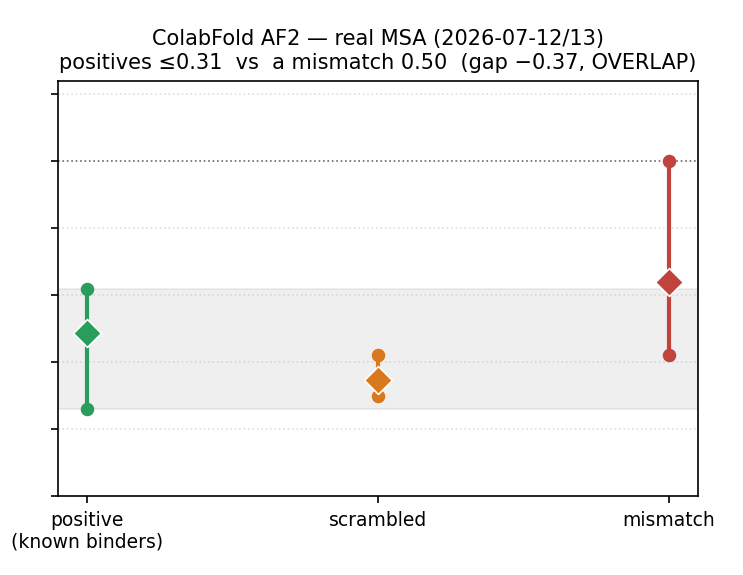
\includegraphics[height=0.25\textheight]{fig/binding_controls_af2.png}\\
        {\scriptsize\color{muted} positives ipTM $\leq$ 0.31 vs a mismatched pair 0.50 — no signal}
      \end{center}
    \end{column}
  \end{columns}
  \note{
  Steps one and two on one slide. This is the tail spike, 941 residues, a trimer: grey shaft AlphaFold
  cannot place, blue anchor into the capsid, teal working body.\par
  That body is a right-handed beta helix, one rung every 15 to 18 residues — the signature of a
  depolymerase. So the part cuts sugar, and its target is the surface sugar, not a protein.\par
  It is also engineerable: the body from residue 301 is rigid, under one angstrom across five models,
  and that boundary is exactly where our construct starts.\par
  And we tested the protein-protein hypothesis first — docking gave positives at 0.31 and a mismatch
  at 0.50. No discriminating power, so we retired that screen.\par
  ($\approx$57 s)}
\end{frame}

% ---------------------------------------------------------------- 5. result 2 — the target varies
\begin{frame}[shrink=5]{The target is different in every strain — that is the handle}
  \vspace{1pt}
  \footnotesize Same \texttt{ihfB}-flanked slot, different cargo
   \ \textcolor{muted}{(grey ribbons = homology)}\normalsize
  \vspace{1pt}
  \begin{center}
    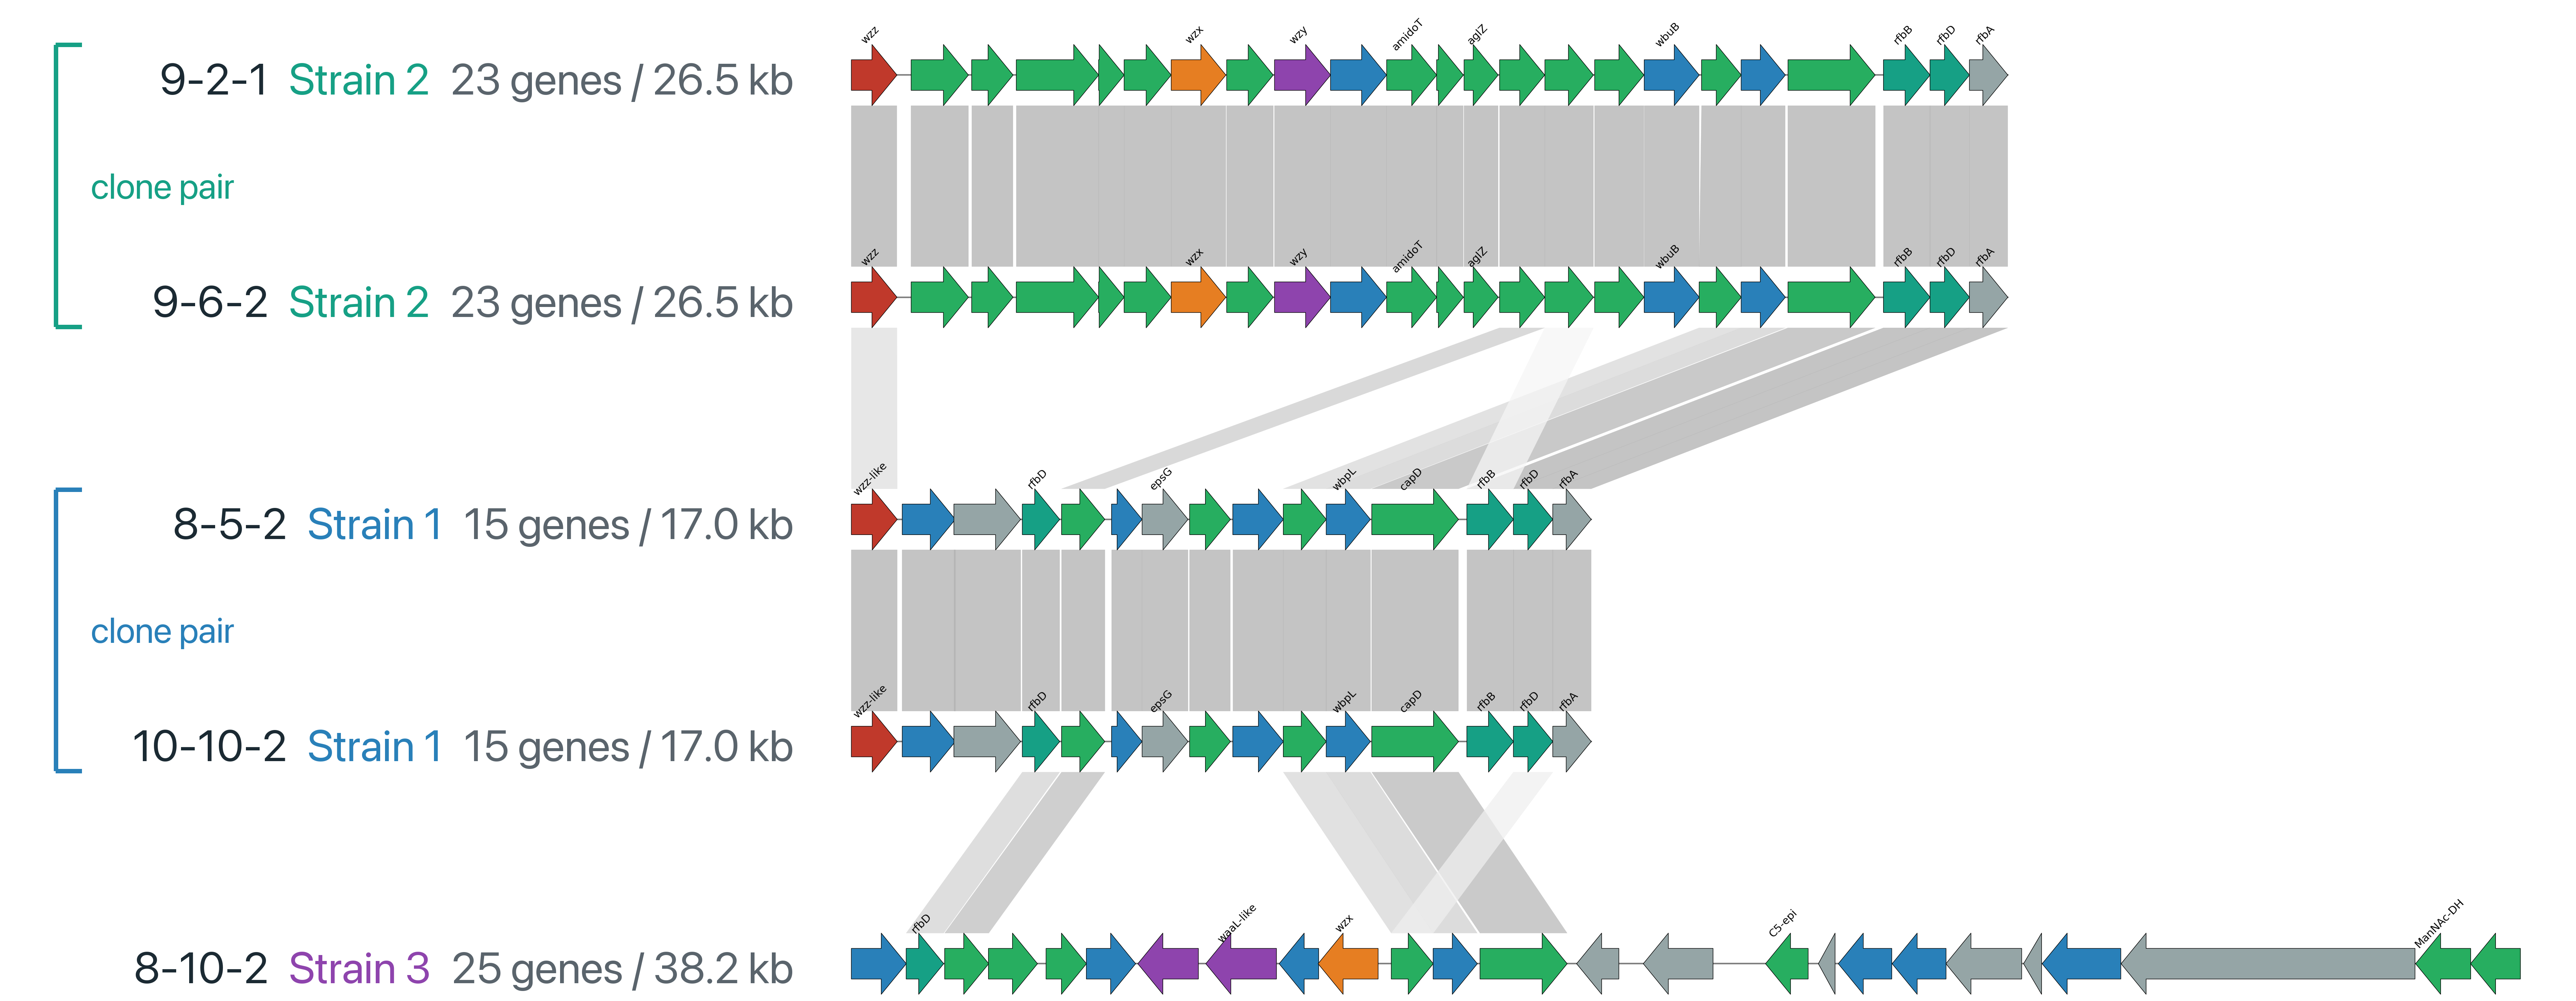
\includegraphics[width=0.95\textwidth,height=0.54\textheight,keepaspectratio]{fig/oantigen_tracks_labeled.png}
  \end{center}
  \vspace{-4pt}
  \begin{center}\tiny
    \chip{cwzz}{chain-length regulator}\quad\chip{cwzx}{flippase (wzx)}\quad\chip{cwzy}{polymerase (wzy)}\quad
    \chip{cgt}{glycosyltransferase}\quad\chip{crha}{dTDP-rhamnose}\quad\chip{cnuc}{nucleotide-sugar}\quad
    \chip{cother}{unassigned}
  \end{center}
  \vspace{1pt}
  {\footnotesize \textbf{4 of 45 clusters shared by all three} — generic sugar chemistry only, no
   shared assembly machinery. \textcolor{muted}{Control: clone pairs 100.0\% identical.}}
  \note{
  If the part reads a sugar, does that sugar differ between strains? That difference is the handle a
  redesigned part would turn.\par
  Five tracks: two Strain 2 clones, two Strain 1 clones, Strain 3; arrows are genes, grey ribbons are
  homology. Control first: inside each clone pair all 23 and all 15 genes are identical. ANI
  saturates, so this had to be measured.\par
  Across strains the links are sparse and crossed — of 45 clusters only four are shared, all generic
  sugar chemistry, no shared flippase, polymerase or chain-length regulator.\par
  Three strains, three targets. This phage should not plaque on the other two, and a re-aimed part is
  what would change that.\par
  ($\approx$57 s)}
\end{frame}

% ---------------------------------------------------------------- 6. close
\begin{frame}[shrink=5]{Where the loop stands}
  \begin{columns}[T,onlytextwidth]
    \begin{column}{0.50\textwidth}
      \small
      \textcolor{accent}{\textbf{Conclusion}}\\
      We know \textbf{which gene} to engineer and \textbf{what it must recognise}: the tail-spike
      depolymerase, against a strain-specific O-antigen — and our three strains give three different
      targets.
      \vspace{6pt}

      \textcolor{accent}{\textbf{Limitation}}\\
      Steps 3–5 are \textbf{not results yet}: the GH5 ancestral reconstruction is still being built,
      the constructs are not expressed, and the cross-strain plaque assay was run July 4 but the data
      is not in our hands. It also assumes affinity tracks infection. No serotyping tool exists for
      this taxon, so we cannot name an O-type.
      \vspace{6pt}

      \textcolor{accent}{\textbf{Next three months}}\\
      Recover that readout; express the three constructs; reconstruct ancestral GH5 enzymes and test
      fiber $+$ depolymerase \emph{in trans} on the three strains. The tail spike also has a
      15,775-sequence alignment — enough for a conservation profile on the structure.
    \end{column}
    \begin{column}{0.48\textwidth}
      \centering
      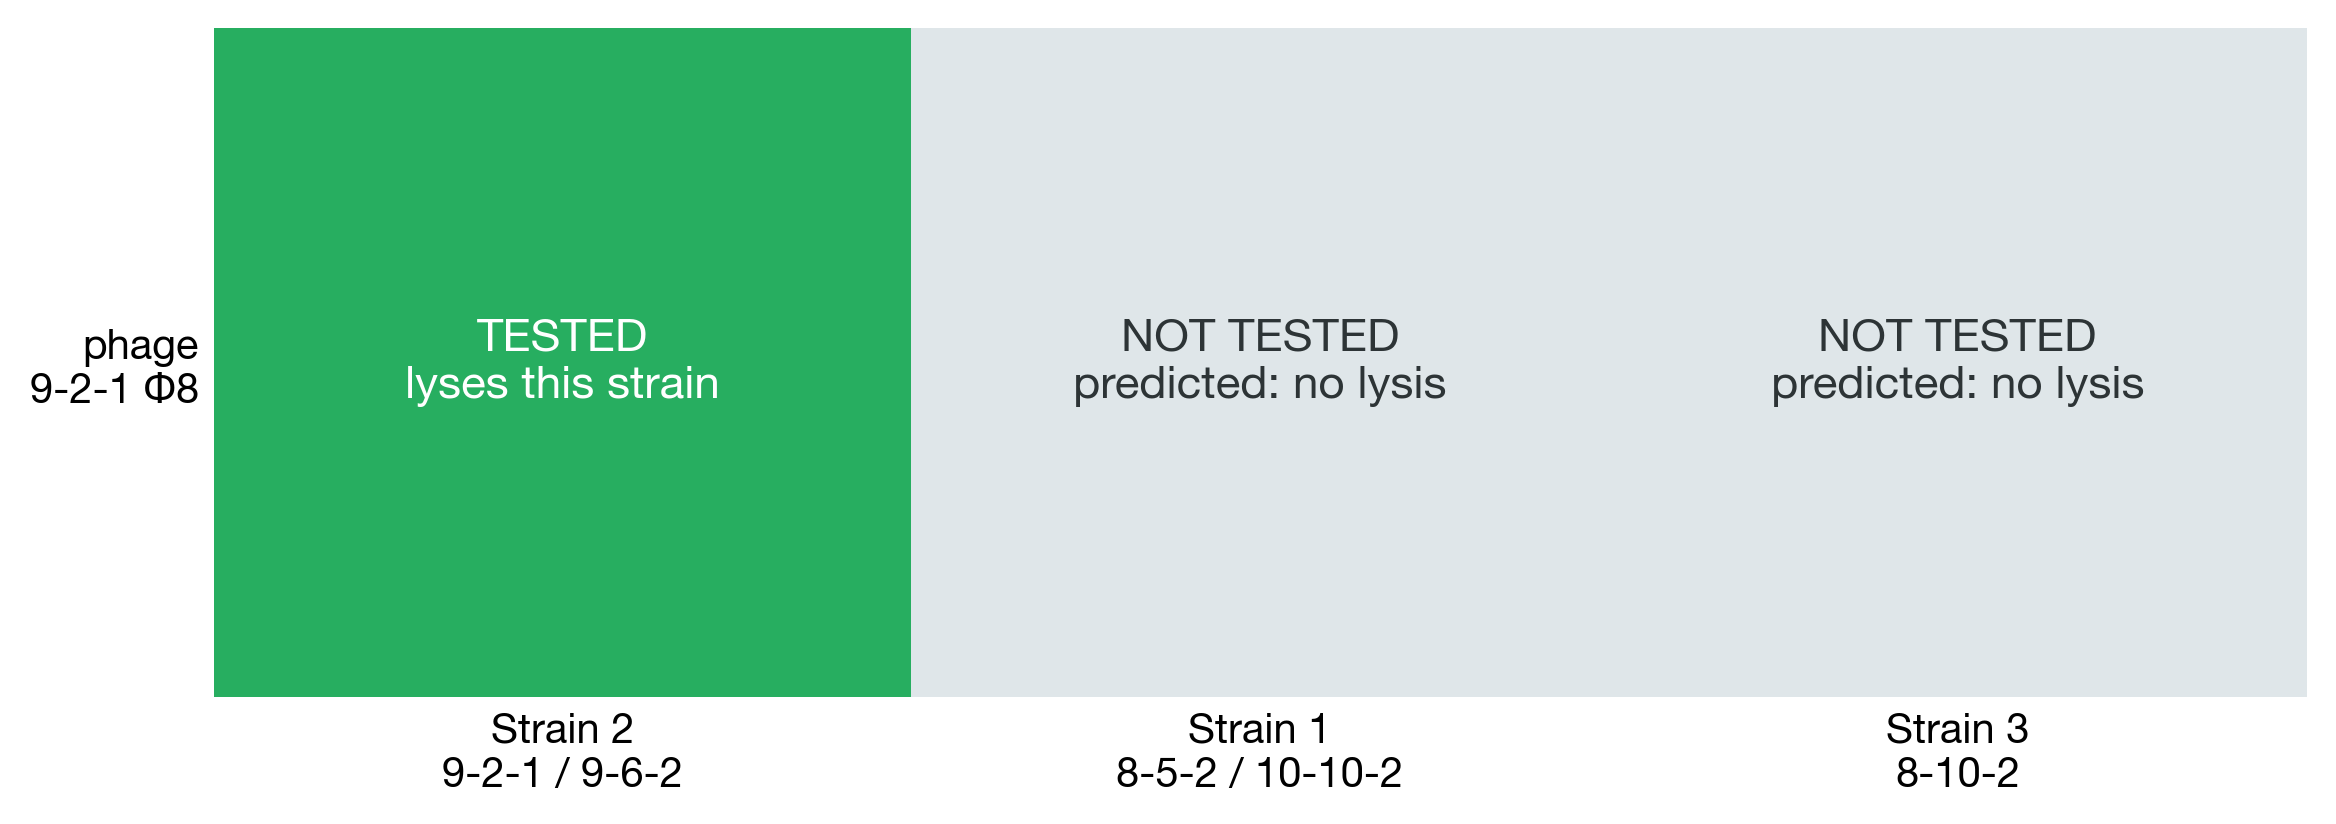
\includegraphics[width=\textwidth]{fig/hostrange_cells.png}\\[3pt]
      {\scriptsize\color{muted} only Strain 2 has actually been challenged; the grey cells are
       predictions, and the July 4 assay reads them out}\\[8pt]
      \begin{flushleft}\scriptsize
      \textcolor{accent}{\textbf{1. pick the gene}} — done\\
      \textcolor{accent}{\textbf{2. define the target}} — done\\
      \textcolor{muted}{\textbf{3. ancestral GH5 enzymes} — PI building the tree}\\
      \textcolor{muted}{\textbf{4. build} — 3 constructs at Twist}\\
      \textcolor{muted}{\textbf{5. test} — \emph{in trans}, waiting on the July 4 readout}
      \end{flushleft}
    \end{column}
  \end{columns}
  \vspace{5pt}
  \begin{center}\large\bfseries We now know which part to rebuild and what it has to grip — the
   ancestral variants are the next lever.\end{center}
  \note{
  Where the loop stands. We know which gene to engineer and what it must recognise — the tail-spike
  depolymerase against a strain-specific O-antigen — and three strains give three targets.\par
  The limitation is honest: steps three to five are not results — the GH5 tree is still being built,
  the constructs are not expressed, and the July fourth plaque data is not in our hands. And no
  serotyping tool exists for this taxon, so we cannot name an O-type.\par
  Next three months: recover that readout, express the constructs, and reconstruct ancestral GH5
  enzymes — then measure how proteins from different points in evolution behave with the fiber, in
  trans, on the three strains.\par
  We know which part to rebuild and what it has to grip. The ancestral variants are the next lever.\par
  ($\approx$58 s — stop here, not on a thank-you slide)}
\end{frame}

% ================================================================ backup
\begin{frame}[plain]
  \vspace{1.2cm}\centering{\Large\bfseries Backup}\\[4pt]{\color{muted} not shown unless asked}
\end{frame}

\begin{frame}{Backup 1 — gene selection and the constructs}
  \small
  \begin{itemize}\setlength\itemsep{5pt}
    \item Structural module, in canonical podovirus order: portal (CDS\_0020) $\rightarrow$ major
          capsid (0017) $\rightarrow$ adaptors $\rightarrow$ \textbf{tail spike (0011)} $\rightarrow$
          tail (0010) $\rightarrow$ fiber (0009).
    \item \textbf{CDS\_0024 is a second $\beta$-helix depolymerase} (rung 22–24) that Pharokka called
          ``hypothetical''; the de-novo RBP classifier found it at score 0.998.
    \item \textbf{CDS\_0012 is a GH5 glycoside hydrolase} — a separate protein, not a domain of the
          tail spike; all four AF3 templates are GH5 endoglucanases.
    \item Ordered from Twist 2026-07-27, all in pET-28a(+) with N-terminal His6:
          CDS\_0011 res \textbf{305–941} (the rigid body), CDS\_0010 res 105–917,
          CDS\_0012 res 117–477.
    \item CDS\_0010 is an \textbf{unknown protein} — the glycosidase call was withdrawn 2026-07-29;
          it is being expressed for functional characterisation.
  \end{itemize}
\end{frame}

\begin{frame}{Backup 2 — how the locus was pulled, how orthology was called}
  \small
  \begin{itemize}\setlength\itemsep{5pt}
    \item Anchor, identical in all five genomes: 30S ribosomal protein S1 $\rightarrow$ \texttt{ihfB}
          $\rightarrow$ LPS assembly protein A $\rightarrow$ MBL-fold hydrolase $\rightarrow$
          \textbf{cassette starts}. \texttt{ihfB} is the canonical upstream flank of the
          \textit{Pseudomonas} OSA cluster in the literature.
    \item Orthology = MMseqs2 clustering, $\geq$30\% identity / $\geq$50\% coverage.
          \textbf{Product names cannot be used}: the chain-length regulators of Strain 1 and Strain 2
          carry different Bakta labels but are homologous by sequence.
    \item Locus sizes: Strain 2 = 23 genes / 26.5 kb \textbullet\ Strain 1 = 15 / 17.0 kb \textbullet\
          Strain 3 = 25 / 38.2 kb.
    \item The cross-strain best-hit numbers (9/23, 10/23, 6/15) are one-directional best hits at a
          looser cutoff and are not meant to reconcile with the 45/4 cluster counts.
  \end{itemize}
\end{frame}

\begin{frame}{Backup 3 — cluster matrix, 45 clusters $\times$ 3 strains}
  \centering
  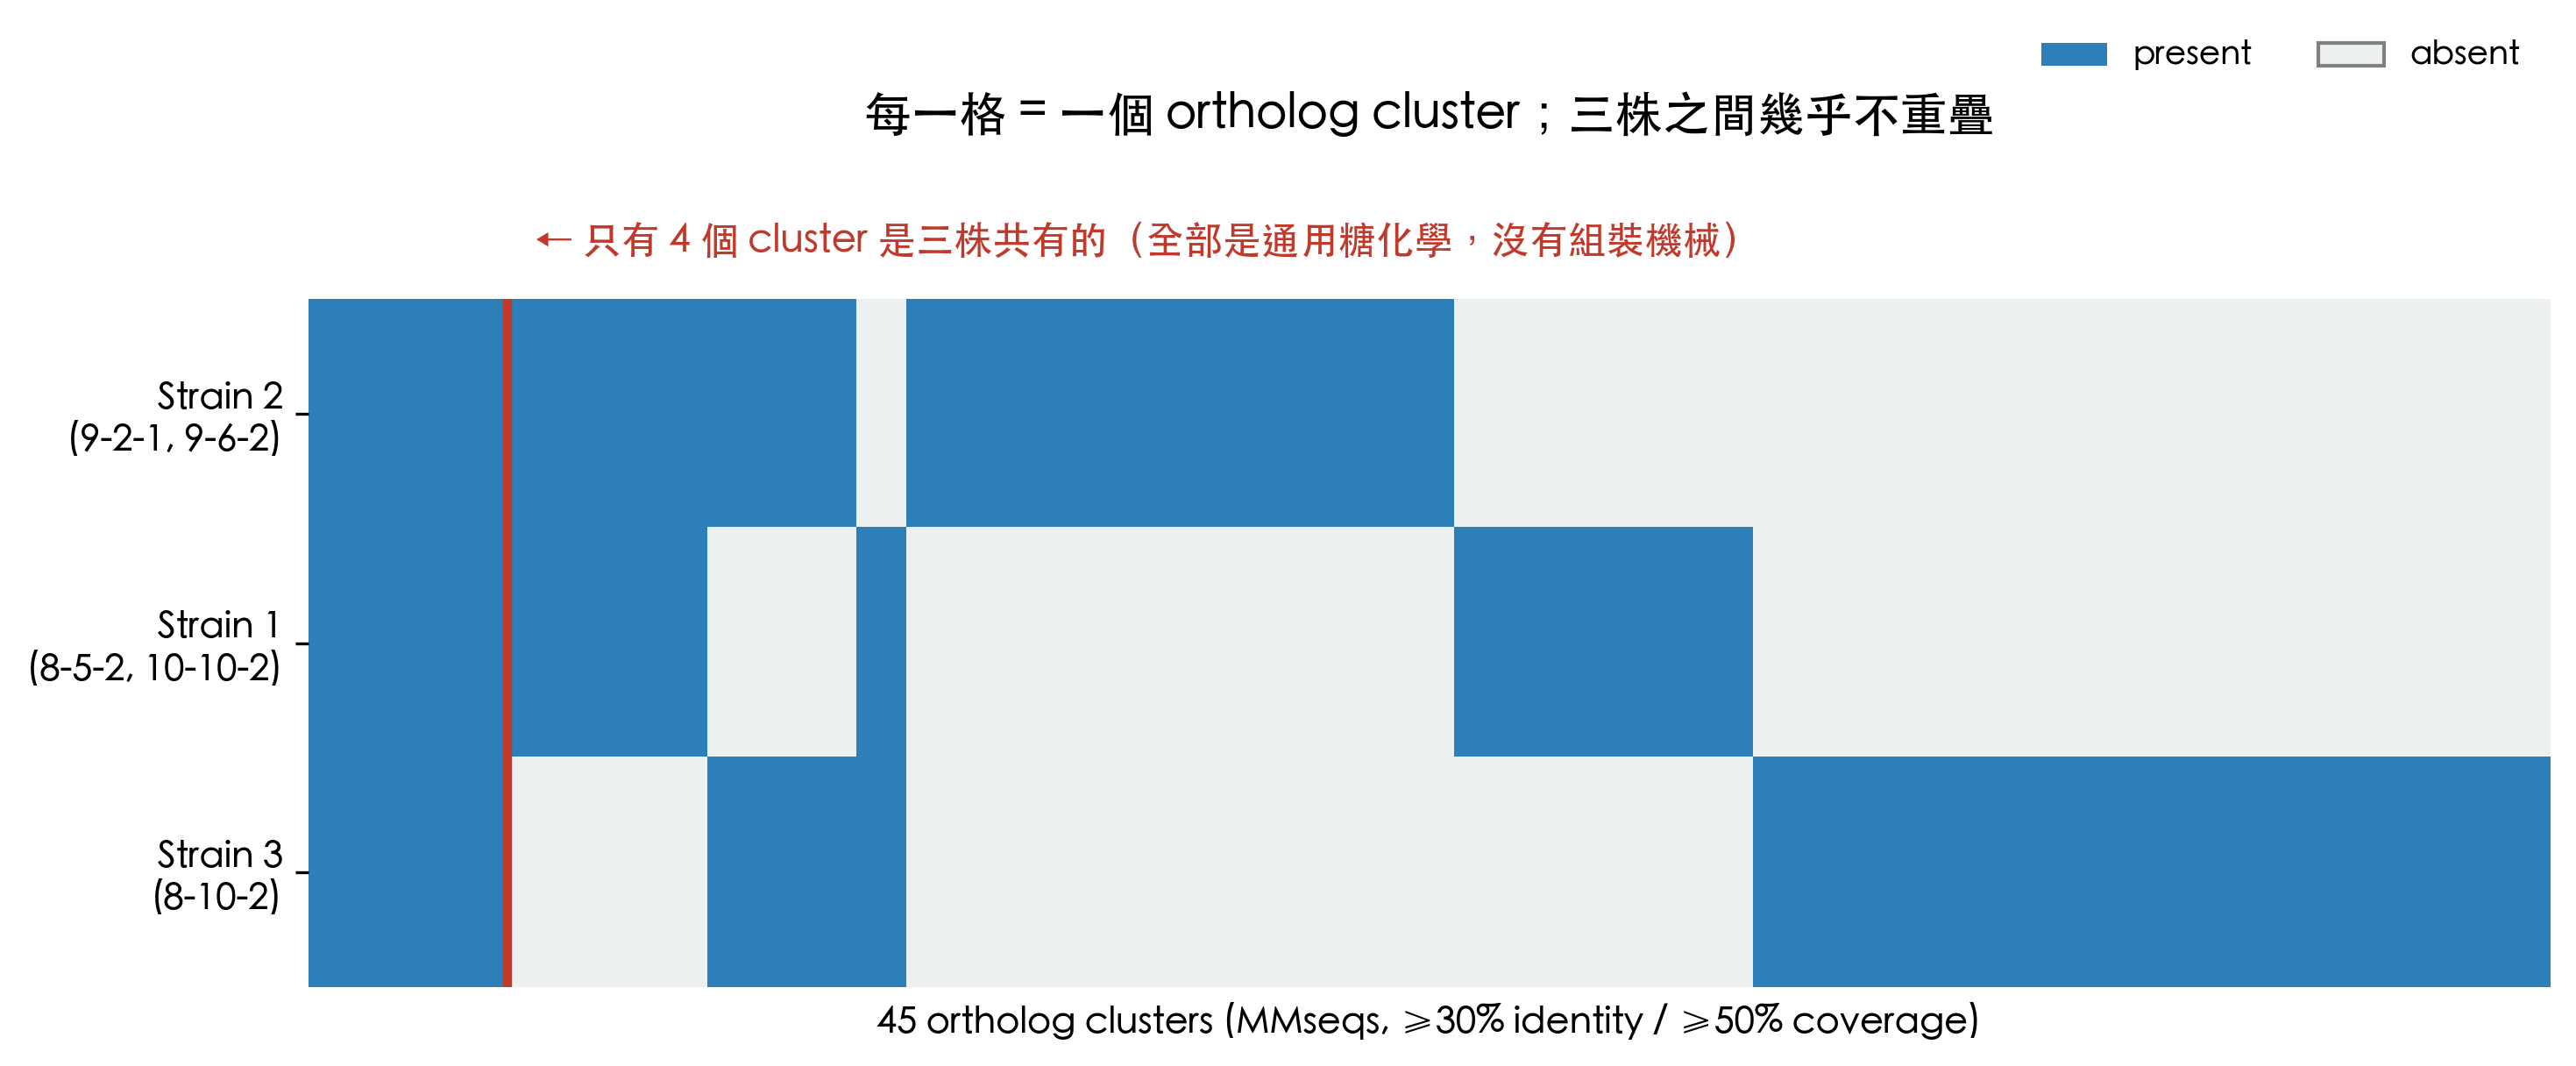
\includegraphics[width=0.86\textwidth,height=0.74\textheight,keepaspectratio]{../../code/output/0727_o_antigen_comparison/fig2_cluster_presence.png}
\end{frame}

\begin{frame}{Backup 4 — limitations in full}
  \small
  \begin{itemize}\setlength\itemsep{5pt}
    \item \textbf{Variable $\neq$ specificity-determining.} An earlier plan to read specificity off
          metagenomic variable regions was rejected in our own review: metagenome sequences carry no
          host labels, so specificity-determining positions cannot be identified that way. The
          15,775-sequence alignment (tail spike, CDS\_0011) supports a \textbf{conservation profile}
          — not ``these residues set the host range''. The ancestral reconstruction the PI is building
          is a separate thing: a tree over \textbf{all GH5 sequences} (CDS\_0012), whose ancestral
          enzymes get expressed and challenged \emph{in trans}, under the stated caveat that
          affinity $\sim$ binding $\sim$ infection.
    \item \textbf{Do not say Strain 1 lacks a flippase or polymerase} — Bakta assigns no Pfam/InterPro
          to those two genes; confirming them needs InterProScan.
    \item \textbf{The sugar structure has not been measured} — gene content is not structure; that
          needs LPS extraction and mass spectrometry.
    \item \textbf{The $\beta$-helix has no named structural homolog yet} — no foldseek or DALI run.
    \item \textbf{Taxonomy}: the virion module is podovirus-like, but reciprocal best hits against T7,
          $\varphi$KMV and KP32 are $\approx$0 and the genome carries an excisionase; \textit{terL} is
          unannotated, so formal taxonomy cannot be run. ``T7-like'' is an organizational analogy only.
  \end{itemize}
\end{frame}

\begin{frame}{Backup 5 — the three host genomes}
  \centering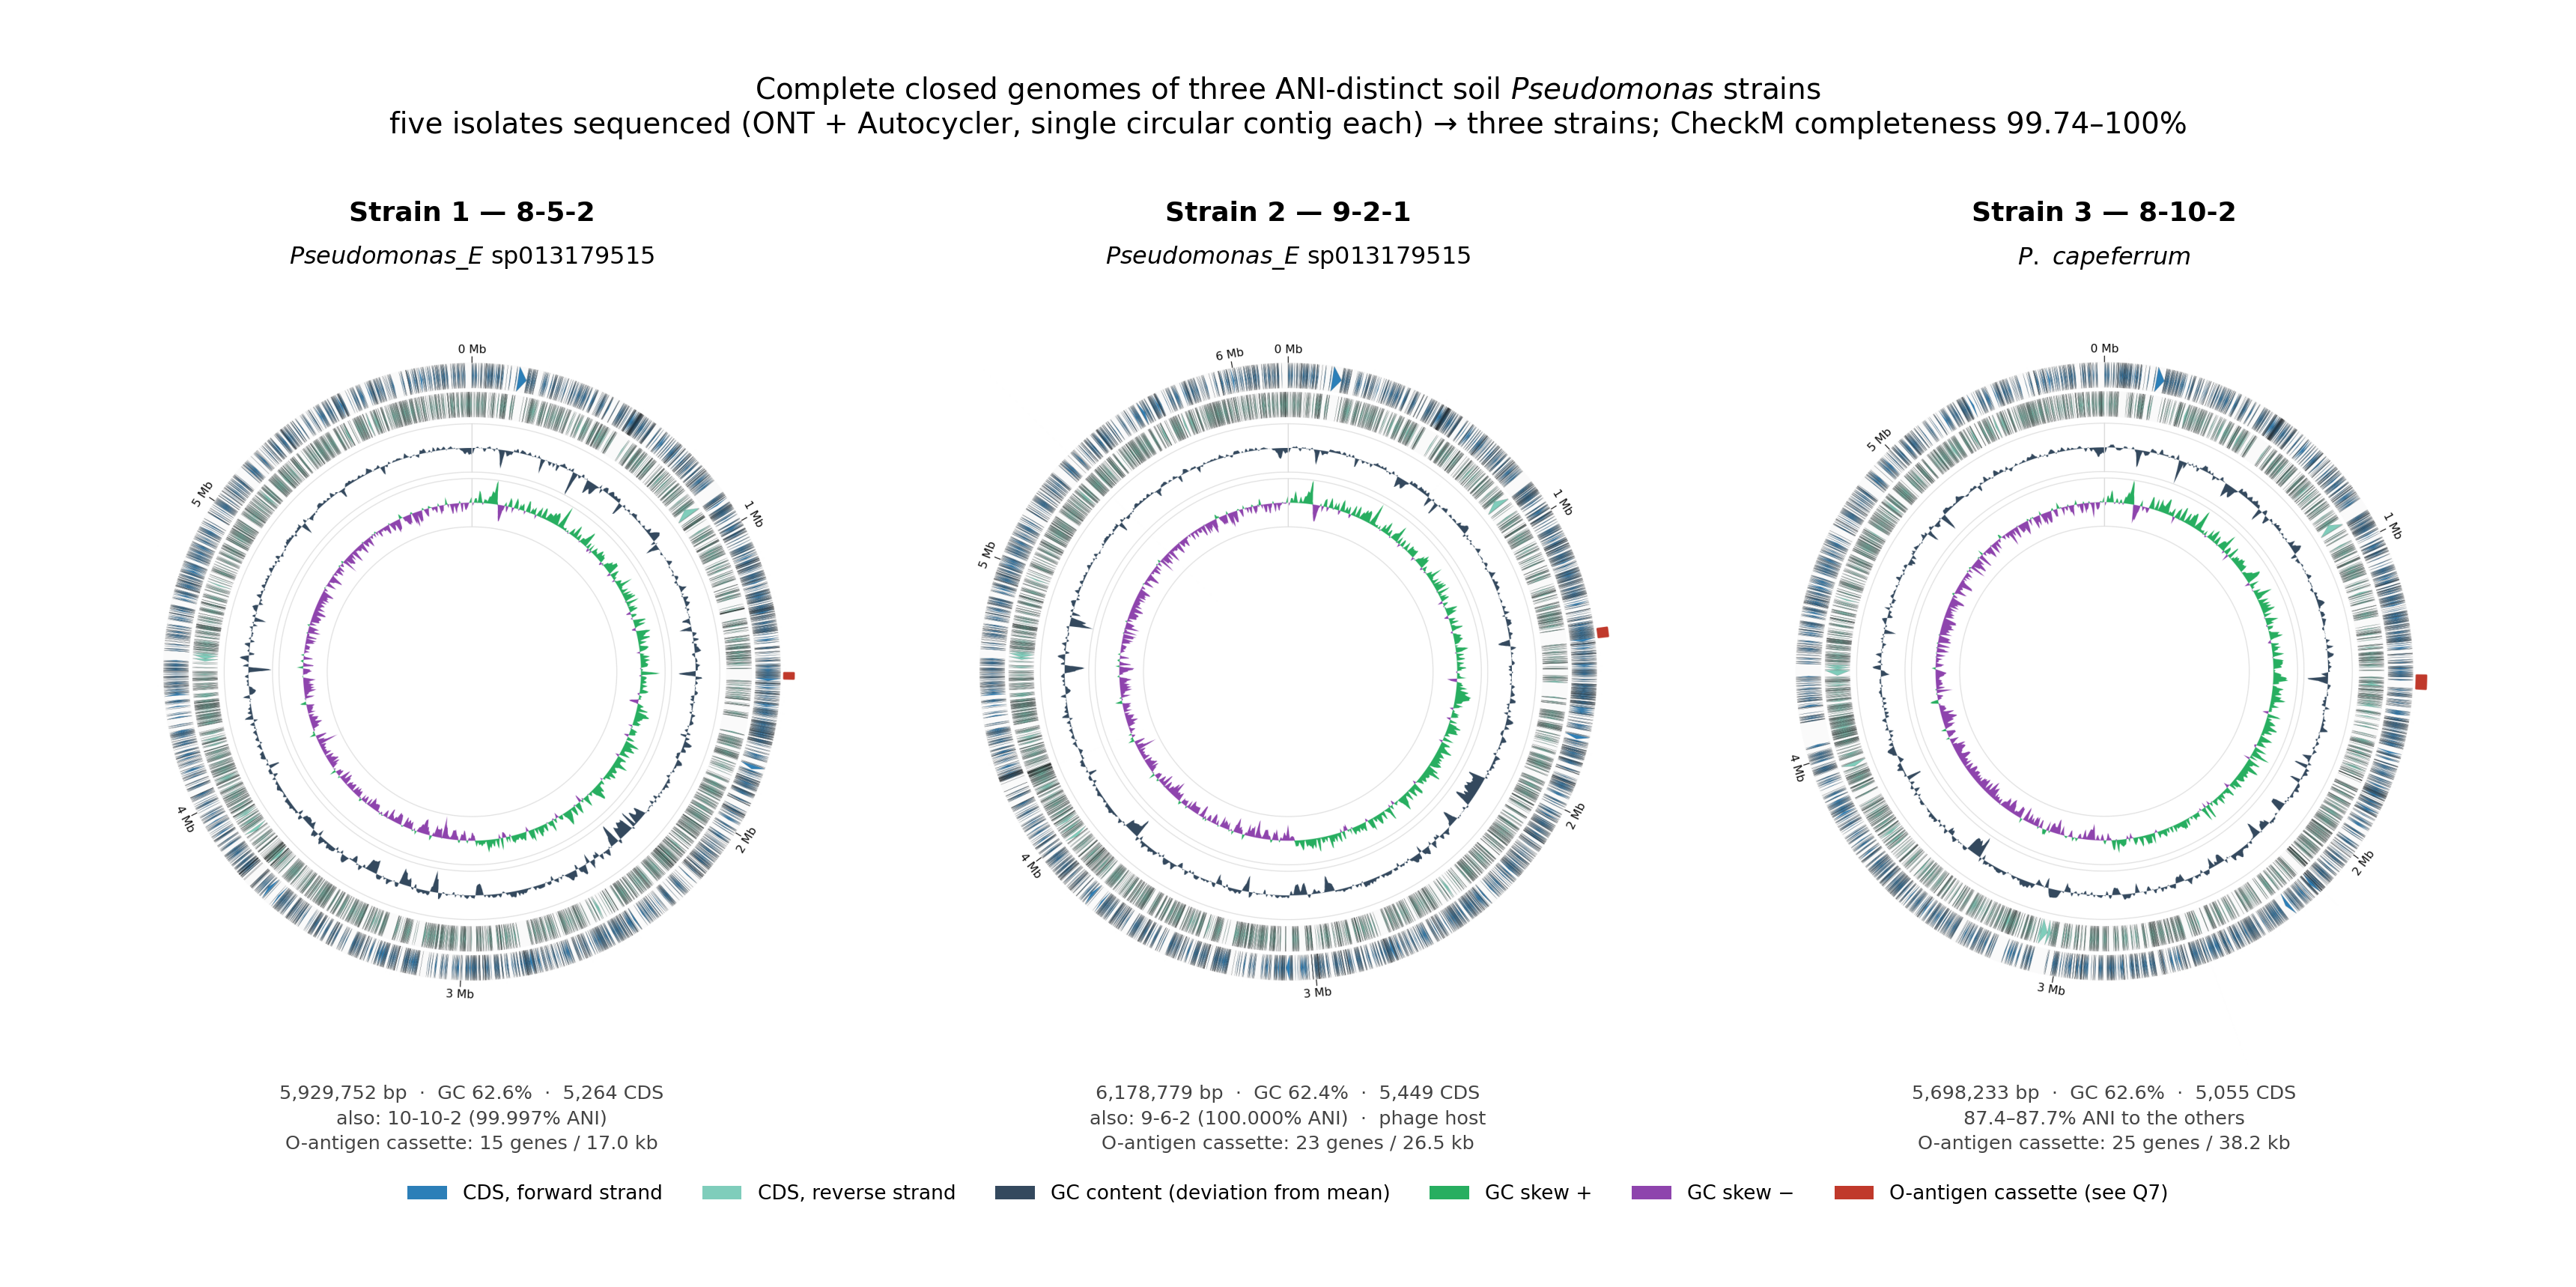
\includegraphics[width=0.95\textwidth,height=0.78\textheight,keepaspectratio]{../../code/output/0729_prof_figures/fig_bacterial_genomes.png}
\end{frame}

\begin{frame}{Backup 6 — phage genome, tail / RBP module}
  \centering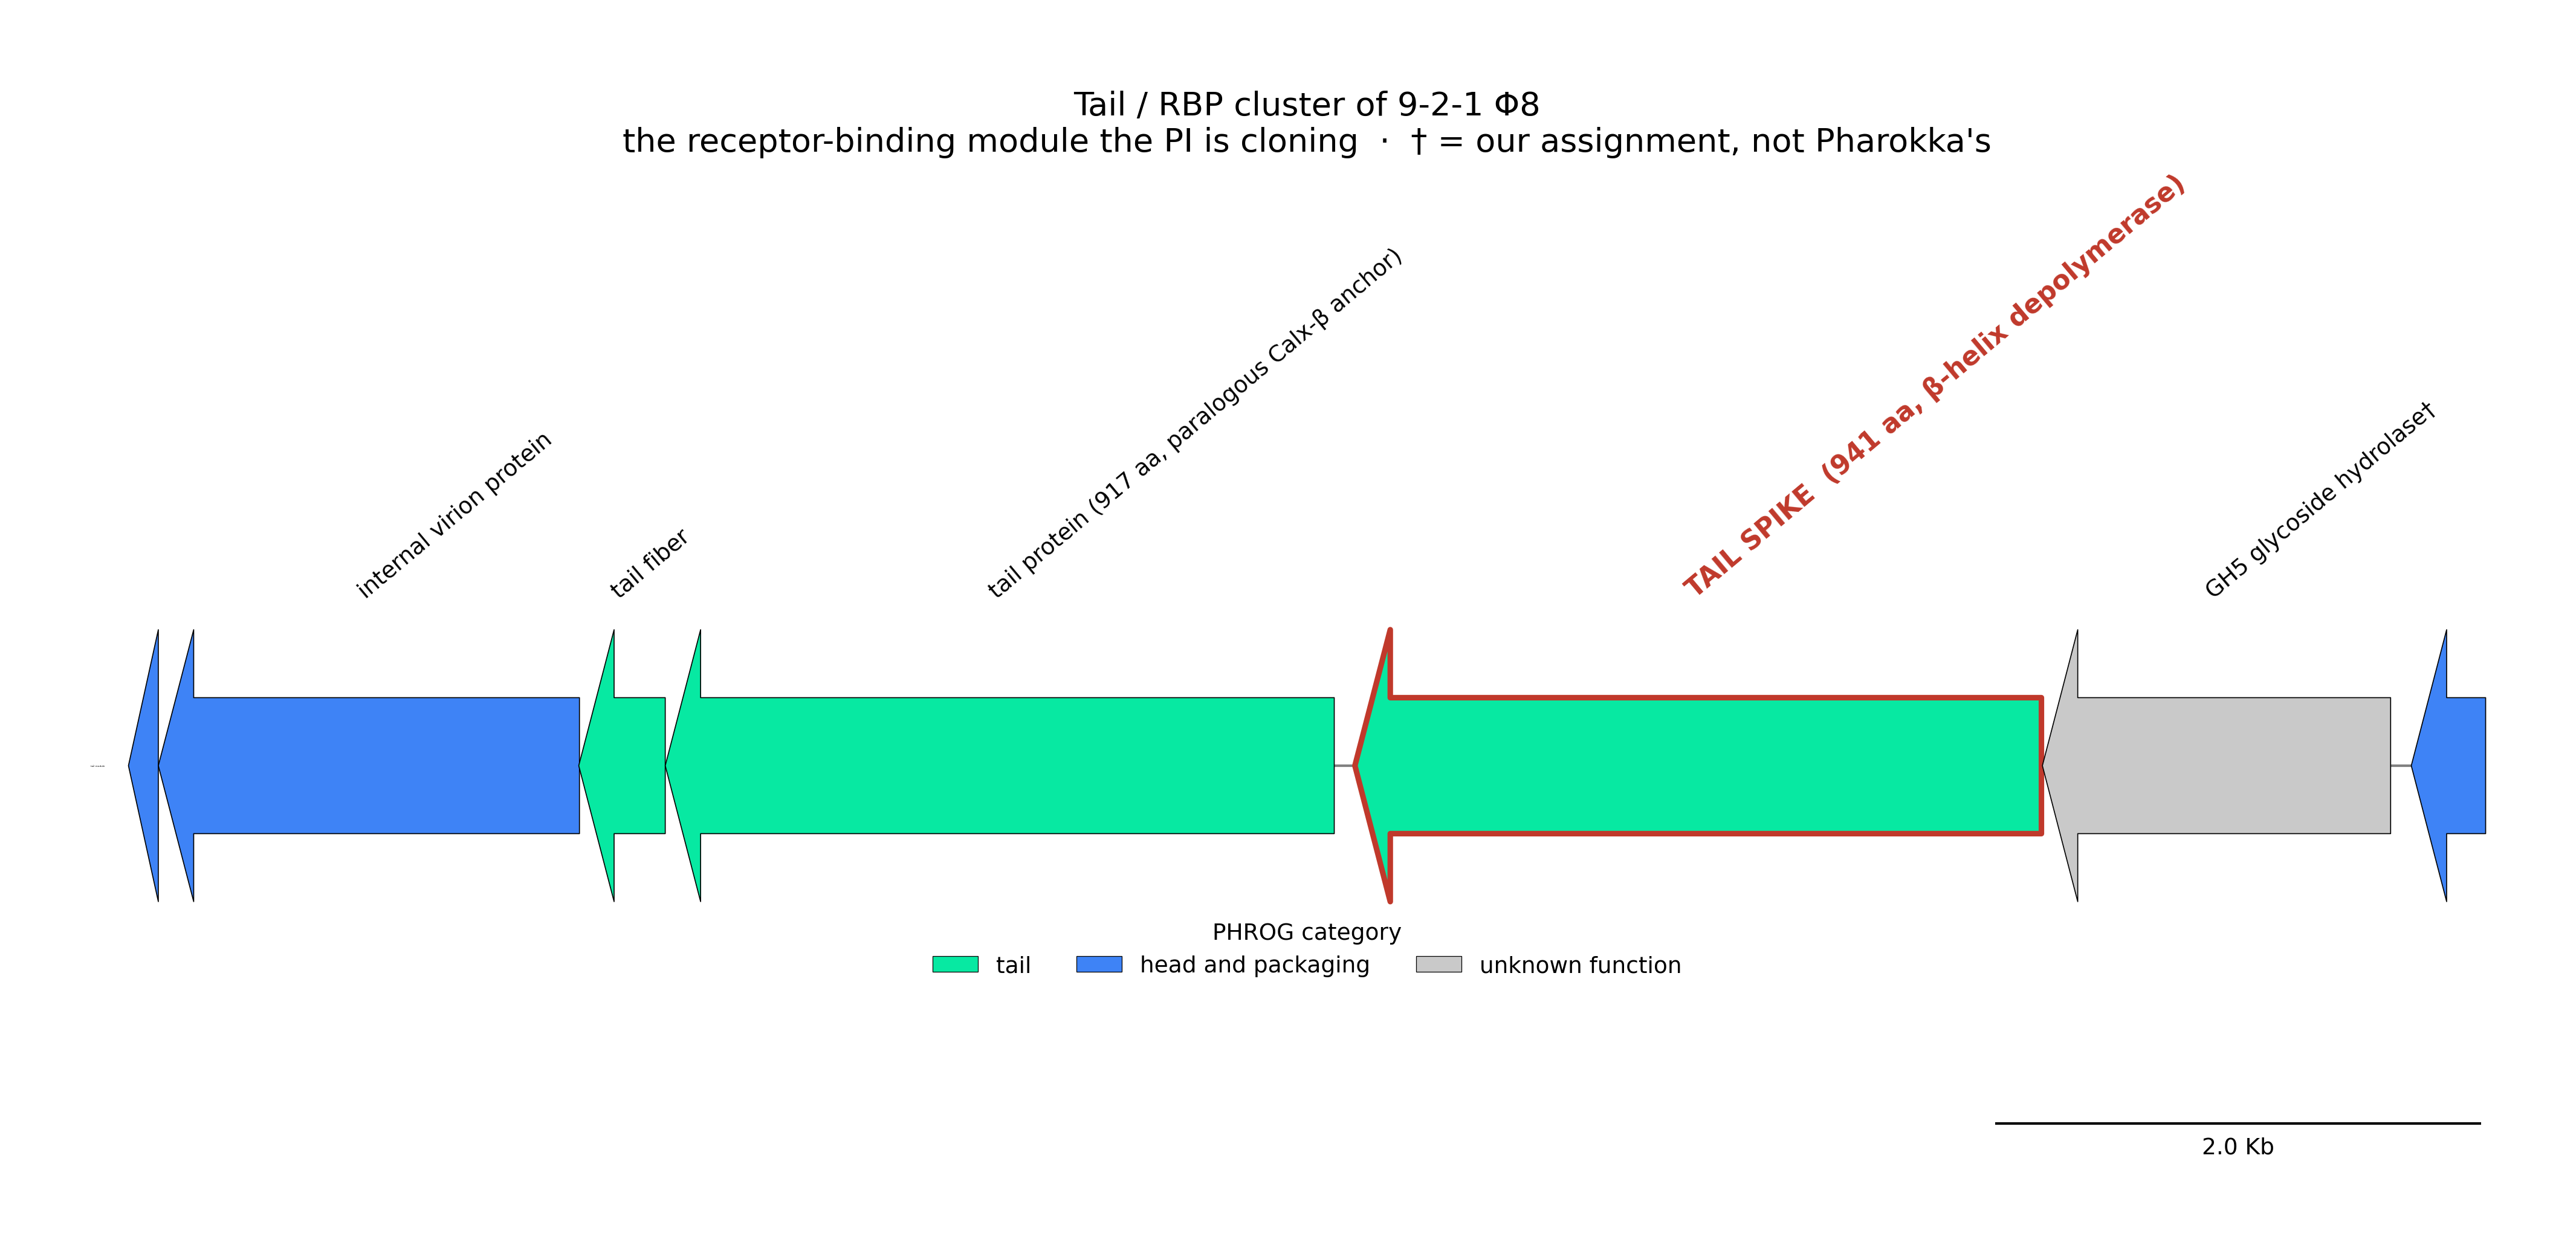
\includegraphics[width=0.98\textwidth,height=0.70\textheight,keepaspectratio]{../../code/output/0729_prof_figures/fig_phage_tail_module.png}\\
  {\scriptsize\color{muted} Numbering is the PI's \texttt{UUAIURNK\_}. The old 0708 genome map is
   mirrored — do not reuse it.}
\end{frame}

\begin{frame}{Backup 7 — enzymatic domains in full (incl.\ CDS\_0012 GH5)}
  \centering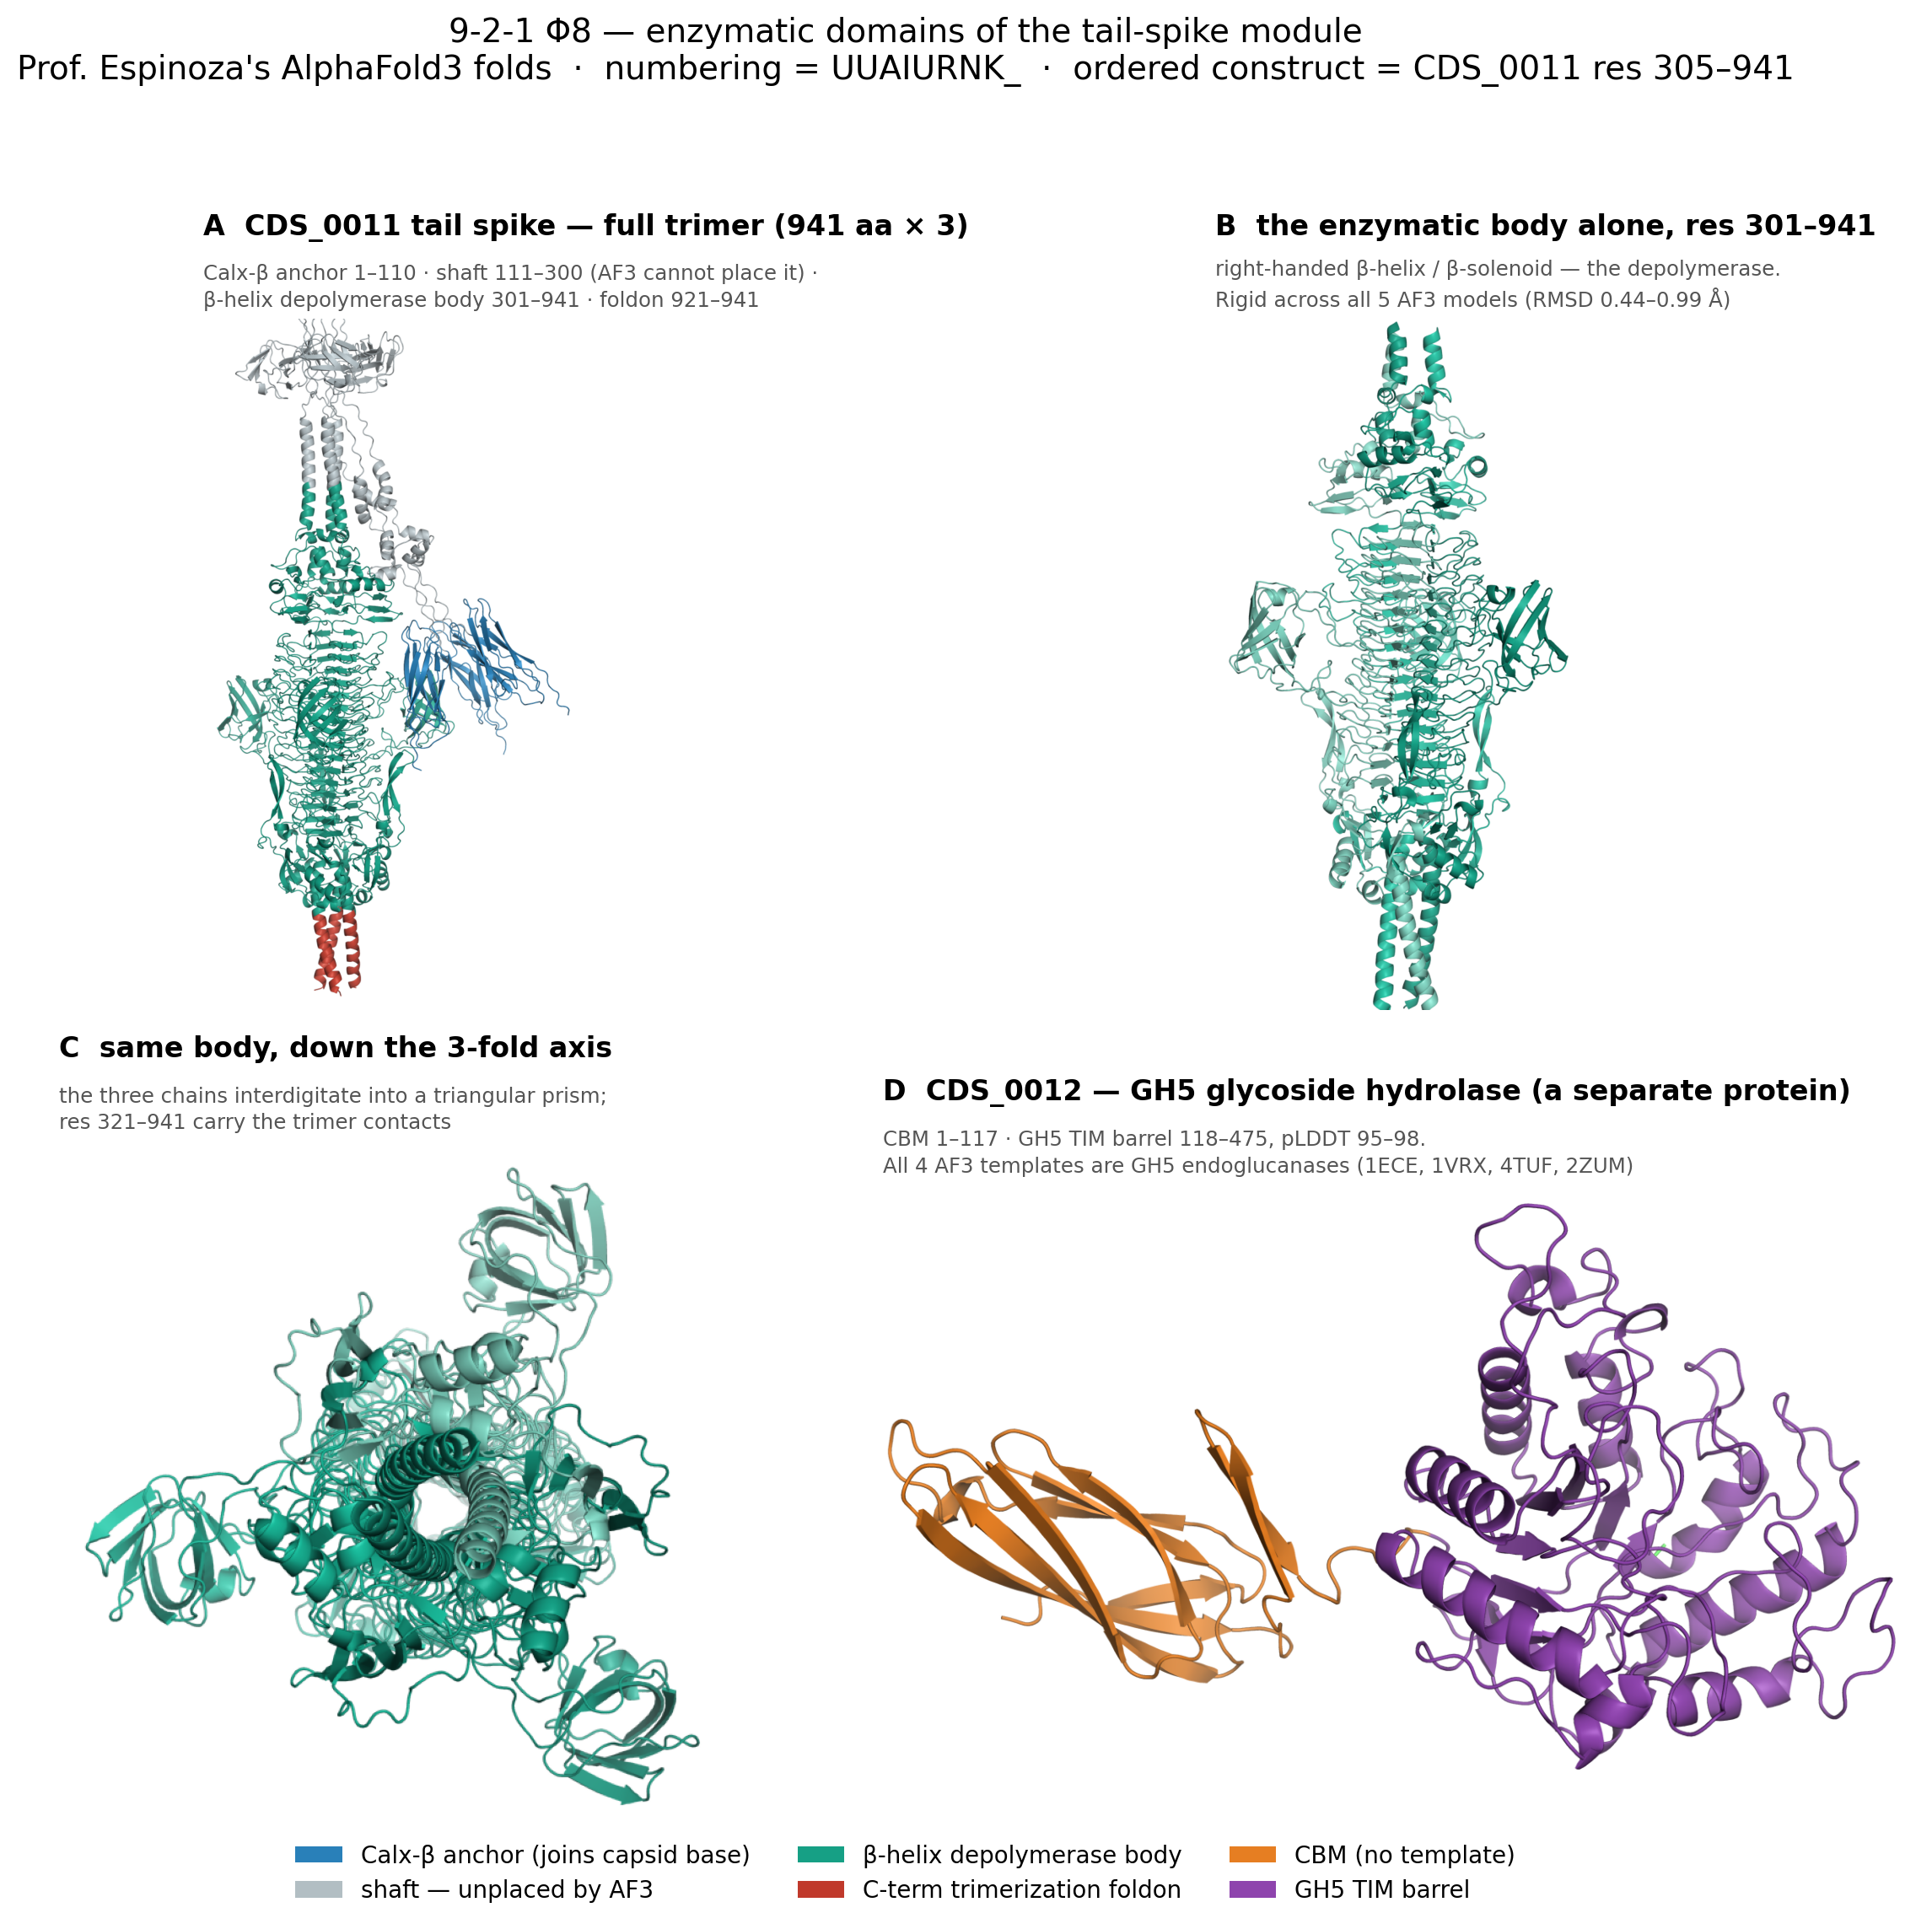
\includegraphics[width=0.68\textwidth,height=0.76\textheight,keepaspectratio]{../../code/output/0729_prof_figures/fig_enzymatic_domains.png}\\
  {\scriptsize\color{muted} Panel D is CDS\_0012 — a \textbf{separate protein}, not a domain of the
   tail spike.}
\end{frame}

\end{document}
"` prints the speaker script instead of the slides
\ifdefined\NOTESONLY \setbeameroption{show only notes}\setbeamerfont{note page}{size=\footnotesize} \fi

\begin{document}

% ---------------------------------------------------------------- 1. title
\begin{frame}[plain]
  \vspace{6pt}
  \begin{center}
    {\LARGE\bfseries Engineering the part that picks the host}\\[4pt]
    {\large Which gene, what it binds, where evolution comes in}
  \end{center}
  \vspace{4pt}
  \begin{center}
    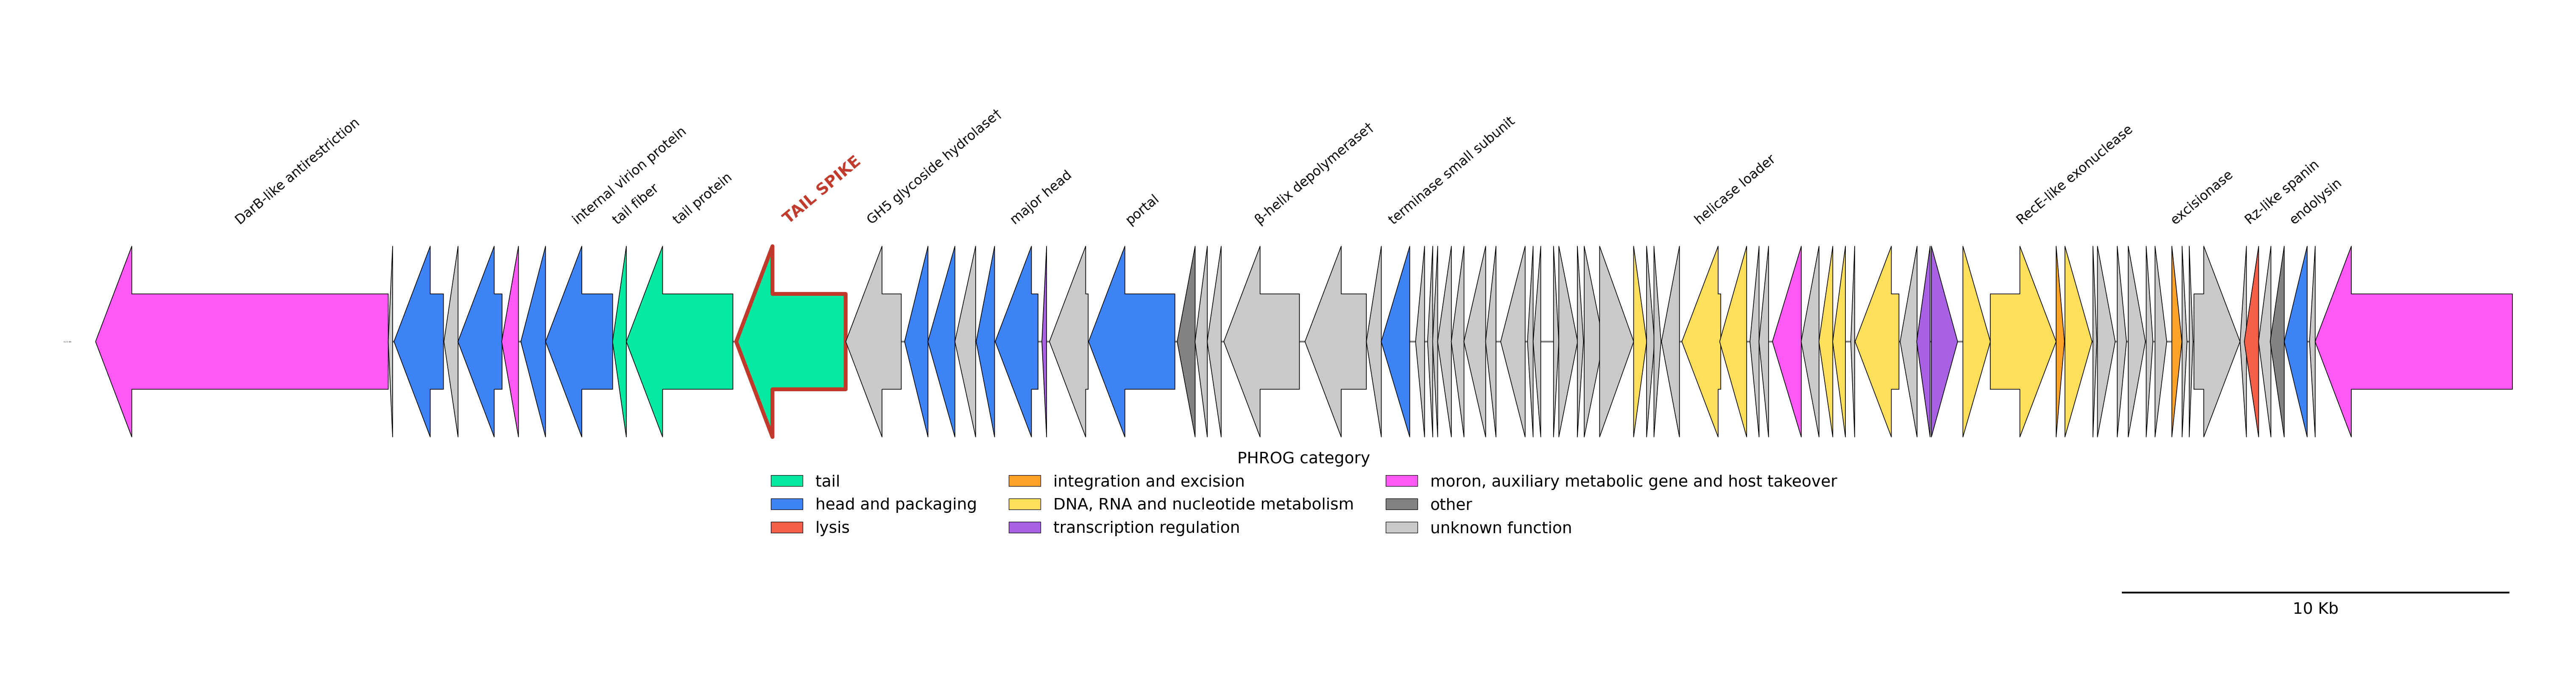
\includegraphics[width=0.95\textwidth]{fig/phage_map_banner.png}
  \end{center}
  \vspace{2pt}
  \begin{center}
  {\scriptsize\color{muted} Phage 9-2-1 $\Phi$8 — 62 kb, 80 genes — and three self-isolated
   \textit{Pseudomonas} strains\par
   \vspace{3pt}
   Chun-Yu (Alex) Chen \quad|\quad Phagenomics, Claremont CA \quad|\quad
   PI: J. Cesar Ignacio-Espinoza \quad|\quad 2026-08-21}
  \end{center}
  \note{
  Good evening. We are trying to build phage parts on purpose — to take the protein that decides which
  bacterium a phage can infect, and redesign it. Tonight: the two things you need before you can.\par
  ($\approx$18 s)}
\end{frame}

% ---------------------------------------------------------------- 2. context / goal
\begin{frame}[shrink=5]{We want to design the part, not just describe the phage}
  \begin{columns}[T,onlytextwidth]
    \begin{column}{0.53\textwidth}
      \footnotesize
      \begin{itemize}\setlength\itemsep{5pt}
        \item Phages hunt bacteria, and one phage usually infects \textbf{one strain} and ignores the
              next one over. Matching is done by \textbf{trial and error} today.
        \item Why now: \textcolor{cwzz}{\textbf{[AMR figure + source — Alex]}}. A phage is only useful
              if it hits the strain that is actually making someone sick.
        \item Our goal is a \textbf{part you can re-aim}: rebuild the receptor-binding protein so the
              same phage attacks a different strain.
        \item \textbf{We work on our own material} — local soil and water $\rightarrow$
              \textit{Pseudomonas} hosts and their phages, sequenced in house.
      \end{itemize}
      \vspace{4pt}
      \colorbox{accent!10}{\parbox{0.95\textwidth}{\centering\footnotesize
      \textbf{Tonight:} 5 isolates $\rightarrow$ \textbf{3 strains}, and one complete phage genome}}
    \end{column}
    \begin{column}{0.45\textwidth}
      \centering
      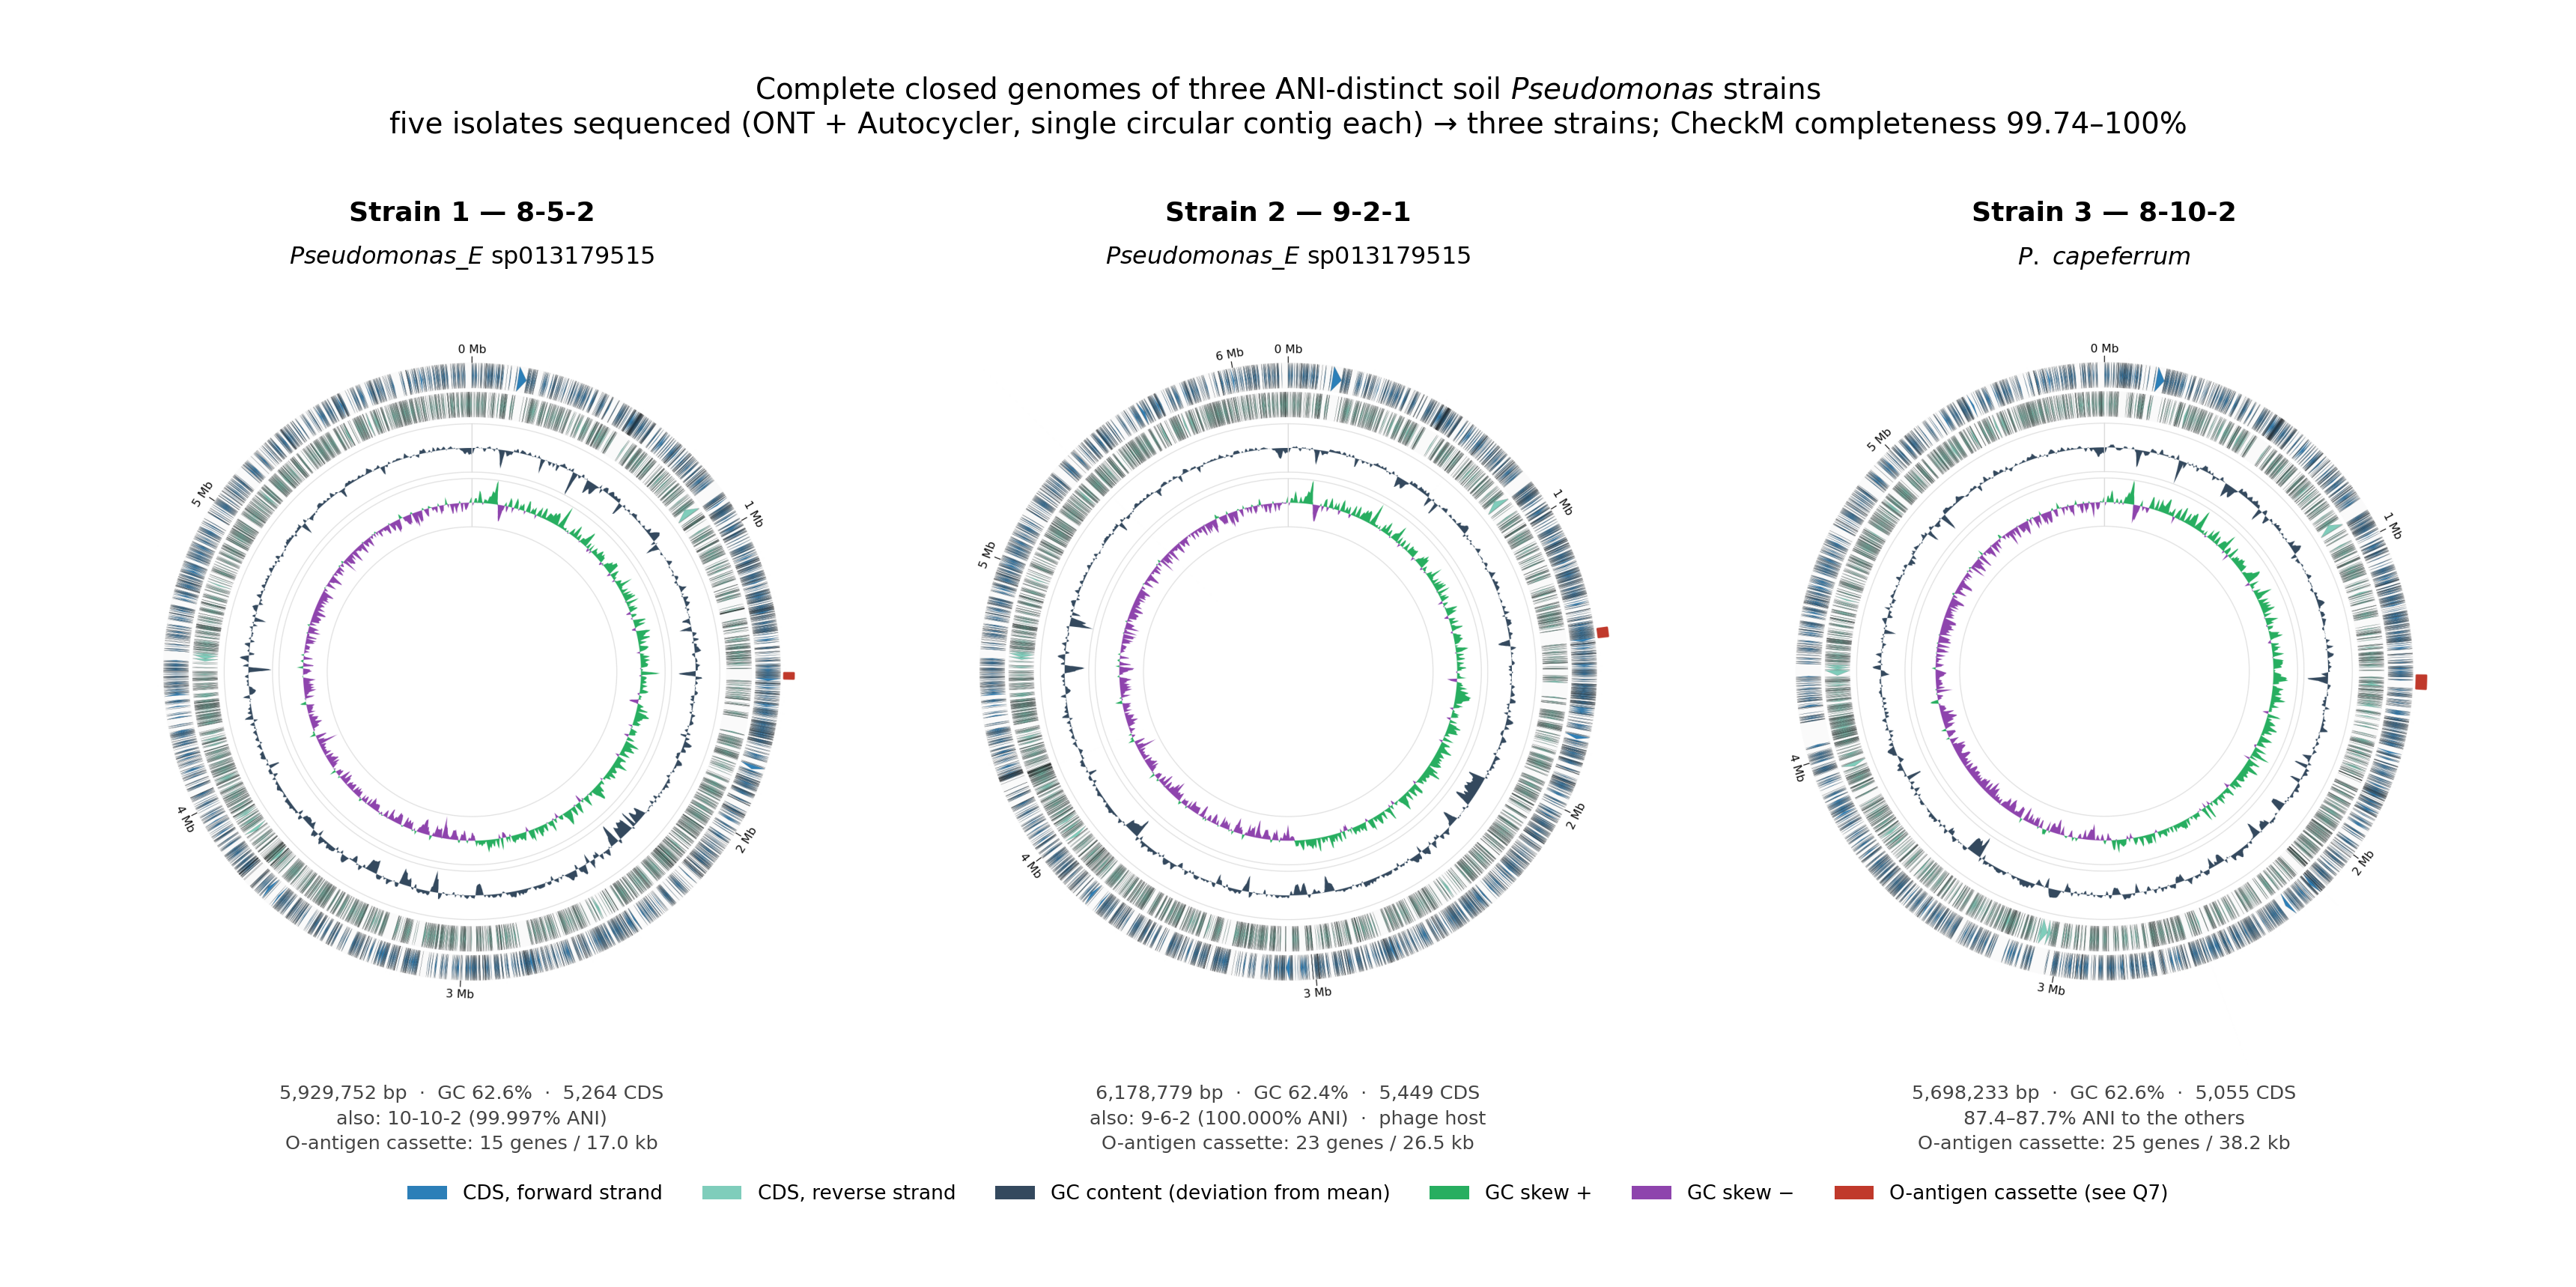
\includegraphics[width=0.98\textwidth]{../../code/output/0729_prof_figures/fig_bacterial_genomes.png}\\
      {\scriptsize\color{muted} three closed host genomes, 5.7–6.2 Mb}\\[5pt]
      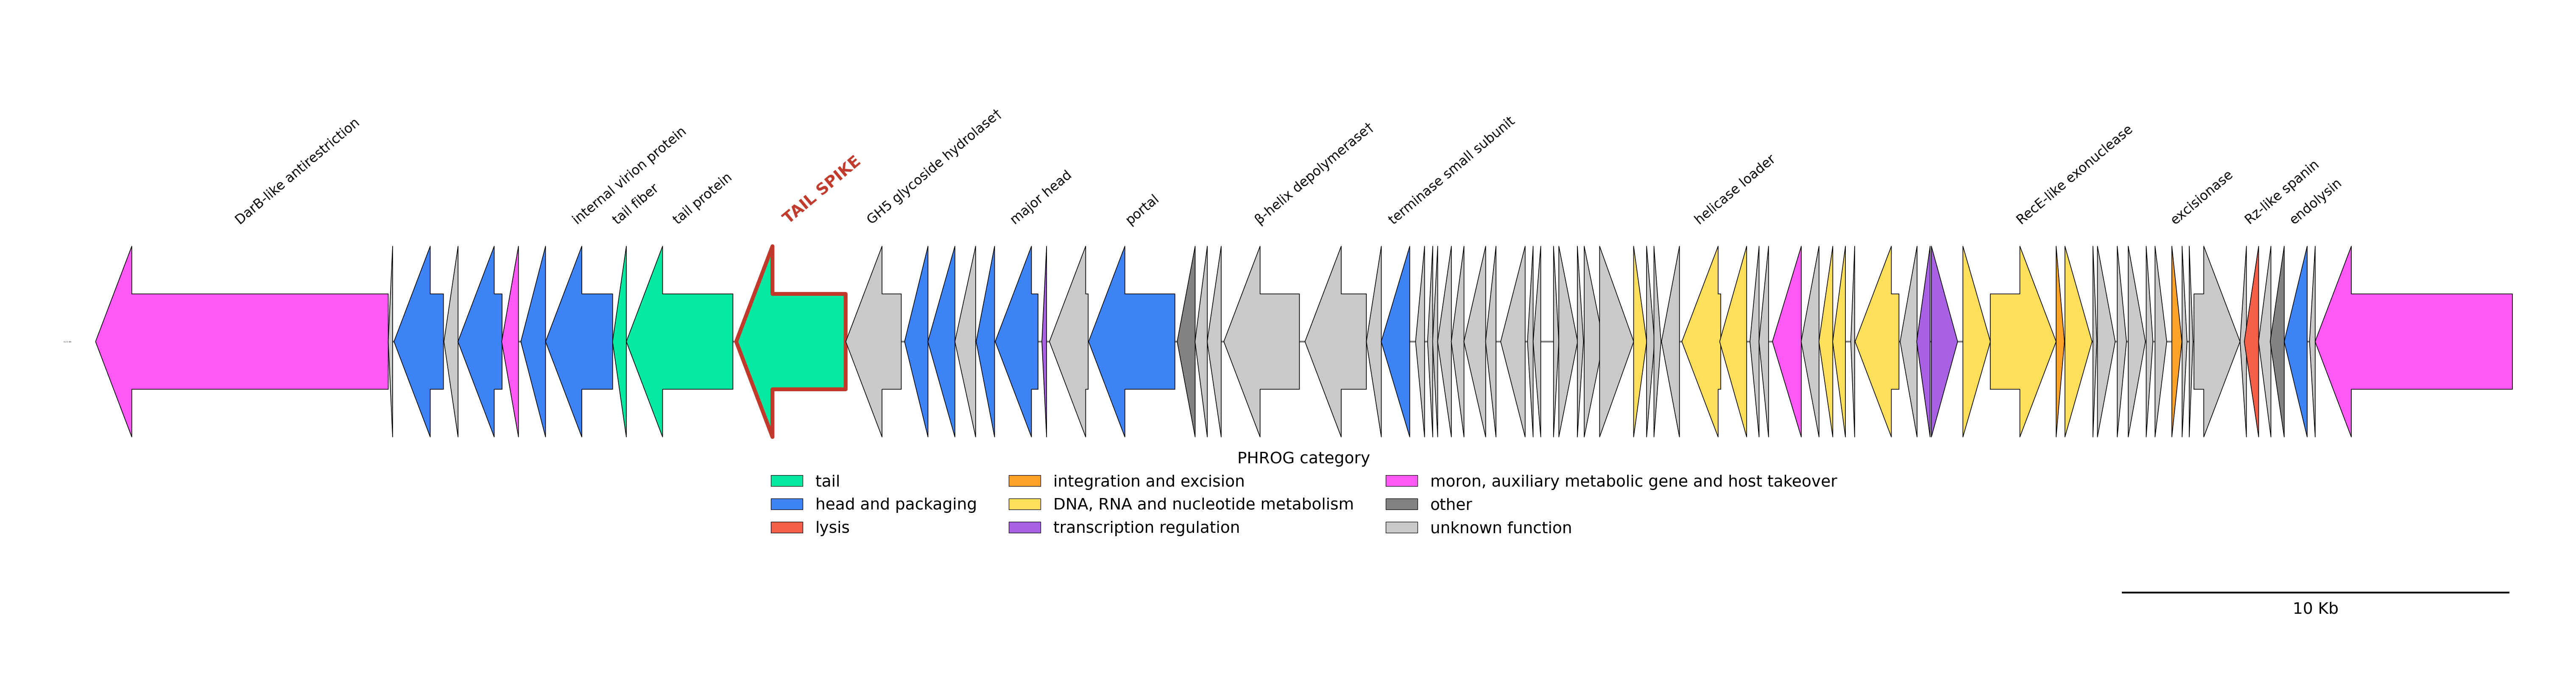
\includegraphics[width=0.98\textwidth]{fig/phage_map_banner.png}\\
      {\scriptsize\color{muted} the phage: 62 kb, 80 CDS, linear + 77 bp DTR}
    \end{column}
  \end{columns}
  \note{
  Phages hunt bacteria, and they are picky: one phage infects one strain and ignores the next one
  over. Today that match is trial and error.\par
  That matters right now — [AMR number, Alex fills in]. A phage is only useful if it hits the strain
  making someone sick.\par
  So our goal is not to describe a phage; it is to build a part you can re-aim — rebuild the
  receptor-binding protein so the same phage attacks a different strain.\par
  We work on our own material: local soil and water, Pseudomonas hosts and their phages, sequenced in
  house — five isolates, three strains, one complete phage genome.\par
  ($\approx$48 s)}
\end{frame}

% ---------------------------------------------------------------- 3. the design pipeline
\begin{frame}{The design loop — and where we actually are}
  \vspace{-2pt}
  \rqbox{Before you can redesign the targeting part: \textbf{which gene is it}, and \textbf{what must it recognise}?}
  \vspace{-2pt}
  \begin{center}
  \begin{tikzpicture}[
    font=\scriptsize,
    done/.style={draw=accent,line width=1.0pt,rounded corners=2pt,fill=accent!8,
                 text width=2.35cm,align=center,minimum height=1.8cm,inner sep=3pt},
    plan/.style={draw=muted,line width=0.9pt,dashed,rounded corners=2pt,fill=white,
                 text width=2.35cm,align=center,minimum height=1.8cm,inner sep=3pt},
    ar/.style={-{Stealth[length=4pt]},draw=muted,line width=0.7pt}]
    \node[done] (a) {\textbf{1. pick the gene}\\80 CDS $\rightarrow$ tail\\module: CDS\_0011,\\0012, 0024};
    \node[done,right=0.30cm of a] (b) {\textbf{2. define the\\target}\\fold it: what does\\it bind?};
    \node[plan,right=0.30cm of b] (c) {\textbf{3. learn from\\evolution}\\GH5 tree $\rightarrow$\\ancestral enzymes};
    \node[plan,right=0.30cm of c] (d) {\textbf{4. build\\variants}\\3 at Twist\\+ ancestral GH5};
    \node[plan,right=0.30cm of d] (e) {\textbf{5. test}\\fiber + depolymerase\\\emph{in trans}, 3 strains};
    \draw[ar] (a)--(b); \draw[ar] (b)--(c); \draw[ar] (c)--(d); \draw[ar] (d)--(e);
    \draw[ar,draw=muted,dashed] (e.south) -- ++(0,-0.35) -| node[pos=0.25,below,font=\scriptsize\color{muted}]{design rules} (c.south);
  \end{tikzpicture}
  \end{center}
  \vspace{2pt}
  {\scriptsize\color{muted} \tikz[baseline=-0.5ex]\draw[accent,line width=1pt,fill=accent!8] (0,0) rectangle (1.6ex,1.6ex);
   solid = has data \quad
   \tikz[baseline=-0.5ex]\draw[muted,dashed,line width=0.9pt] (0,0) rectangle (1.6ex,1.6ex);
   dashed = in progress / proposed \quad|\quad the next two slides are steps 1 and 2}
  \note{
  Here is the loop. Step one, pick the gene: of 80 genes the structural module narrows it to a
  handful — the tail spike, the GH5 beside it, and a depolymerase the annotator missed.\par
  Step two, define the target — you cannot redesign a binder without knowing what it binds.\par
  Step three is where evolution comes in. The tail spike decides who is recognised; the depolymerase
  decides what can be cut open. So we build a tree over all GH5 sequences and reconstruct ancestral
  enzymes — proteins from different points in evolution, not random mutants. Stated caveat: this
  assumes affinity tracks infection.\par
  Step four, build them: three constructs are at Twist, ancestral enzymes next. Step five, combine
  fiber and depolymerase in trans on our three strains, and feed that back as design rules.\par
  Solid boxes have data; dashed ones do not. The next two slides are steps one and two.\par
  ($\approx$62 s)}
\end{frame}

% ---------------------------------------------------------------- 4. result 1 — the part
\begin{frame}[shrink=5]{Steps 1--2: a $\beta$-helix depolymerase — the target is a sugar}
  \begin{columns}[T,onlytextwidth]
    \begin{column}{0.30\textwidth}
      \centering
      \includegraphics[height=0.60\textheight]{../../code/output/0729_prof_figures/panels/cds0011_trimer_domains.png}\\[2pt]
      {\scriptsize\color{muted} CDS\_0011 trimer, 941 aa $\times$ 3\par
       grey shaft \textbullet\ blue anchor\par
       \textcolor{accent}{\textbf{teal body}} \textbullet\ red foldon}
    \end{column}
    \begin{column}{0.68\textwidth}
      \footnotesize
      \begin{itemize}\setlength\itemsep{5pt}
        \item Right-handed \textbf{$\beta$-helix}, one rung every \textbf{15–18 residues} — the
              signature of a polysaccharide depolymerase. \textbf{This part cuts sugar}, so its target
              is the surface sugar, not a protein.
        \item The domain map is what makes it \textbf{engineerable}: pLDDT 88–94, and the body
              (res 301–941) is rigid to \textbf{0.44–0.99 \AA} across five models — that boundary is
              exactly where our construct starts (res 305).
        \item The protein--protein hypothesis was tested first \textbf{and failed}:
      \end{itemize}
      \vspace{1pt}
      \begin{center}
        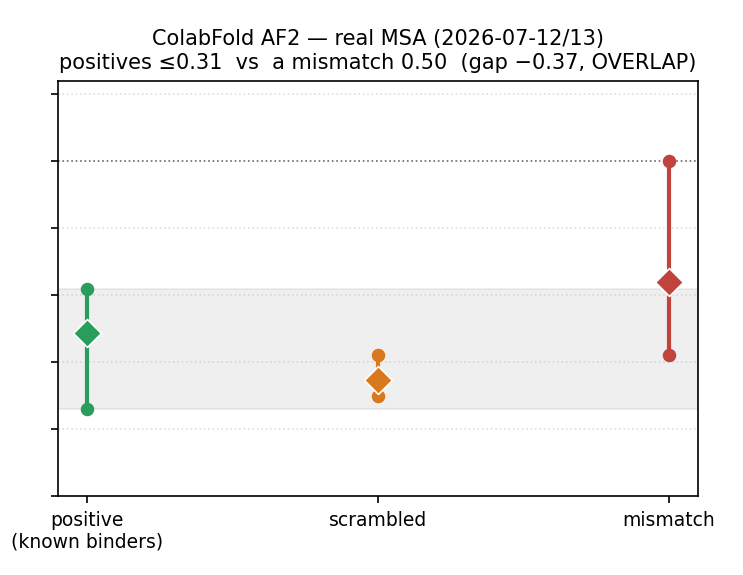
\includegraphics[height=0.25\textheight]{fig/binding_controls_af2.png}\\
        {\scriptsize\color{muted} positives ipTM $\leq$ 0.31 vs a mismatched pair 0.50 — no signal}
      \end{center}
    \end{column}
  \end{columns}
  \note{
  Steps one and two on one slide. This is the tail spike, 941 residues, a trimer: grey shaft AlphaFold
  cannot place, blue anchor into the capsid, teal working body.\par
  That body is a right-handed beta helix, one rung every 15 to 18 residues — the signature of a
  depolymerase. So the part cuts sugar, and its target is the surface sugar, not a protein.\par
  It is also engineerable: the body from residue 301 is rigid, under one angstrom across five models,
  and that boundary is exactly where our construct starts.\par
  And we tested the protein-protein hypothesis first — docking gave positives at 0.31 and a mismatch
  at 0.50. No discriminating power, so we retired that screen.\par
  ($\approx$57 s)}
\end{frame}

% ---------------------------------------------------------------- 5. result 2 — the target varies
\begin{frame}[shrink=5]{The target is different in every strain — that is the handle}
  \vspace{1pt}
  \footnotesize Same \texttt{ihfB}-flanked slot, different cargo
   \ \textcolor{muted}{(grey ribbons = homology)}\normalsize
  \vspace{1pt}
  \begin{center}
    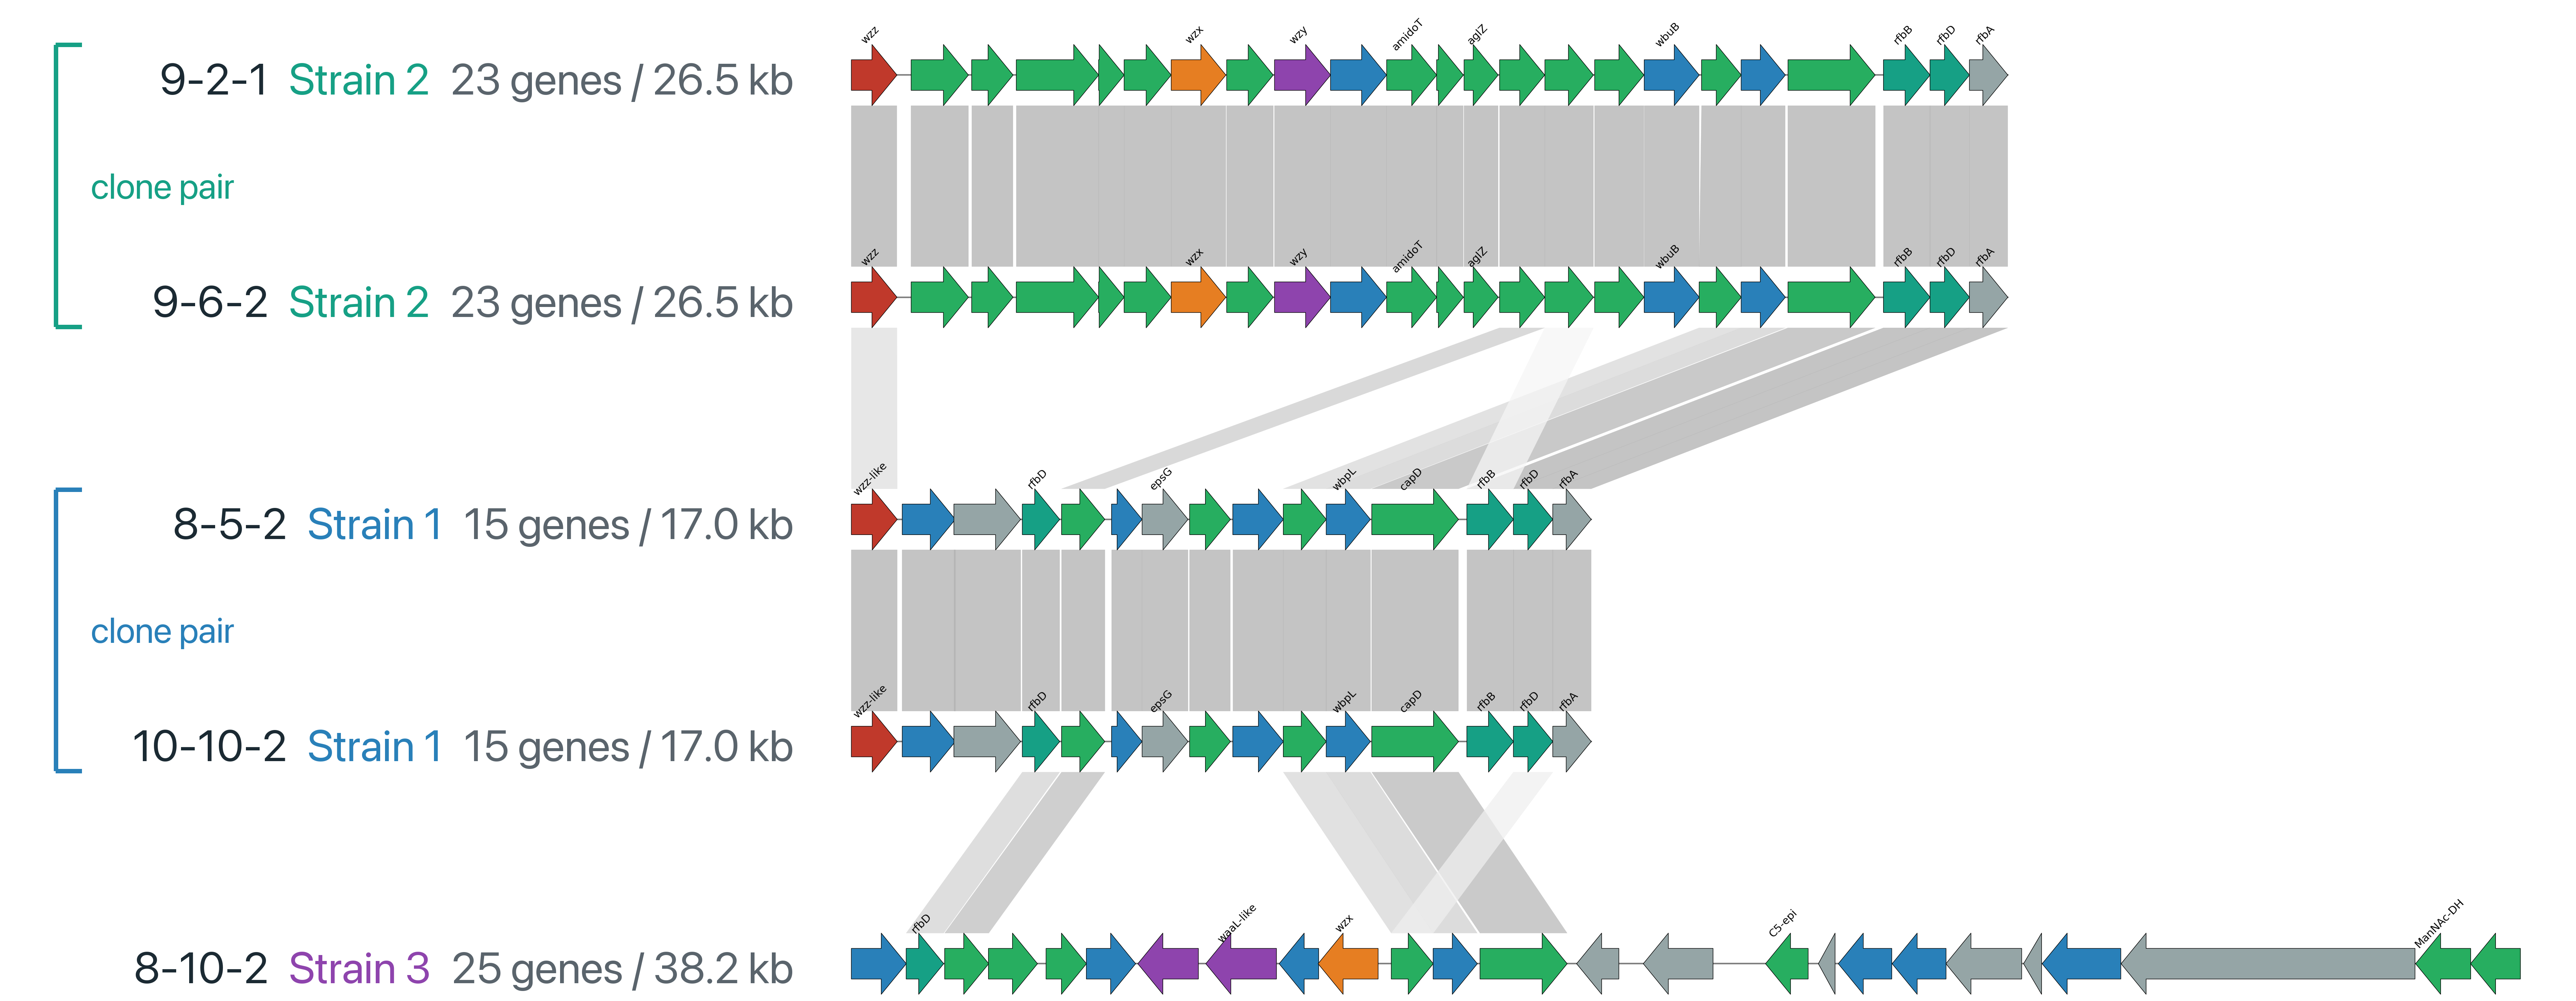
\includegraphics[width=0.95\textwidth,height=0.54\textheight,keepaspectratio]{fig/oantigen_tracks_labeled.png}
  \end{center}
  \vspace{-4pt}
  \begin{center}\tiny
    \chip{cwzz}{chain-length regulator}\quad\chip{cwzx}{flippase (wzx)}\quad\chip{cwzy}{polymerase (wzy)}\quad
    \chip{cgt}{glycosyltransferase}\quad\chip{crha}{dTDP-rhamnose}\quad\chip{cnuc}{nucleotide-sugar}\quad
    \chip{cother}{unassigned}
  \end{center}
  \vspace{1pt}
  {\footnotesize \textbf{4 of 45 clusters shared by all three} — generic sugar chemistry only, no
   shared assembly machinery. \textcolor{muted}{Control: clone pairs 100.0\% identical.}}
  \note{
  If the part reads a sugar, does that sugar differ between strains? That difference is the handle a
  redesigned part would turn.\par
  Five tracks: two Strain 2 clones, two Strain 1 clones, Strain 3; arrows are genes, grey ribbons are
  homology. Control first: inside each clone pair all 23 and all 15 genes are identical. ANI
  saturates, so this had to be measured.\par
  Across strains the links are sparse and crossed — of 45 clusters only four are shared, all generic
  sugar chemistry, no shared flippase, polymerase or chain-length regulator.\par
  Three strains, three targets. This phage should not plaque on the other two, and a re-aimed part is
  what would change that.\par
  ($\approx$57 s)}
\end{frame}

% ---------------------------------------------------------------- 6. close
\begin{frame}[shrink=5]{Where the loop stands}
  \begin{columns}[T,onlytextwidth]
    \begin{column}{0.50\textwidth}
      \small
      \textcolor{accent}{\textbf{Conclusion}}\\
      We know \textbf{which gene} to engineer and \textbf{what it must recognise}: the tail-spike
      depolymerase, against a strain-specific O-antigen — and our three strains give three different
      targets.
      \vspace{6pt}

      \textcolor{accent}{\textbf{Limitation}}\\
      Steps 3–5 are \textbf{not results yet}: the GH5 ancestral reconstruction is still being built,
      the constructs are not expressed, and the cross-strain plaque assay was run July 4 but the data
      is not in our hands. It also assumes affinity tracks infection. No serotyping tool exists for
      this taxon, so we cannot name an O-type.
      \vspace{6pt}

      \textcolor{accent}{\textbf{Next three months}}\\
      Recover that readout; express the three constructs; reconstruct ancestral GH5 enzymes and test
      fiber $+$ depolymerase \emph{in trans} on the three strains. The tail spike also has a
      15,775-sequence alignment — enough for a conservation profile on the structure.
    \end{column}
    \begin{column}{0.48\textwidth}
      \centering
      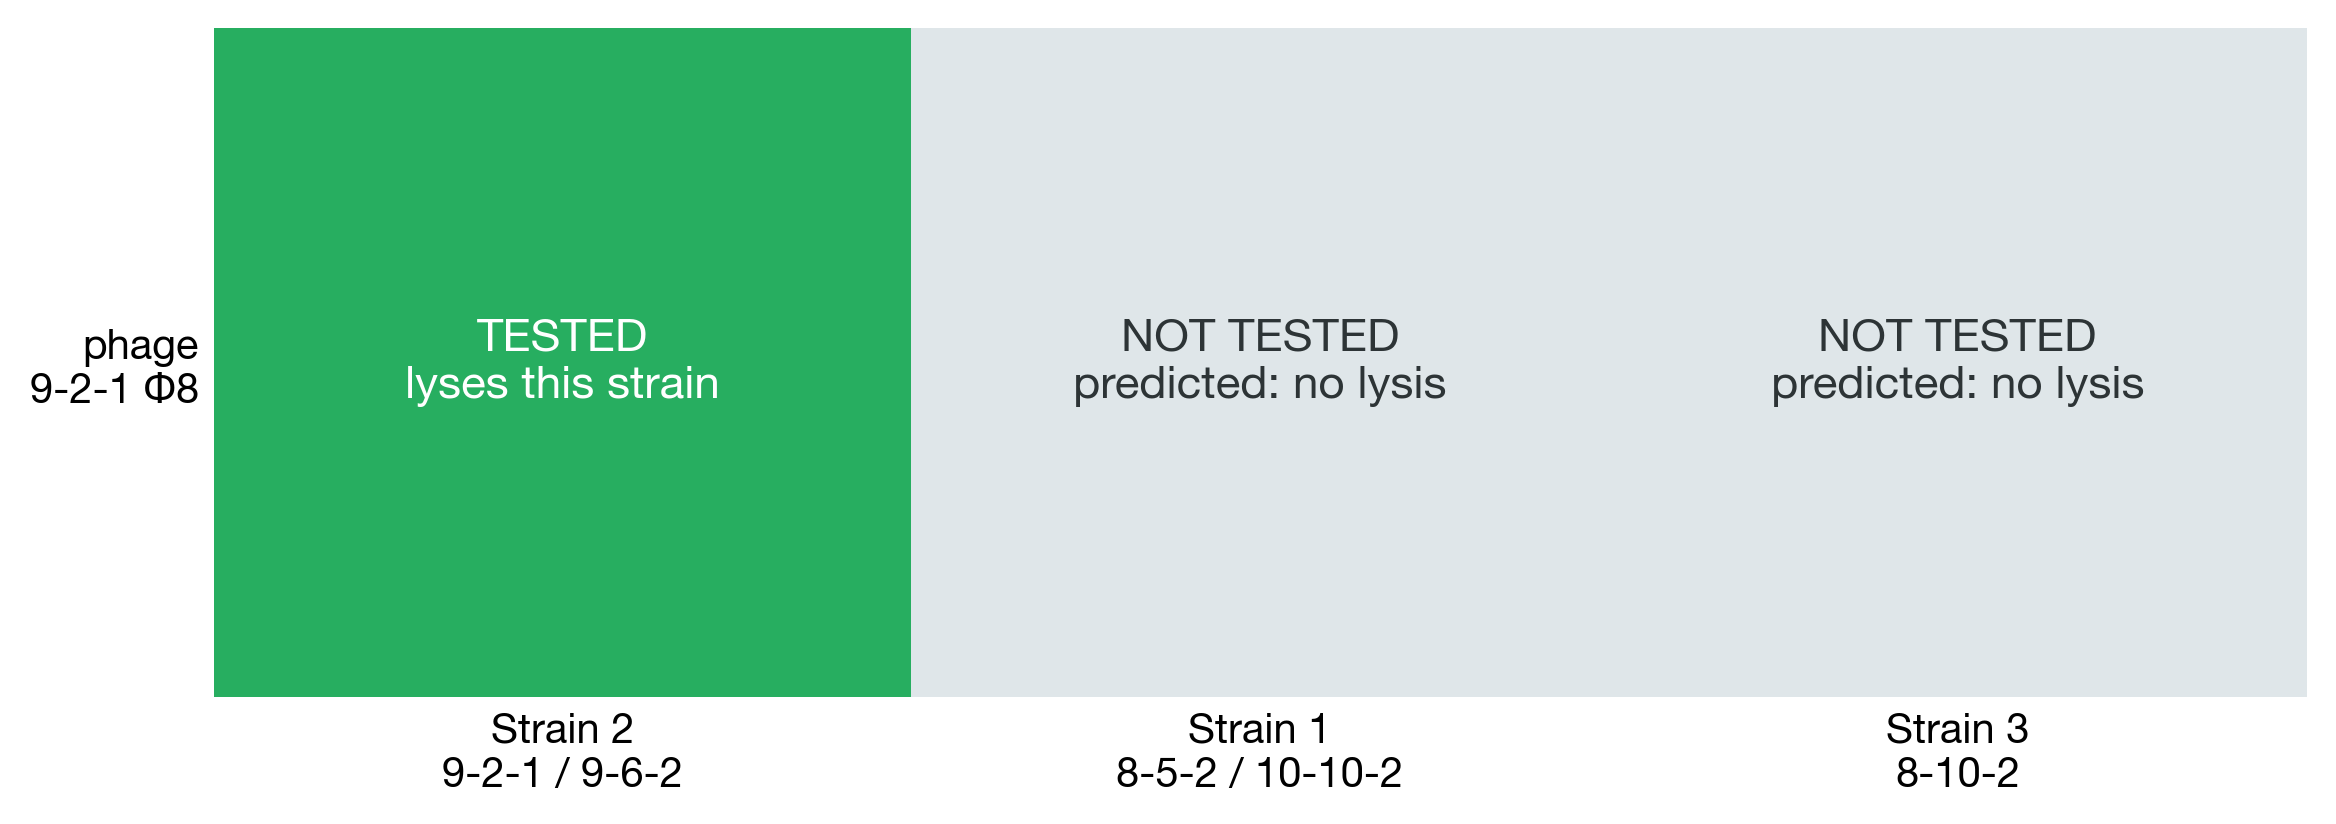
\includegraphics[width=\textwidth]{fig/hostrange_cells.png}\\[3pt]
      {\scriptsize\color{muted} only Strain 2 has actually been challenged; the grey cells are
       predictions, and the July 4 assay reads them out}\\[8pt]
      \begin{flushleft}\scriptsize
      \textcolor{accent}{\textbf{1. pick the gene}} — done\\
      \textcolor{accent}{\textbf{2. define the target}} — done\\
      \textcolor{muted}{\textbf{3. ancestral GH5 enzymes} — PI building the tree}\\
      \textcolor{muted}{\textbf{4. build} — 3 constructs at Twist}\\
      \textcolor{muted}{\textbf{5. test} — \emph{in trans}, waiting on the July 4 readout}
      \end{flushleft}
    \end{column}
  \end{columns}
  \vspace{5pt}
  \begin{center}\large\bfseries We now know which part to rebuild and what it has to grip — the
   ancestral variants are the next lever.\end{center}
  \note{
  Where the loop stands. We know which gene to engineer and what it must recognise — the tail-spike
  depolymerase against a strain-specific O-antigen — and three strains give three targets.\par
  The limitation is honest: steps three to five are not results — the GH5 tree is still being built,
  the constructs are not expressed, and the July fourth plaque data is not in our hands. And no
  serotyping tool exists for this taxon, so we cannot name an O-type.\par
  Next three months: recover that readout, express the constructs, and reconstruct ancestral GH5
  enzymes — then measure how proteins from different points in evolution behave with the fiber, in
  trans, on the three strains.\par
  We know which part to rebuild and what it has to grip. The ancestral variants are the next lever.\par
  ($\approx$58 s — stop here, not on a thank-you slide)}
\end{frame}

% ================================================================ backup
\begin{frame}[plain]
  \vspace{1.2cm}\centering{\Large\bfseries Backup}\\[4pt]{\color{muted} not shown unless asked}
\end{frame}

\begin{frame}{Backup 1 — gene selection and the constructs}
  \small
  \begin{itemize}\setlength\itemsep{5pt}
    \item Structural module, in canonical podovirus order: portal (CDS\_0020) $\rightarrow$ major
          capsid (0017) $\rightarrow$ adaptors $\rightarrow$ \textbf{tail spike (0011)} $\rightarrow$
          tail (0010) $\rightarrow$ fiber (0009).
    \item \textbf{CDS\_0024 is a second $\beta$-helix depolymerase} (rung 22–24) that Pharokka called
          ``hypothetical''; the de-novo RBP classifier found it at score 0.998.
    \item \textbf{CDS\_0012 is a GH5 glycoside hydrolase} — a separate protein, not a domain of the
          tail spike; all four AF3 templates are GH5 endoglucanases.
    \item Ordered from Twist 2026-07-27, all in pET-28a(+) with N-terminal His6:
          CDS\_0011 res \textbf{305–941} (the rigid body), CDS\_0010 res 105–917,
          CDS\_0012 res 117–477.
    \item CDS\_0010 is an \textbf{unknown protein} — the glycosidase call was withdrawn 2026-07-29;
          it is being expressed for functional characterisation.
  \end{itemize}
\end{frame}

\begin{frame}{Backup 2 — how the locus was pulled, how orthology was called}
  \small
  \begin{itemize}\setlength\itemsep{5pt}
    \item Anchor, identical in all five genomes: 30S ribosomal protein S1 $\rightarrow$ \texttt{ihfB}
          $\rightarrow$ LPS assembly protein A $\rightarrow$ MBL-fold hydrolase $\rightarrow$
          \textbf{cassette starts}. \texttt{ihfB} is the canonical upstream flank of the
          \textit{Pseudomonas} OSA cluster in the literature.
    \item Orthology = MMseqs2 clustering, $\geq$30\% identity / $\geq$50\% coverage.
          \textbf{Product names cannot be used}: the chain-length regulators of Strain 1 and Strain 2
          carry different Bakta labels but are homologous by sequence.
    \item Locus sizes: Strain 2 = 23 genes / 26.5 kb \textbullet\ Strain 1 = 15 / 17.0 kb \textbullet\
          Strain 3 = 25 / 38.2 kb.
    \item The cross-strain best-hit numbers (9/23, 10/23, 6/15) are one-directional best hits at a
          looser cutoff and are not meant to reconcile with the 45/4 cluster counts.
  \end{itemize}
\end{frame}

\begin{frame}{Backup 3 — cluster matrix, 45 clusters $\times$ 3 strains}
  \centering
  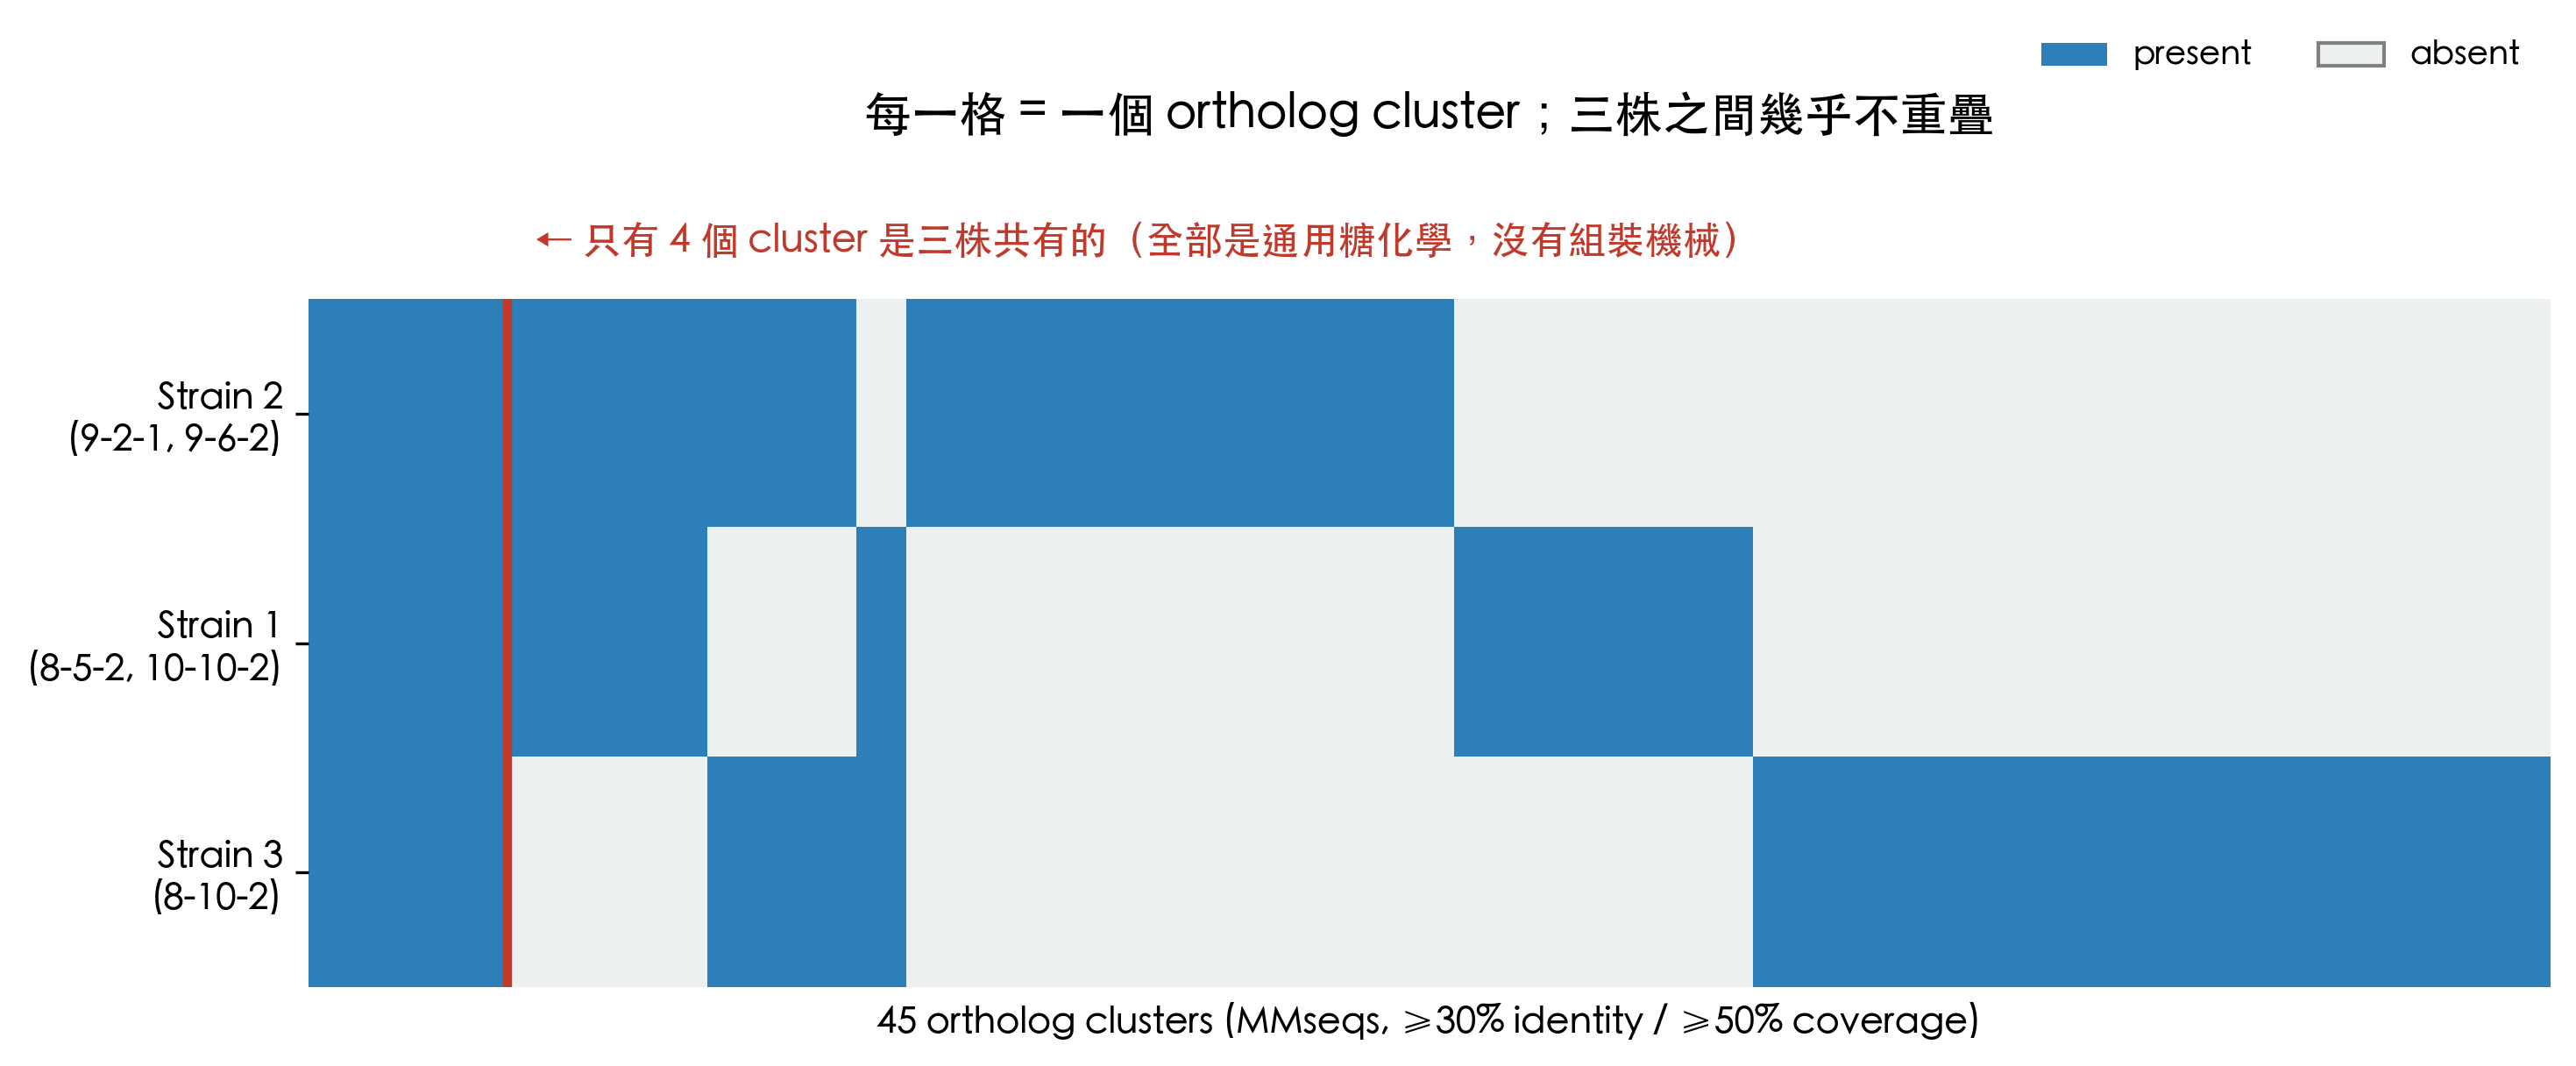
\includegraphics[width=0.86\textwidth,height=0.74\textheight,keepaspectratio]{../../code/output/0727_o_antigen_comparison/fig2_cluster_presence.png}
\end{frame}

\begin{frame}{Backup 4 — limitations in full}
  \small
  \begin{itemize}\setlength\itemsep{5pt}
    \item \textbf{Variable $\neq$ specificity-determining.} An earlier plan to read specificity off
          metagenomic variable regions was rejected in our own review: metagenome sequences carry no
          host labels, so specificity-determining positions cannot be identified that way. The
          15,775-sequence alignment (tail spike, CDS\_0011) supports a \textbf{conservation profile}
          — not ``these residues set the host range''. The ancestral reconstruction the PI is building
          is a separate thing: a tree over \textbf{all GH5 sequences} (CDS\_0012), whose ancestral
          enzymes get expressed and challenged \emph{in trans}, under the stated caveat that
          affinity $\sim$ binding $\sim$ infection.
    \item \textbf{Do not say Strain 1 lacks a flippase or polymerase} — Bakta assigns no Pfam/InterPro
          to those two genes; confirming them needs InterProScan.
    \item \textbf{The sugar structure has not been measured} — gene content is not structure; that
          needs LPS extraction and mass spectrometry.
    \item \textbf{The $\beta$-helix has no named structural homolog yet} — no foldseek or DALI run.
    \item \textbf{Taxonomy}: the virion module is podovirus-like, but reciprocal best hits against T7,
          $\varphi$KMV and KP32 are $\approx$0 and the genome carries an excisionase; \textit{terL} is
          unannotated, so formal taxonomy cannot be run. ``T7-like'' is an organizational analogy only.
  \end{itemize}
\end{frame}

\begin{frame}{Backup 5 — the three host genomes}
  \centering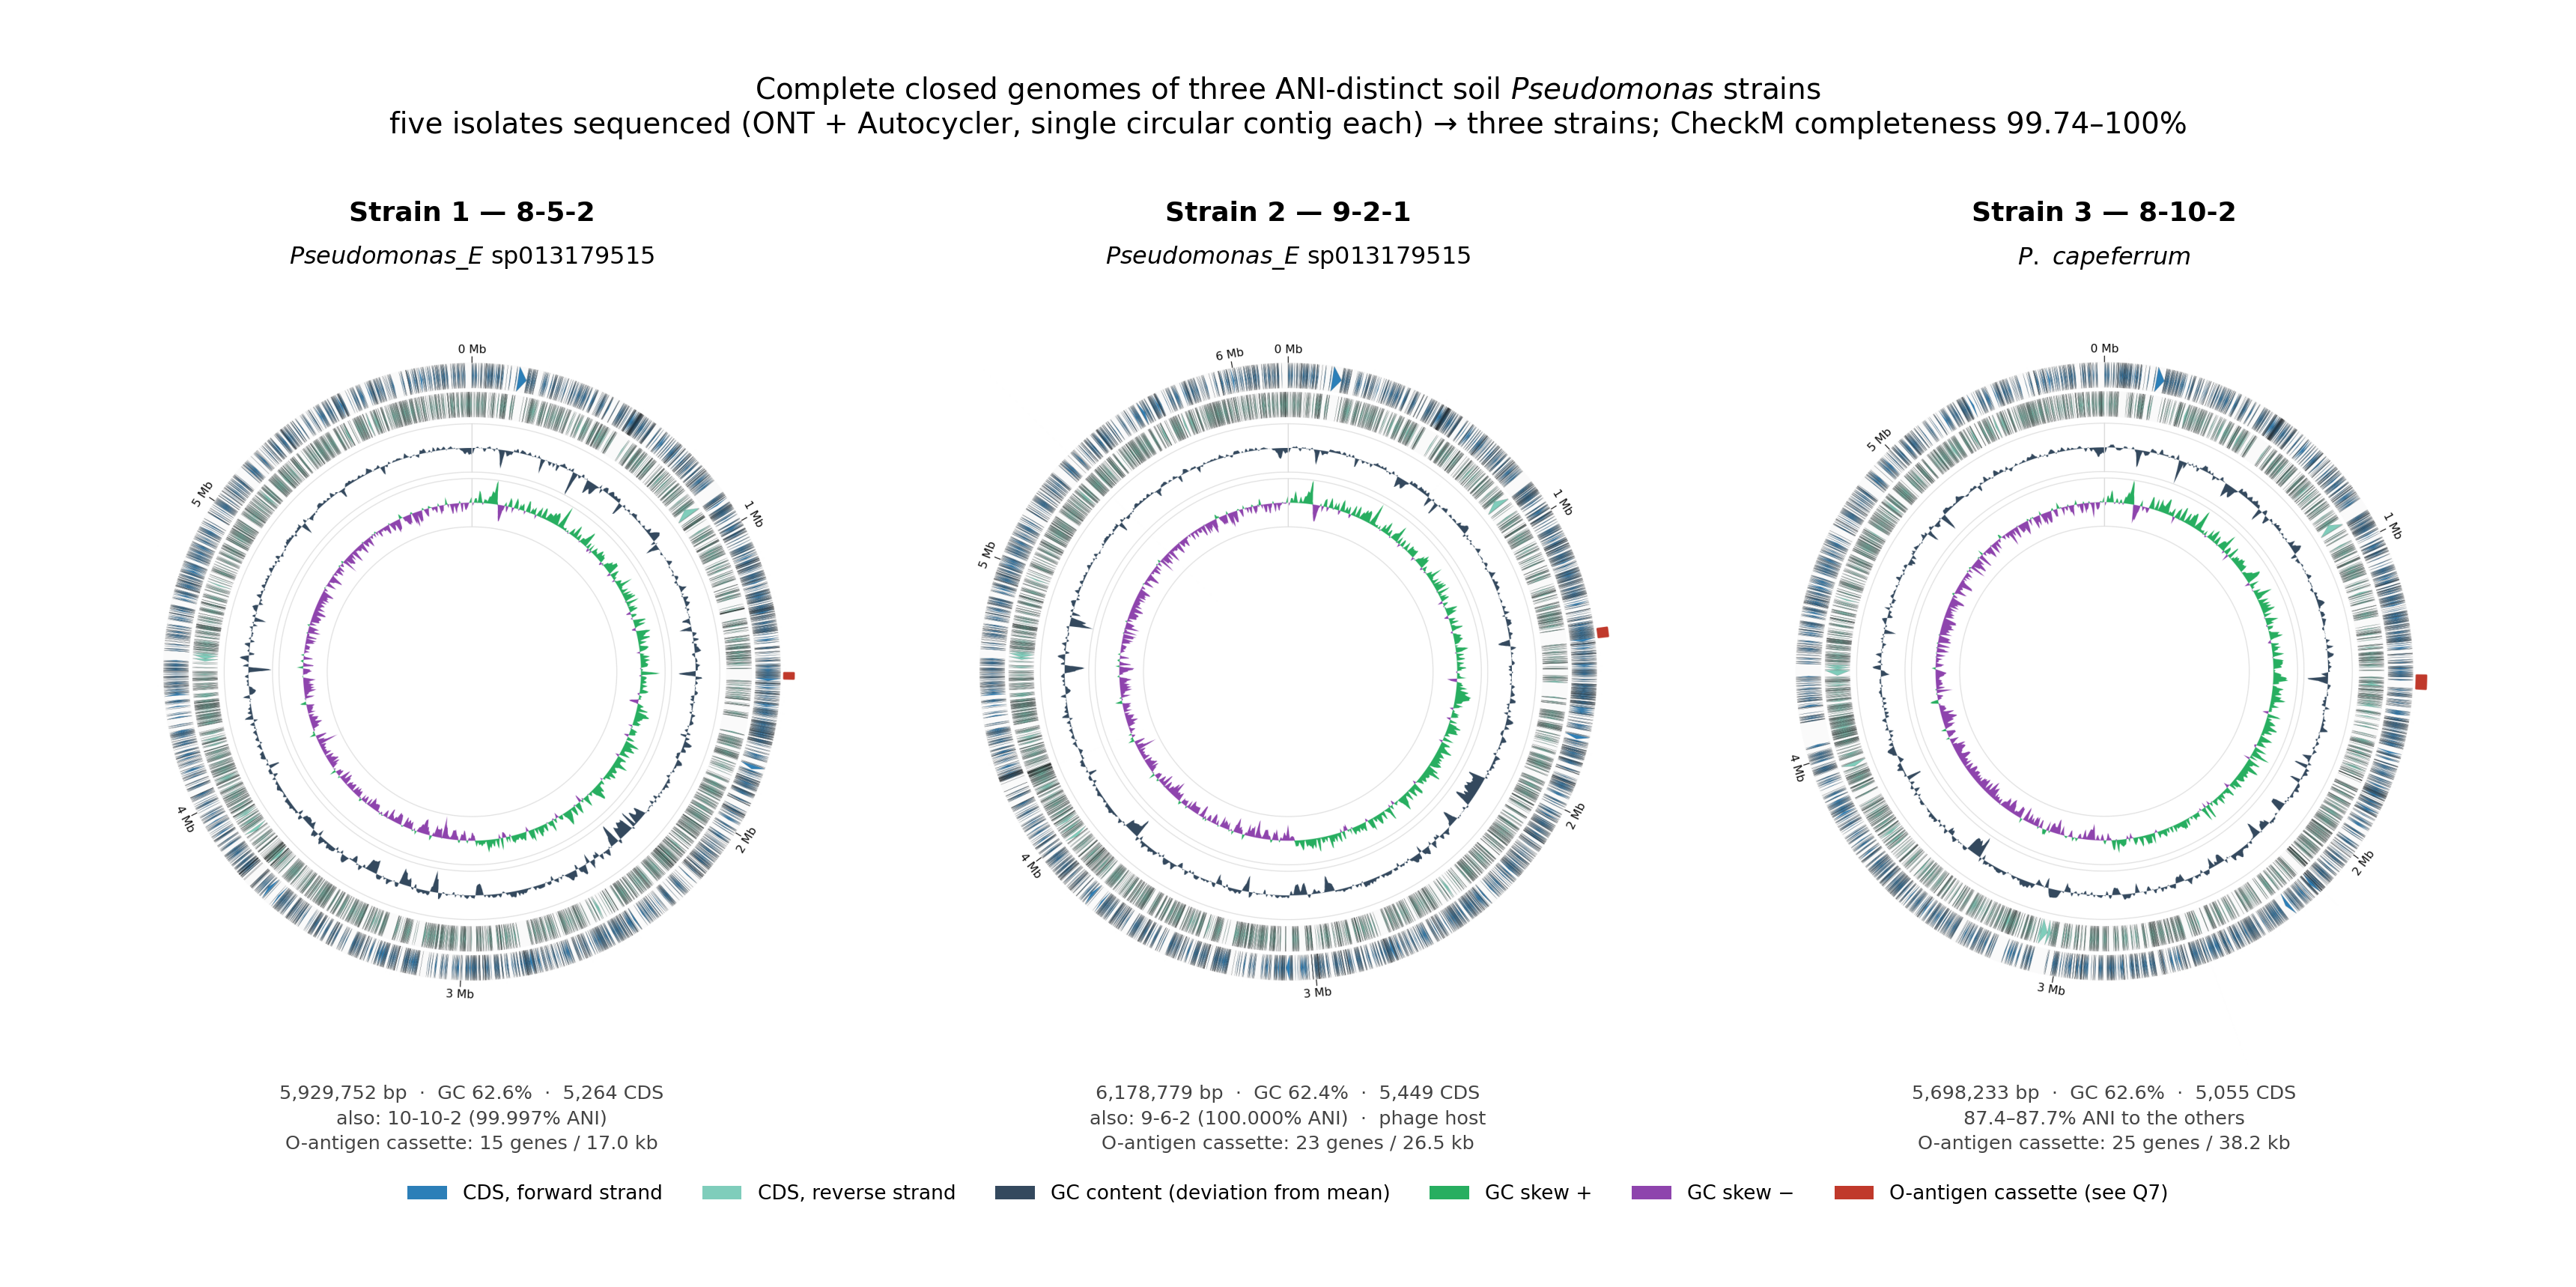
\includegraphics[width=0.95\textwidth,height=0.78\textheight,keepaspectratio]{../../code/output/0729_prof_figures/fig_bacterial_genomes.png}
\end{frame}

\begin{frame}{Backup 6 — phage genome, tail / RBP module}
  \centering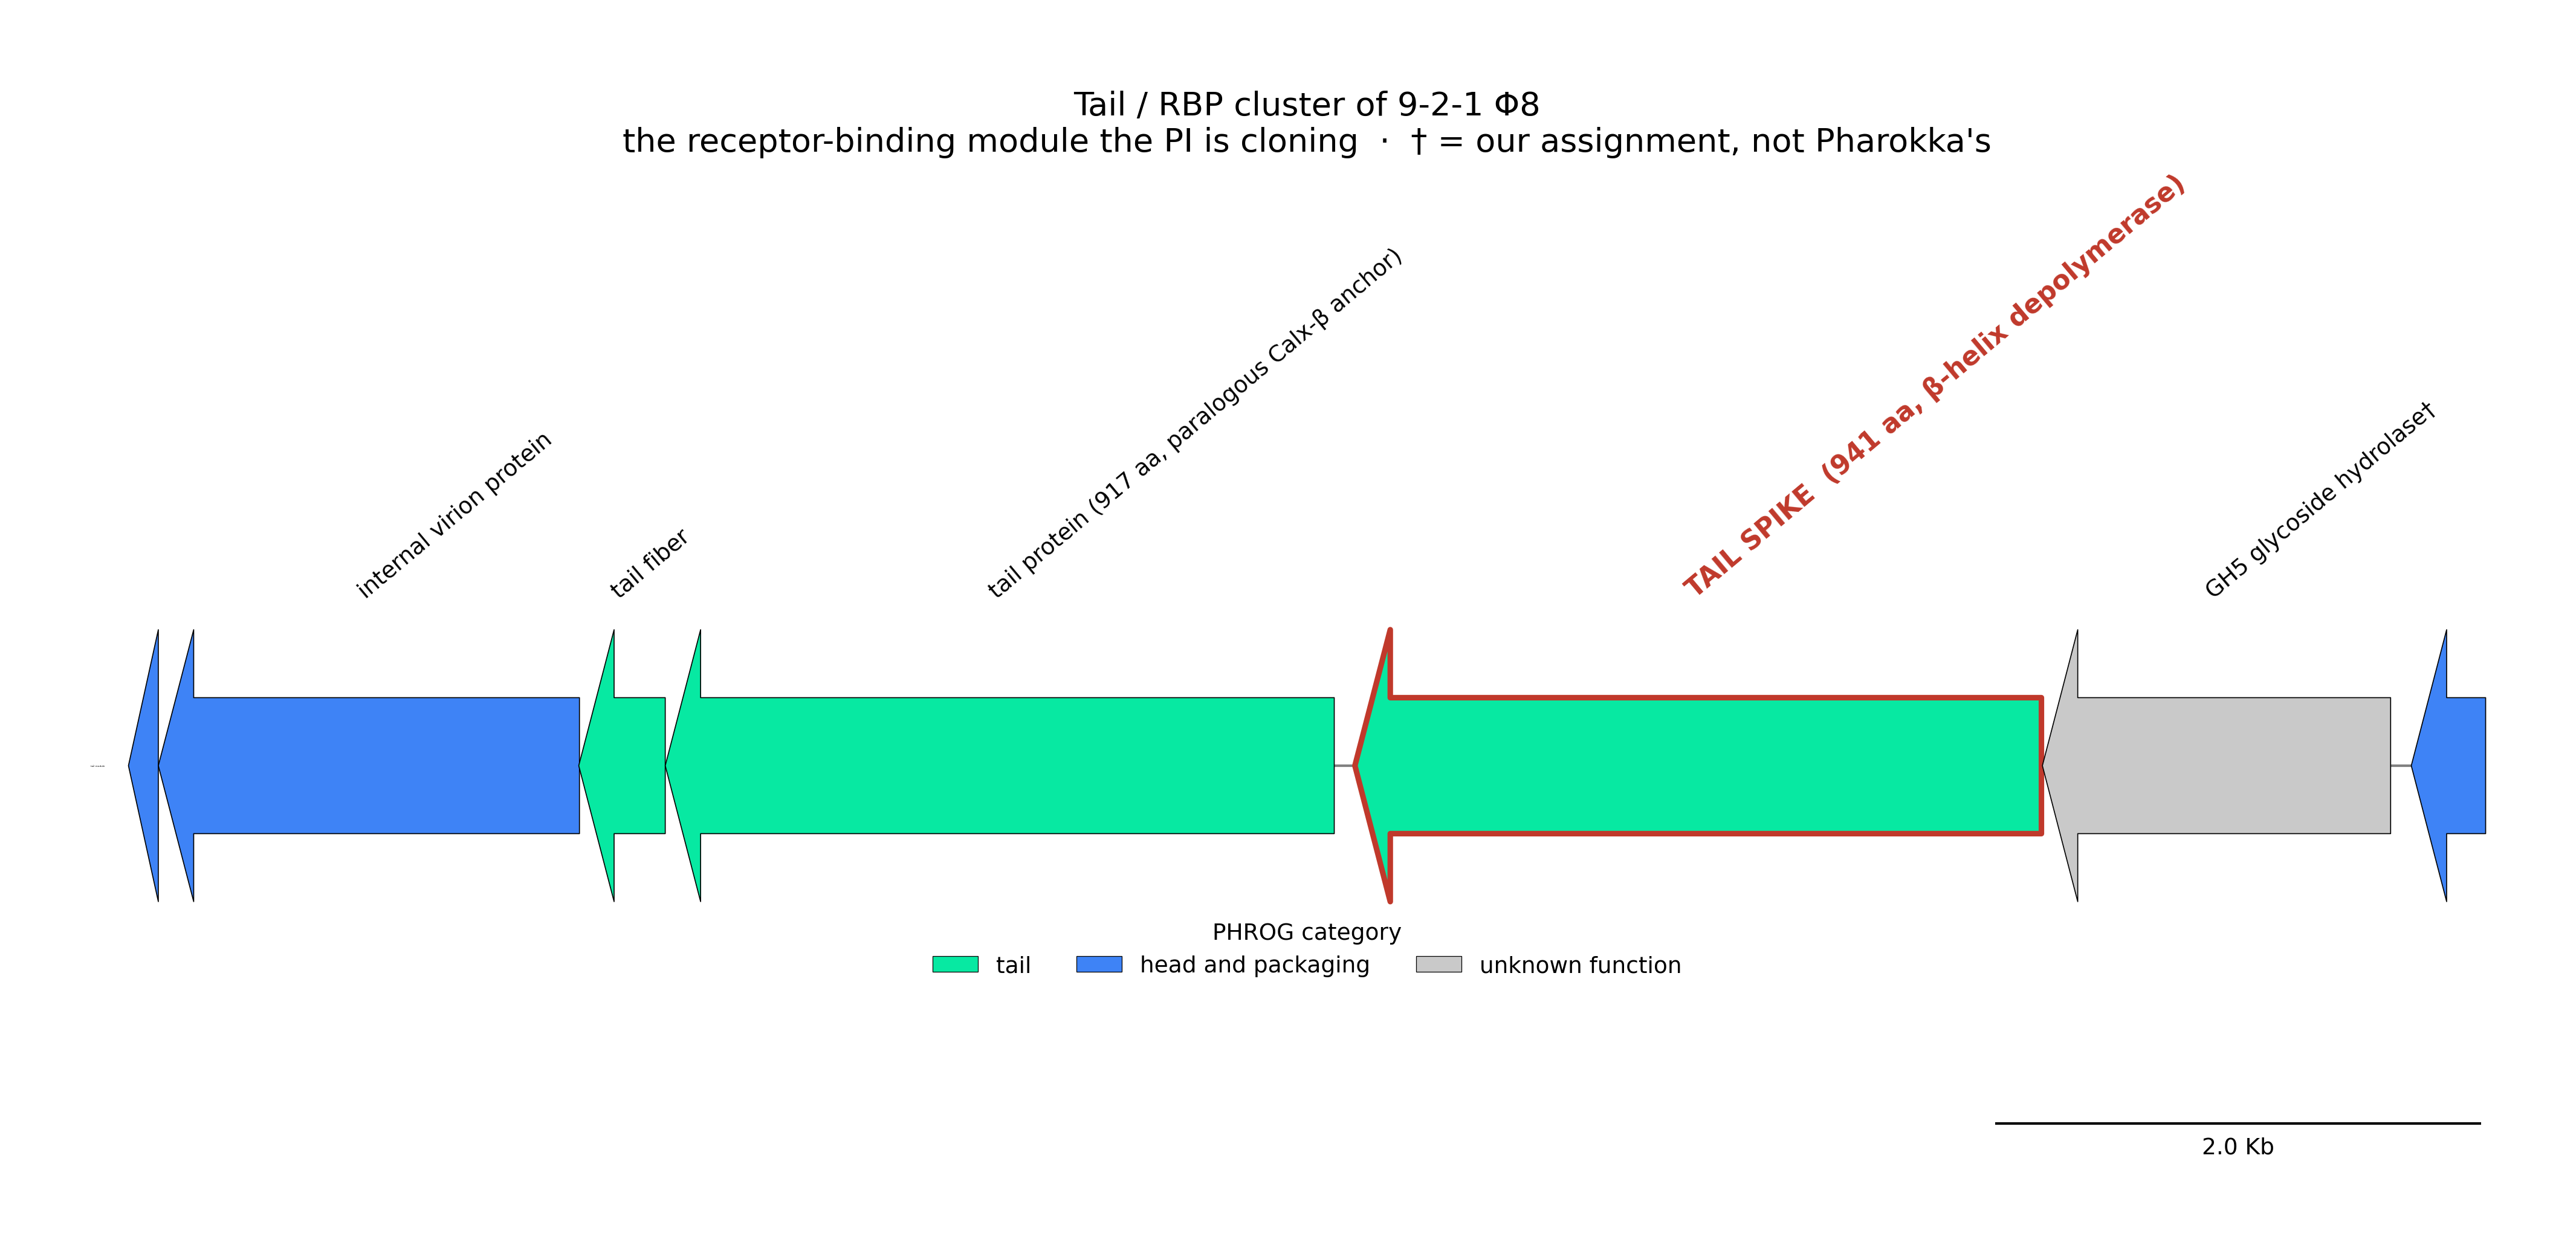
\includegraphics[width=0.98\textwidth,height=0.70\textheight,keepaspectratio]{../../code/output/0729_prof_figures/fig_phage_tail_module.png}\\
  {\scriptsize\color{muted} Numbering is the PI's \texttt{UUAIURNK\_}. The old 0708 genome map is
   mirrored — do not reuse it.}
\end{frame}

\begin{frame}{Backup 7 — enzymatic domains in full (incl.\ CDS\_0012 GH5)}
  \centering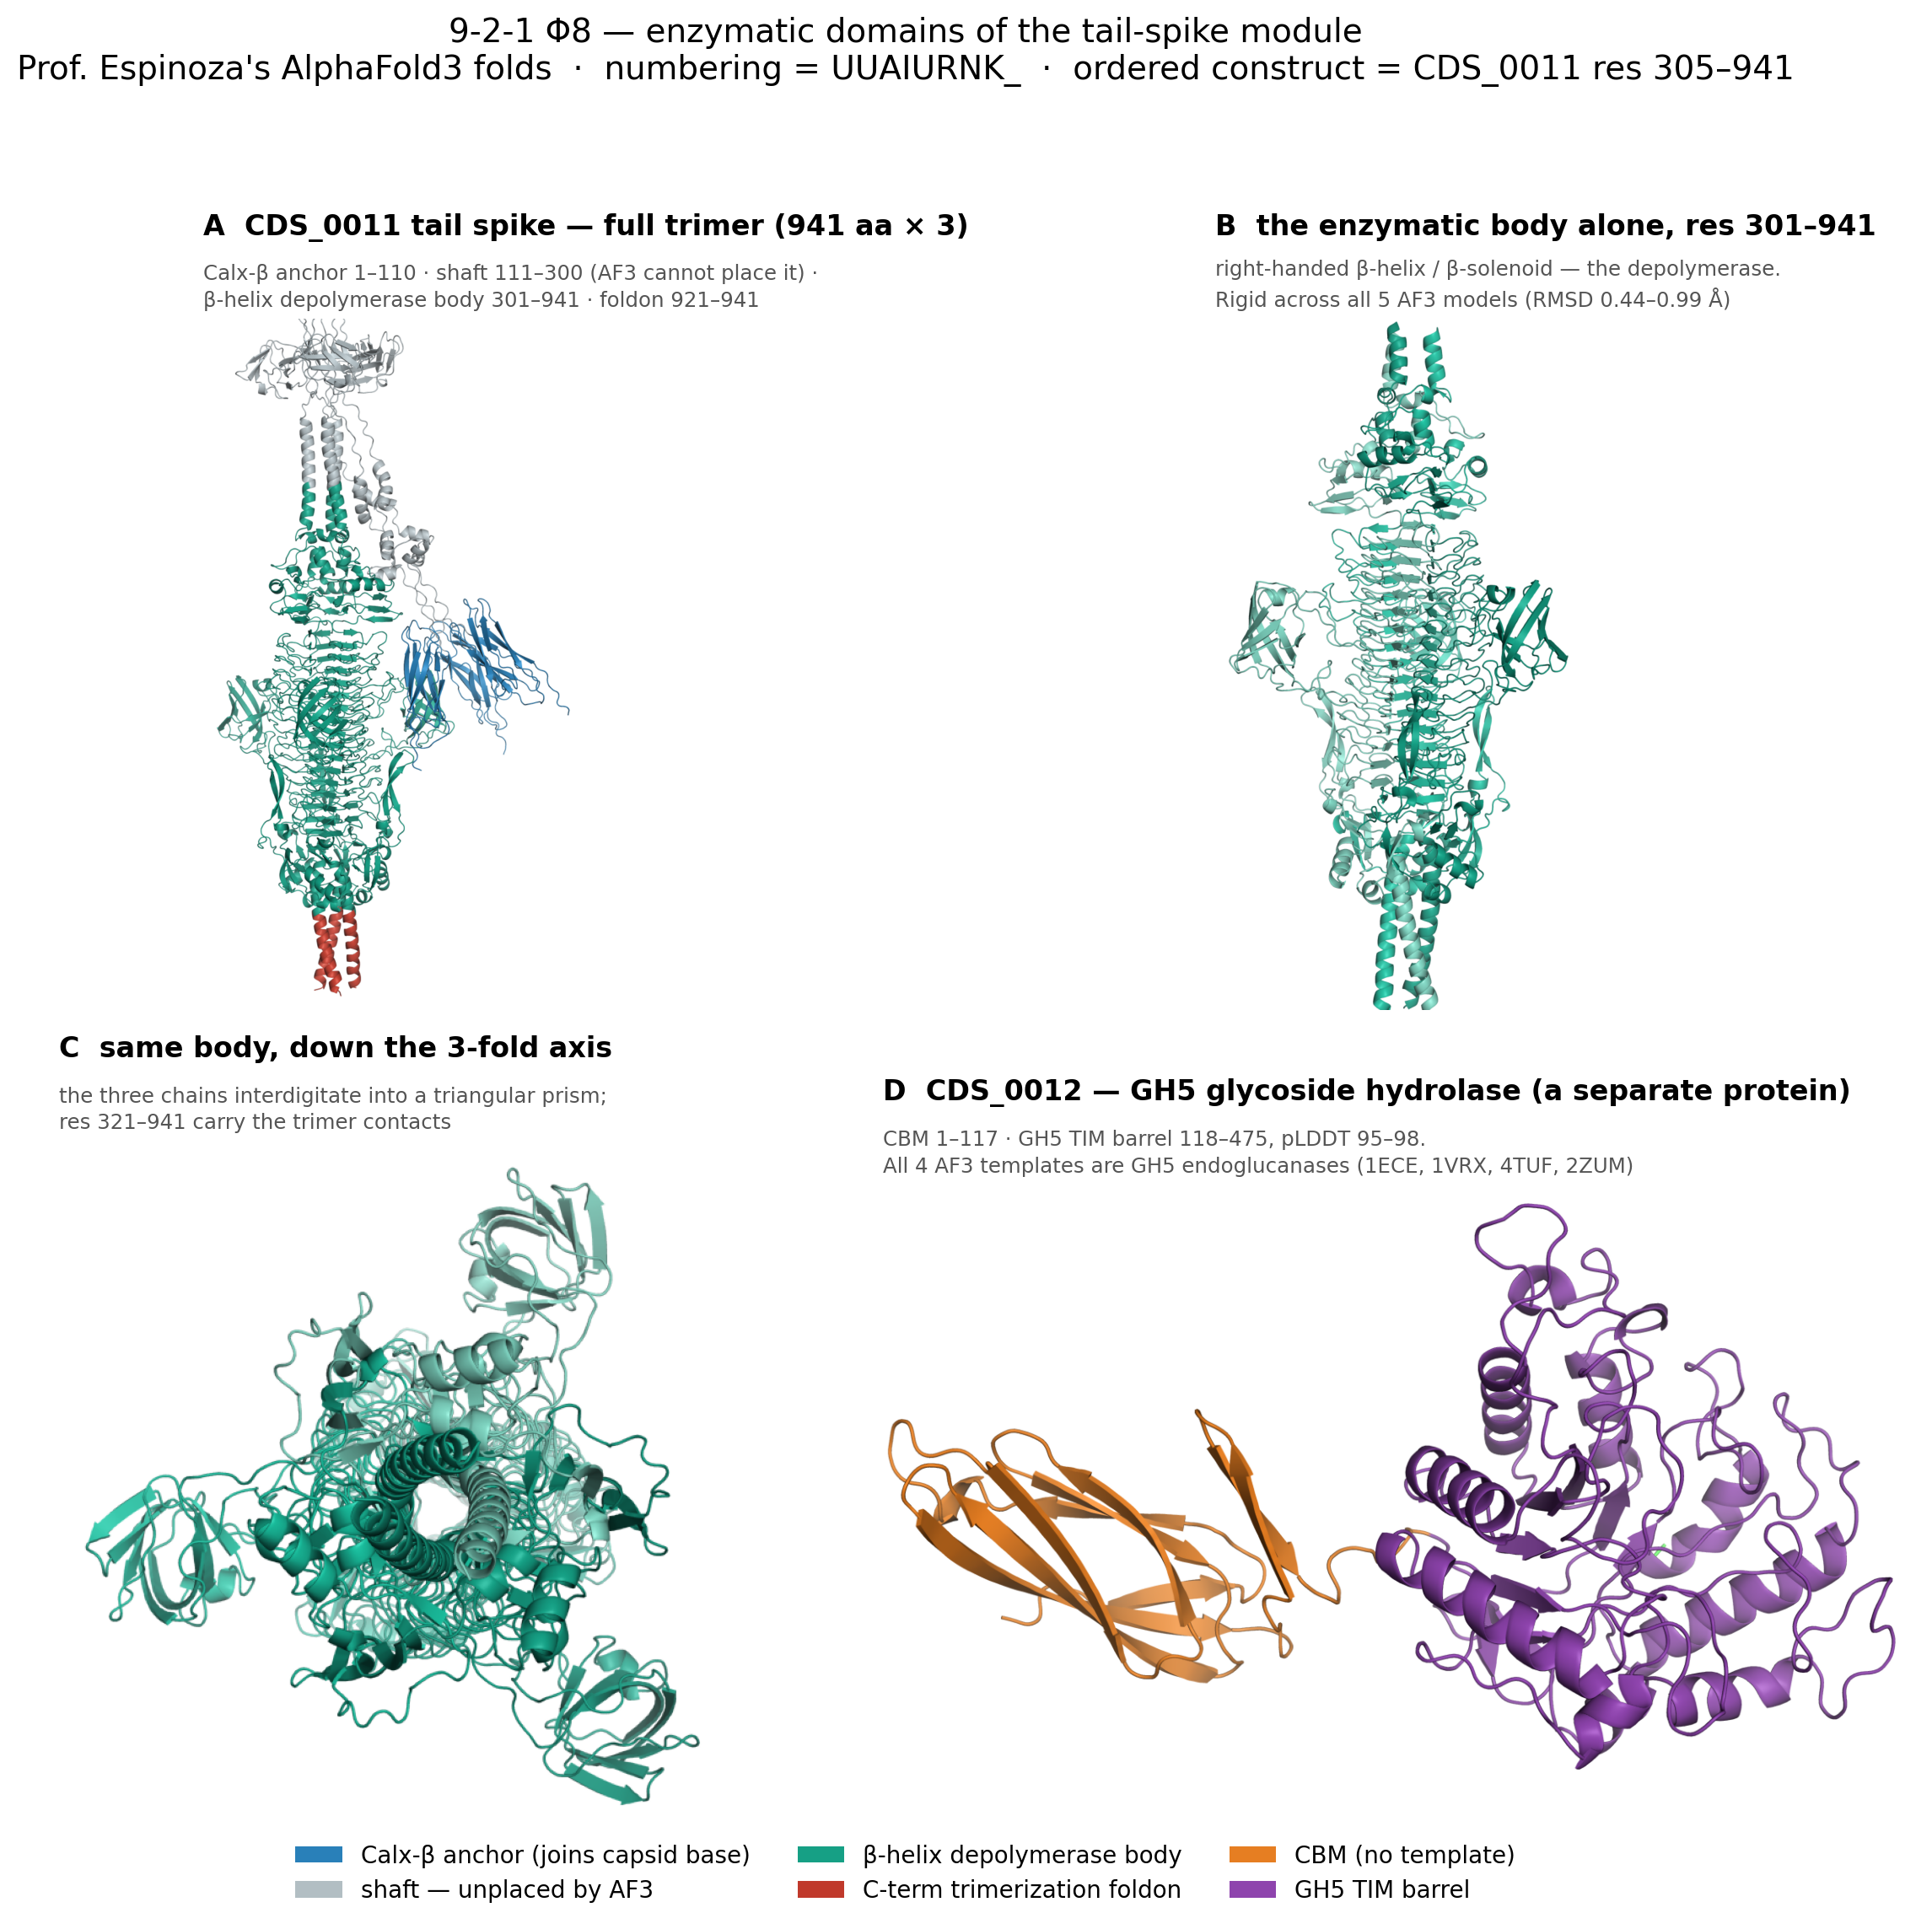
\includegraphics[width=0.68\textwidth,height=0.76\textheight,keepaspectratio]{../../code/output/0729_prof_figures/fig_enzymatic_domains.png}\\
  {\scriptsize\color{muted} Panel D is CDS\_0012 — a \textbf{separate protein}, not a domain of the
   tail spike.}
\end{frame}

\end{document}
